\documentclass[pdftex,12pt,a4paper]{report}
\usepackage{dbstmpl}
\usepackage{subcaption}
\usepackage[utf8]{inputenc}
\usepackage{tikz}
\usepackage{tikzscale}

% Hier die eigenen Daten eintragen
\global\arbeit{Masterarbeit}
\global\titel{Data Science in Zooarchaeology: Analyzing local shape variations in bone findings}
\global\bearbeiter{Stefan Lau}
\global\betreuer{Johannes Niedermayer}
\global\aufgabensteller{PD Dr. Matthias Renz}
\global\abgabetermin{28.08.2015}
\global\ort{München}
\global\fach{Medieninformatik}

\begin{document}

% Deckblatt
\deckblatt

% Erklaerung fuer das Pruefungsamt
\erklaerung

% Zusammenfassung
\begin{abstract}
In this thesis we present a novel algorithm to detect local shape variations between two classes of shapes. Based on local sampling of the shapes, we employ a support vector machine to determine the local separability of the classes. To ensure correctness, we validate the algorithm using synthetically created shapes of bones.

The presented method is then applied to Tali bones from sheep, which are provided as image data. These have been classified by expert knowledge as wild or domestic sheep. We create a semi-automatic extraction pipeline of outlines from the pictures, which feeds the algorithm.

We apply the algorithm to the actual bone data to find the significant variations. The findings are then compared to previous findings from zoo-archaeologists.
\end{abstract}

% Inhaltsverzeichnis
\tableofcontents

% Hier beginnt der eigentliche Text
\chapter{Introduction}

In biology a lot of focus lies on the distinctions between species and within species. These distinctions can be based on the genealogical tree of the animal, its constitution or by other features. While living animals can be examined by several additional means, like their muscular structure or blood levels, this is not as easy for animals that are extinct or deceased for a long time, which are found in zoo-archaeology.

For zoo-archaeologists, archaeological findings of bones are an integral part of their research, since they are one of the sparse remains of the studied animals that are available. From these findings a lot of variables about the animal itself and its environment can be inferred. While a lot of mammals share a similar skeleton, the bones of the animals have varied shapes and sizes depending on multiple variables. These differences in shape and size can be statistically analyzed. The goals of the analysis can be manifold. They can be aimed at emphasizing the distinctions between species, but can also show how the habitat of the animal can influence the frame. While in zoo-archeology only the remains of the animal can be analyzed, biologists use similar methods to analyze the shapes of live animals as well.

These analyses have a long tradition in the field of biology, while the goals are similar to those of data science: Detecting new and interesting information about a data set. But the focus of data scientists in the field of shape are currently different, focusing on shape matching and retrieval. A partnership of the institute for palaeo-anatomy of the Ludwig-Maximilian-University in Munich and the database systems group of the department of computer science allows data scientists to research bone findings to support the zoo-archaeologists.

In this thesis we present a novel algorithm for shape comparison employing data-mining techniques. Our method is based on sampling sections of the shapes outlines in each observation. A support vector machine is used to evaluate the separability of these samples, by extracting features from them and training the SVM. We then employ this algorithm to detect differences in shape between wild and domestic sheep bones that were supplied by the zoo-archaeologists. Furthermore we present a method to classify sheep bones in the field using distances between landmark points and a decision tree classifier. 

In Chapter \ref{chapter:problem-definition} we will describe the problem as it was presented to us by the zoo-archaeologists. Related works to this task are evaluated in Chapter \ref{chapter:related}, highlighting differences between morphometrics and shape matching. Chapter \ref{chapter:basics} will cover the mathematical basics required to comprehend the matter in this thesis. The novel method to find significant shape variations and the preprocessing that is necessary to extract the shapes from the images are introduced in Chapter \ref{chapter:detecting-shape-variations}. Chapter \ref{chapter:measurable-differences} addresses classification of sheep bones using a decision tree based on landmark distances. The experiments that were conducted to validate and apply the presented algorithms are covered in \ref{chapter:experiments}. We discuss the results from these experiments in Chapter \ref{chapter:conclusion} and present possibilities for future research. 

\chapter{Problem Definition}
\label{chapter:problem-definition}

The area of research that this work is located in is the documentation of early domestication of sheep. Previous work by the zoo-archaeologists examined the Talus, a bone located in the ankle joint of mammals. Their goal was to determine differences between domestic and wild sheep that manifest in this bone. This bone was chosen because it is one of the few bones that stayed intact over the time the skeleton rested in the earth. They based their findings on traditional morphometrics as well as geometric morphometrics. Our goal was to confirm and refine the significant variances that the archaeologists found, as well as to automate the process.

\begin{figure}[h]
	\centering
	\begin{subfigure}[b]{0.65\textwidth}
		\centering
		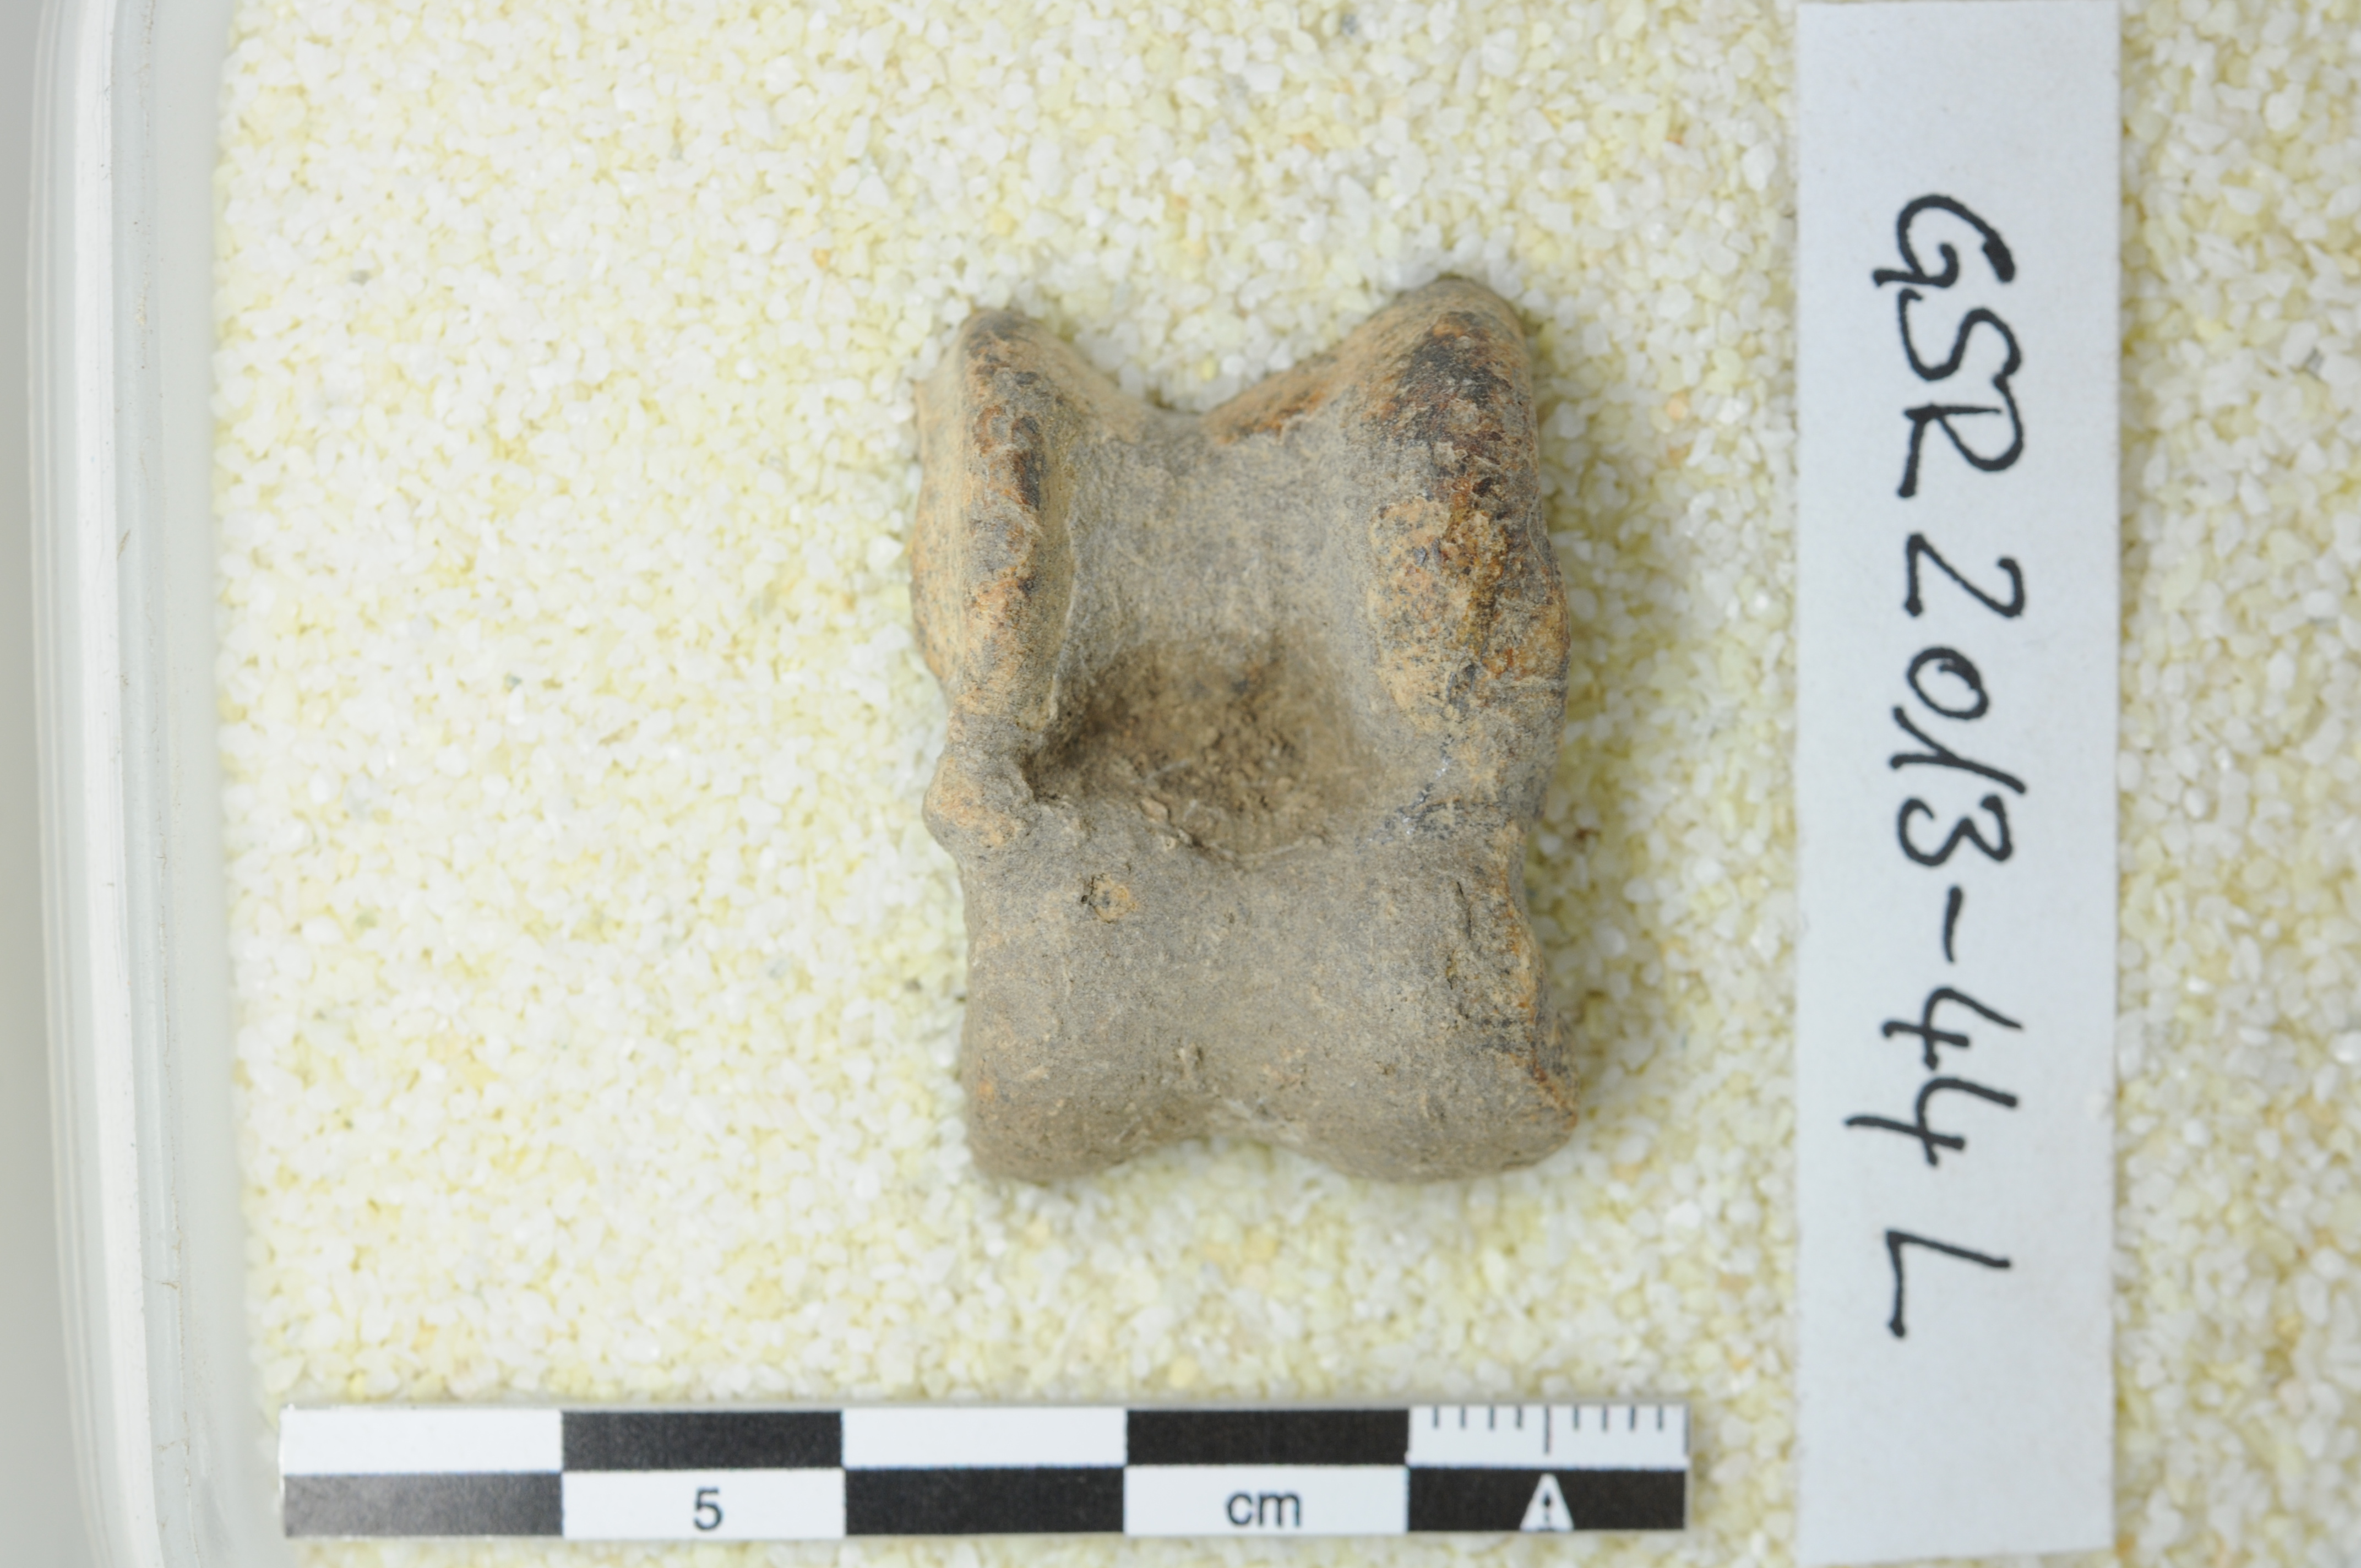
\includegraphics[width=.9\linewidth]{img/example.jpg}
	\end{subfigure}
	\caption{An example for a Talus from a wild sheep}
	\label{fig:problem-example}
\end{figure}


For this purpose we were provided with several images of Tali from four archaeological sites: Manching, Milet, Gusir and Göbekli. All Tali were photographed from approximately the same perspective. An example for one of these images can be seen in Figure \ref{fig:problem-example}. Based on their place of discovery they can be classified through expert knowledge.

Manching bones can be classified as domestic sheep since Manching is located in southern Germany which was not a habitat of wild sheep. The bones from Milet are from the iron age when the wild sheep were extinct in this area and can be classified as domestic sheep as well. Additionally they were found in the temple of Aphrodite, where only domestic sheep were sacrificed, because the sacrifice was required to be done inside the temple and the animal needed to be unharmed. The bones from Gusir and Göbekli are classified as wild sheep, since they originate from a period in which the human species was still organized as hunter-gatherers.

This classification is the basis for this work to locate significant shape variances in the bones. Our goal was to highlight areas one the bone outline where the two classes are separable the most by a classifier, marking it as a characteristic location where the type of sheep can be identified. This would allow the zoo-archaeologists to estimate the class of a bone using a photograph.

Additionally, since relocating a bone finding to another country is difficult, we wanted to provide a method of classification for newly dug out bones, which could be executed using only a caliper rule. This would allow a researcher to identify on-site whether a bone originates from a domestic or a wild sheep. 

\chapter{Related Work}
\label{chapter:related}

The field of shape comparison is divided into two areas. Traditional morphometrics in biology analyze distances, masses, angles and ratios in order to determine differences between species. Shape matching in data science tries to describe shapes with feature vectors to facilitate shape retrieval or shape classification in a database. These two fields exist fairly independent of each other.

\section{Morphometrics in Biology}

Morphometrics were introduced in biology by Blackith et. al in 1971 \cite{blackith1971multivariate}. Their goal was to apply multivariate statistical analysis not only to biology, but to a wide range of fields like geology, sociology and genetics. In the following years, these techniques were applied to determine correlations between certain variables in animals or animal bones and e.g. the habitat or climate. Mainly distances were used for comparison, which causes a problem, because linear distance measurements are often correlated to size \cite{bookstein1985morphometrics}. Geometric morphometrics was introduced to cope with this problem by evaluating coordinates instead of distances, by comparing outlines or landmarks.

Finding correlations in shapes by evaluating their outline usually consisted of using Fourier Analysis to represent the outlines and then using statistical analysis to find correlations. Palmquist et. al. \cite{palmqvist1996comparative} applied this method to findings of human finger bones to differentiate them from bones of several ape species and confirm that they are in fact from the genus Homo. 

In landmark based methods specific points in 2 or 3 dimensions are selected that are used as the input for the method. These points can be located using different methods, like the intersection of structures or as local maxima or minima on the outline. Methods to analyze these coordinates include Procrustes analysis \cite{small1996statistical} or Euclidean distance matrix analysis \cite{lele1991euclidean}.

Modern approaches to geometric morphometrics often analyze the shapes in Kendall shape space, which is a mathematical space introduced by the shape coordinates \cite{mitteroecker2009advances}. Sliding semi-landmarks are often used to fill the space between the landmarks, while maintaining the shape. To visualize differences between shapes, thin plate spline deformation grids are used, which show how the shape of one class is transformed into the other \cite{adams2004geometric}.

\section{Shape Matching in Data Science}

In the context of data science, the focus of research lies in shape matching rather than shape analysis. Shape matching describes the similarity between two shapes by a distance. This can be used e.g. to fetch similar shapes from a database or classify shapes into several groups.

Veltkamp et. al. present a survey of shape matching algorithms in \cite{veltkamp2001shape}. Distance measures used include Minkowski Distance, Bottleneck Distance or the Turning Function Distance. All of these measures do not employ key points that are selected on the outline of the shape. Other methods like the shape context by Belongie et. al. \cite{belongie2002shape} employ correspondence matching, but generalize the results to the full shape as well.

The book \grqq Shape analysis and classification\grqq  by da Fontoura Costa et al. \cite{da2010shape} covers shape classification, but does not mention classification based on local differences, which we want to employ in this thesis.

An approach to classification by local key points has been done by Mhamdi et. al . \cite{mhamdi2014local}. They represent the critical points by a set of size functions and use the resulting similarity measure for classification.

\chapter{Mathematical Basics}
\label{chapter:basics}

\section{Splines}
\label{section:splines}

\begin{figure}[h]
	\centering
	\begin{subfigure}[b]{0.3\textwidth}
		\centering
		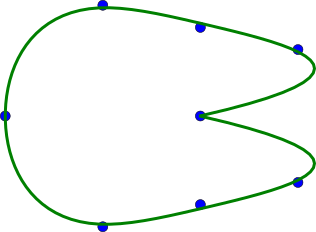
\includegraphics[width=.9\linewidth]{img/basics/splines.pdf}
	\end{subfigure}
	\caption{Interpolated smooth spline}
	\label{fig:basics-splines}
\end{figure}

A spline is a parameterized representation of a function that consists of several pieces of polynomial functions. The end points of these pieces are connected while ensuring smoothness in between them. Splines can be used to represent arbitrary curves in computer graphics. For our purposes we used non-uniform cubic B-Splines to represent the bone outlines. A B-Spline of degree $p$ is described by points $\vec{p}_0 \cdots p_{n-p}$ called knots and a knot vector $t = (t_1, \cdots t_{n})$, which describes the weight of those knots.  B-Splines have a defined set of base functions in which they describe their pathway and can be calculated recursively.

\begin{equation}
\begin{split}
& B_i^0(t) = \left\{
\begin{matrix} 
1 & \mathrm{if} \quad t_i \leq t < t_{i+1} \\
0 & \mathrm{otherwise} 
\end{matrix} \right. \\
& B_i^p(t) = \frac{t - t_i}{t_{i+p} - t_i} B_i^{p-1}(t) + \frac{t_{i+p+1} - t}{t_{i+p+1} - t_{t+1}} B_{i+1}^{p-1}(t)
\end{split} 
\end{equation}

The B-Spline curve is then defined as:

\begin{equation}
\vec{s}(t) =  \sum_{i=1}^{n-p} \vec{p}_i B_i^p(t)
\end{equation}

The interpolation of spline curves is preferred over polynomial interpolation, because it avoids Runge's phenomenon, which manifests in high frequency oscillations between control points. In this thesis we use the spline interpolation algorithm from scikit-learn \cite{pedregosa2011scikit}. This algorithm also allows for smoothing of the spline, which we apply to a small degree to reduce the edges on our bone outlines. Figure \ref{fig:basics-splines} shows a smoothed spline interpolated from several points.

\section{Principal Component Analysis}
\label{section:pca}

Principal Component analysis is a statistical technique to decrease dimensionality of a data set, while converting the values into linearly uncorrelated variables that are called principal components. These components are sorted by variance so latter components can be omitted from observations without changing the expressiveness of the data.

Principal component analysis works on the derivations from the mean data in $DB$.

\begin{equation}
\begin{split}
& \vec{\mu} = \frac{1}{|DB|} \sum_{\vec{o} \in DB}  \vec{o} \\
& DB_\mu = \{ \vec{o} - \vec{\mu} \mid \vec{o} \in DB \}
\end{split}
\end{equation}

The principal components can be obtained by calculating the eigenvectors of the covariance matrix defined by the observations after subtracting the mean values. These vectors are by definition orthogonal to each other leading to uncorrelated variables. The covariance matrix can  be created from a matrix $\mathbf{D}$ with all objects from $DB_\mu$ as rows.

\begin{equation}
\mathbf{C} = \frac{1}{|DB|-1} \mathbf{D}^* \cdot \mathbf{D}
\end{equation}

The extraction of eigenvectors is usually done by an numeric algorithm, in our case the implementation from scikit-learn \cite{pedregosa2011scikit}. The objects in the database can now be represented by using the eigenvectors as a new basis. The eigenvectors can then be sorted by their variances in data and limited to the number of dimensions necessary for the task.

\section{Cluster Analysis}

Cluster analysis is an integral part of data mining. The goal of cluster analysis is to group objects that are similar to each other. The objects are represented as n-dimensional vectors while the similarity of objects translates into a low distance between the vectors. The objects are also often referred to as observations. In this thesis we will use two types of clusterings, which we present in this section.

\begin{figure}[h]
	\centering
	\begin{subfigure}[b]{0.45\textwidth}
		\centering
		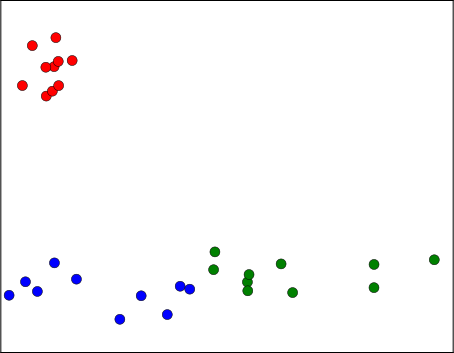
\includegraphics[width=.9\linewidth]{img/basics/kmeans.pdf}
		\subcaption{K-means}
		\label{fig:basics-clustering-k-means}
	\end{subfigure}
	\begin{subfigure}[b]{0.45\textwidth}
		\centering
		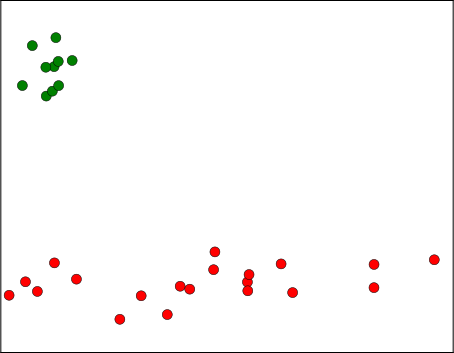
\includegraphics[width=.9\linewidth]{img/basics/dbscan.pdf}
		\subcaption{DBSCAN}
		\label{fig:basics-clustering-dbscan}
	\end{subfigure}
	\caption{Clustering algorithms}
	\label{fig:basics-clustering}
\end{figure}

\subsection{K-Means}

K-means clustering is a partitioning clustering algorithm, a kind of algorithm that separates space into segments, with all points in one segment belonging to a cluster. In k-means clustering, each cluster $C_i$ is represented by its centroid $\mu_i$. An object belongs to the cluster with the closest centroid. The partitioning manifests in a Voronoi cells built from the representatives from each cluster. The number of clusters $k$ is a parameter that needs to be specified to fit the data.

\begin{equation}
\vec{\mu}_i = \frac{1}{|C_i|} \sum_{\vec{o} \in C_i}\vec{o}
\end{equation}

The algorithm to create the clustering is iterative. The simplest way is to initially select random points as centroids for each cluster. Then the cluster memberships are reevaluated and the centroids are recalculated. These two steps are iterated until a maximum number of iterations is reached or the following compactness criterion is met:

\begin{equation}
\sum\limits_{C_i \in CL} \sum\limits_{\vec{o} \in C_i} dist(\vec{o}, \vec{\mu}_i)^2 <= \xi
\end{equation}

Other initialization methods exist as well, and the algorithm varies slightly between implementations, e.g. reevaluating cluster memberships and centroids after each membership assignment. 

The clusters created by k-means clustering are spherical compact clusters as visible in Figure \ref{fig:basics-clustering-k-means}. This is caused by the distance being used as a distance measure and as a measure for cluster scatter.

\subsection{DBSCAN}

The goal of the DBSCAN cluster algorithm is to group objects into areas of high densities, separated by areas of low densities. The objects in the low density areas are marked as noise while all objects inside each high density area are belonging to a single cluster. DBSCAN works with a concept of densibility reachability, based on parameters $minPts$ and $\epsilon$:

\begin{itemize}
	\item
	Core points: Each point that satisfies: \\$|RQ(\vec{p}, \epsilon) = \{  \vec{o} \in DB \mid dist(\vec{o},\vec{p}) <= \epsilon  \}| \geq minPts$
	
	 \item
	 $\vec{q}$ is direct-density-reachable from $\vec{p}$: $\vec{q} \in RQ(\vec{p}, \epsilon)$ and $\vec{p}$ is core point
	 
	 \item
	 $\vec{q}$ is density-reachable from $\vec{p}$: There exists a chain of direct-density-reachable objects between $\vec{q}$ and $\vec{p}$
	 
	 \item
	 $\vec{q}$ and $\vec{p}$ are density-connected: $\vec{p}$ and $\vec{q}$ are both density-reachable from an object
\end{itemize}

Clusters are created from sets of density-connected points. These points are found by expanding clusters with range queries, trying to find direct-density-reachable points or core points until each object has either been classified as belonging to a cluster or noise.

Figure \ref{fig:basics-clustering-dbscan} shows a clustering created with DBSCAN. The clusters generated with DBSCAN can be of arbitrary shape as long as they have a similar density. A change in density is necessary for the algorithm to separate clusters. 

\section{Support Vector Machines}

A support vector machine is a classifier that separates a set of objects into two classes. As a supervised method it needs to be trained using training data and then can be applied to new objects to classify them. The methodology is to create a hyperplane in the feature space which separates the two classes from each other. The plane is created to have a maximum distance from the nearest data point of each class, facilitating good generalization. These data points are called support vectors and the distance to the hyperplane is known as the margin.

\begin{figure}[h]
	\centering
	\begin{subfigure}[b]{0.75\textwidth}
		\centering
		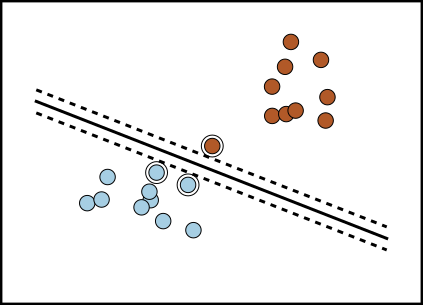
\includegraphics[width=.9\linewidth]{img/basics/svm.pdf}
	\end{subfigure}
	\caption{Support Vector Machine}
	\label{fig:basics-svm}
\end{figure}

Figure \ref{fig:basics-svm} shows a support vector machine. The support vectors are highlighted as the double-outlined points. The separating hyperplane is the solid line while the margin is the distance between the dotted lines.

To train the support vector machine an optimization problem needs to be solved. For a set of observations $\vec{x_i}$ and their classes $c_i \in \{ -1, 1 \}$, the two dotted planes can be described as:

\begin{equation}
\begin{split}
	& \vec{w} \cdot \vec{x} - b = 1 \\
	& \vec{w} \cdot \vec{x} - b = -1
\end{split}
\end{equation}

The distance between these planes is $\frac{2}{||w||}$, so $||w||$ needs to be minimized to maximize the margin. Usually this is transformed into a quadratic optimization problem shown in Equation \ref{eq:svm}, which is subject to the second term shown in Equation \ref{eq:svm}. This problem can be solved efficiently.

\begin{equation}
\label{eq:svm}
\begin{split}
& \arg\min_{\vec{w}, b} \frac{1}{2} ||\vec{w}||^2 \\
& c_i (\vec{w} \vec{x_i} - b) >= 1
\end{split}
\end{equation}

Since it is not always possible to separate the two classes linearly, it is necessary to introduce an error term into the optimization. This process is called soft margin optimization, and will create a hyperplane that splits the examples as cleanly as possible. For this purpose positive error terms $\xi_i$ are introduced that represent the degree of misclassification of $\vec{x}_i$. The optimization problem is then adapted to use these error terms:

\begin{equation}
\arg\min_{\vec{w}, b} \left(\frac{1}{2} ||\vec{w}||^2 + C \sum_{i=1}^{n} \xi_i \right)
\end{equation}

When classifying with the support vector machine, it needs to be determined on which side of the separating hyperplane the observation is located. This can be determined by evaluating the direction of the vector to the observation $\vec{o}$:

\begin{equation}
c_i = sign(\vec{w} \vec{o} - b)
\end{equation}

For our work we are using the LinearSVC implementation from scikit-learn \cite{pedregosa2011scikit}.

\section{Decision Trees}
\label{sec:basics-decision-trees}

The decision tree is one of the few classifiers which provides the user with explicit knowledge about the decision process. Similarly to the SVM, it is from the class of supervised classification mechanisms, requiring training data. A decision tree is a tree with the following properties:

\begin{itemize}
	\item An inner node represents an attribute
	\item A leaf node represents one of the classes
	\item An edge represents a test based on the attribute of the parent node
\end{itemize}

In most decision trees an inner node always has two children, so only binary splits are performed. Exactly one of the test needs to pass to perform the split.

\begin{figure}[h]
	\centering
	\begin{subfigure}[b]{0.65\textwidth}
		\centering
		
\resizebox{\textwidth}{!}{
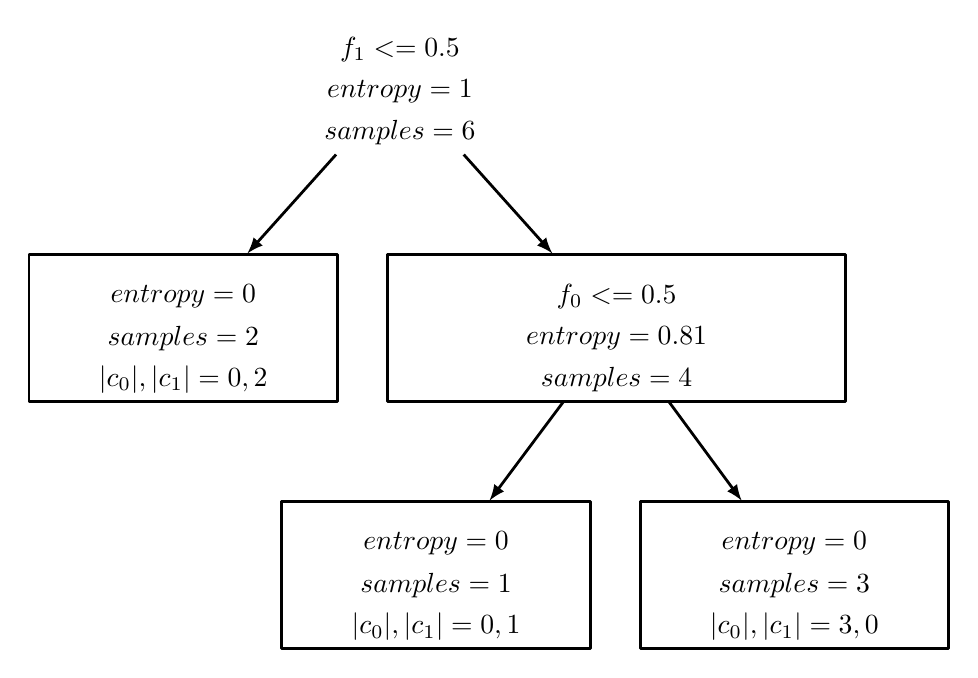
\begin{tikzpicture}[>=latex,line join=bevel,]
  \pgfsetlinewidth{1bp}
  %%
  \pgfsetcolor{black}
  % Edge: 0 -> 1
  \draw [->] (110.52bp,177.87bp) .. controls (102.66bp,169.1bp) and (93.739bp,159.15bp)  .. (78.586bp,142.25bp);
  % Edge: 0 -> 2
  \draw [->] (156.48bp,177.87bp) .. controls (164.34bp,169.1bp) and (173.26bp,159.15bp)  .. (188.41bp,142.25bp);
  % Edge: 2 -> 3
  \draw [->] (192.35bp,88.868bp) .. controls (185.93bp,80.272bp) and (178.66bp,70.549bp)  .. (165.74bp,53.25bp);
  % Edge: 2 -> 4
  \draw [->] (230.36bp,88.868bp) .. controls (236.68bp,80.272bp) and (243.83bp,70.549bp)  .. (256.56bp,53.25bp);
  % Node: 1
  \begin{scope}
  	\definecolor{strokecol}{rgb}{0.0,0.0,0.0};
  	\pgfsetstrokecolor{strokecol}
  	\draw (111.0bp,142.0bp) -- (0.0bp,142.0bp) -- (0.0bp,89.0bp) -- (111.0bp,89.0bp) -- cycle;
  	\draw (55.5bp,126.8bp) node {$entropy = 0$};
  	\draw (55.5bp,111.8bp) node {$samples = 2$};
  	\draw (55.5bp,96.8bp) node {$|c_0|, |c_1| = 0,  2$};
  \end{scope}
  % Node: 0
  \begin{scope}
  	\definecolor{strokecol}{rgb}{0.0,0.0,0.0};
  	\pgfsetstrokecolor{strokecol}
  	\draw (133.5bp,215.8bp) node {$f_1 <= 0.5$};
  	\draw (133.5bp,200.8bp) node {$entropy = 1$};
  	\draw (133.5bp,185.8bp) node {$samples = 6$};
  \end{scope}
  % Node: 3
  \begin{scope}
  	\definecolor{strokecol}{rgb}{0.0,0.0,0.0};
  	\pgfsetstrokecolor{strokecol}
  	\draw (202.0bp,53.0bp) -- (91.0bp,53.0bp) -- (91.0bp,0.0bp) -- (202.0bp,0.0bp) -- cycle;
  	\draw (146.5bp,37.8bp) node {$entropy = 0$};
  	\draw (146.5bp,22.8bp) node {$samples = 1$};
  	\draw (146.5bp,7.8bp) node {$|c_0|, |c_1| = 0,  1$};
  \end{scope}
  % Node: 2
  \begin{scope}
  	\definecolor{strokecol}{rgb}{0.0,0.0,0.0};
  	\pgfsetstrokecolor{strokecol}
  	\draw (294.0bp,142.0bp) -- (129.0bp,142.0bp) -- (129.0bp,89.0bp) -- (294.0bp,89.0bp) -- cycle;
  	\draw (211.5bp,126.8bp) node {$f_0 <= 0.5$};
  	\draw (211.5bp,111.8bp) node {$entropy = 0.81$};
  	\draw (211.5bp,96.8bp) node {$samples = 4$};
  \end{scope}
  % Node: 4
  \begin{scope}
  	\definecolor{strokecol}{rgb}{0.0,0.0,0.0};
  	\pgfsetstrokecolor{strokecol}
  	\draw (331.0bp,53.0bp) -- (220.0bp,53.0bp) -- (220.0bp,0.0bp) -- (331.0bp,0.0bp) -- cycle;
  	\draw (275.5bp,37.8bp) node {$entropy = 0$};
  	\draw (275.5bp,22.8bp) node {$samples = 3$};
  	\draw (275.5bp,7.8bp) node {$|c_0|, |c_1| = 3,  0$};
  \end{scope}
  %
\end{tikzpicture}
}

	\end{subfigure}
	\caption{Decision tree based on data in Appendix \ref{appendix:table:decision-tree}}
	\label{fig:basics-decision-tree}
\end{figure}

The tree is built using training data by iteratively selecting the next attribute for a split for each of the current leaf nodes until only observations of one class are contained in all leaf nodes. The split strategy defines the next attribute that is selected for a split. The most well known split strategies are by maximum information gain or by Gini index.

The maximum information gain split strategy is based on entropy. Entropy is an amount of uncertainty and is high if the dataset is random and low when its less random. The information gain of an attribute that partitions a set $T$ of classes $c_i$ with relative frequencies $p_i$ into multiple sets $T_1, ..., T_n$ is defined as:

\begin{equation}
\begin{split}
	& entropy(T) = - \sum_{i=1}^{k} p_i \log_2 p_i \\	
	& gain(T,A) = entropy(T) - \sum_{i=1}^{m} \frac{|T_i|}{T} entropy(T_i)
\end{split}
\end{equation}

The Gini index is a statistical measure to represent uneven distributions. For a maximum uneven distribution of all observations the Gini index will be one and for a even distribution it will be $0.5$. A split is done in the attribute with the maximum Gini index.

\begin{equation}
\begin{split}
& gini(T) = 1 - \sum_{i=1}^{k} p_i^2 \\
& ginisplit(T,A) = \sum_{i=1}^{m} \frac{|T_i|}{T} gini(T_i) 
\end{split}
\end{equation}

After training the decision tree all training data is classified correctly. Pruning might be applied afterwards to reduce overfitting and thus make the classifier more generalizable. It might also be applied to satisfy external conditions like a maximum tree depth or a minimum support for each leaf node. Depending on the goal multiple pruning strategies exist, which we will not further extend on in this thesis.

To classify using a decision tree we start at the root of the tree and follow the path that our attribute values define. When we reach a leaf node, the majority class of the leaf node is the class we use for the observation. For small decision trees this can be done manually. Figure \ref{fig:basics-decision-tree} shows a decision tree build using information gain and the associated data. A new observation can be classified manually using two comparisons.

In this thesis we are using the decision tree implementation from scikit-learn \cite{pedregosa2011scikit}.

\chapter{Detection of Local Shape Variations}
\label{chapter:detecting-shape-variations}

\section{Overview}

\begin{figure}[h]
	\centering
	\begin{subfigure}[b]{0.95\textwidth}
		\centering
		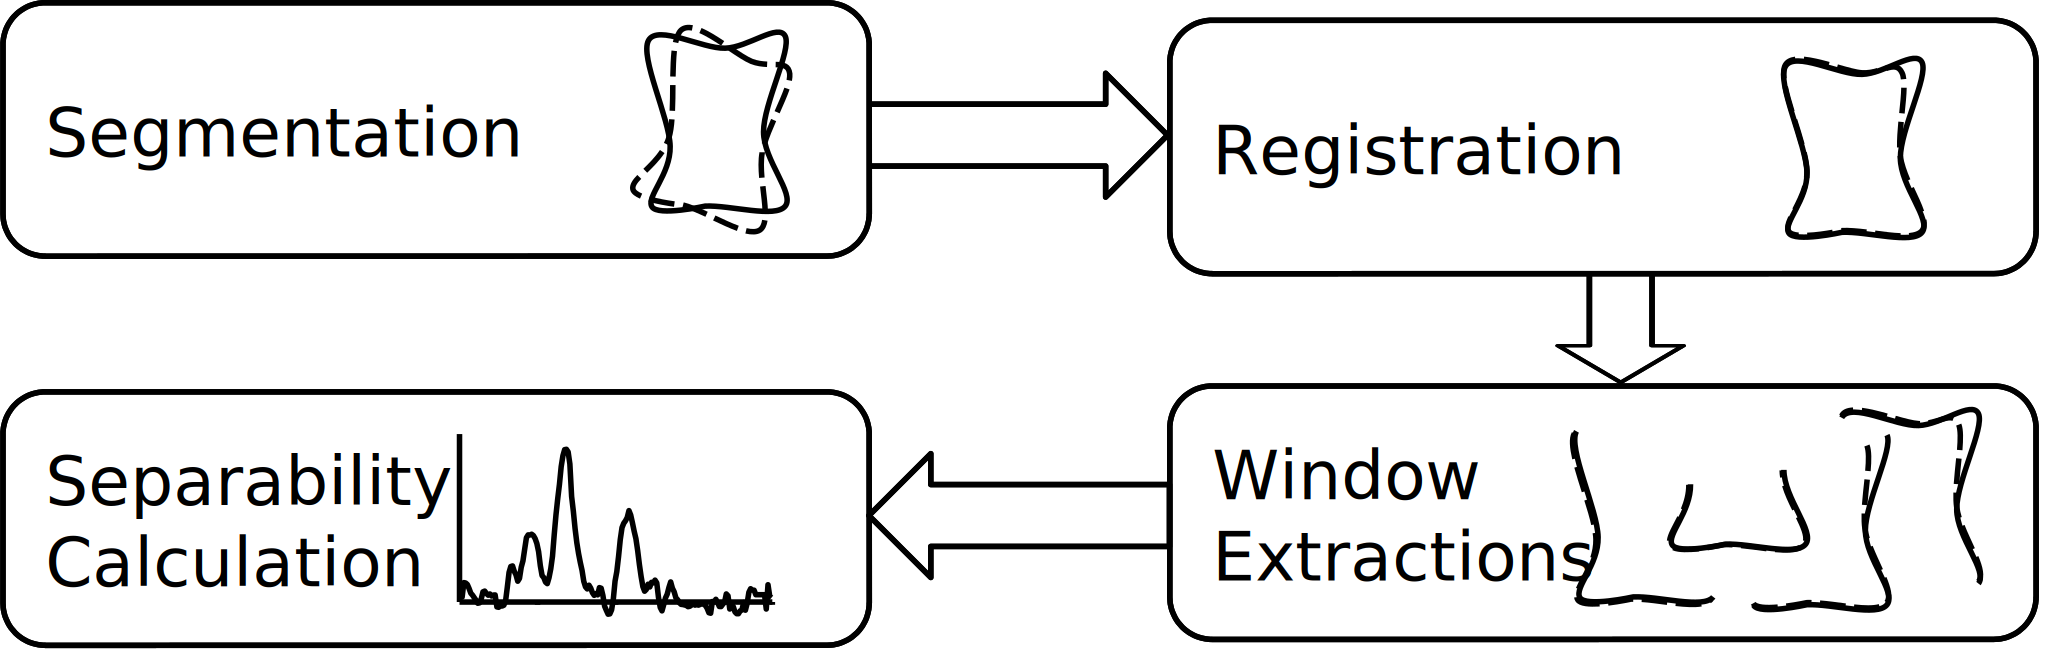
\includegraphics[width=1\linewidth]{img/process.pdf}
	\end{subfigure}
	\caption{Process for finding shape differences}
	\label{fig:process}
\end{figure}

Several steps are necessary to facilitate detecting local shape variations using the data we were provided with. The starting point was a series of images from the Talus of sheep, which encode the archaeological site in the file name. From the name of the archaeological site we could extract the class of the observation, since all bones found are of a single type as explained in Section \ref{chapter:problem-definition}. The pipeline of the algorithm is shown in figure \ref{fig:process} and shows the required steps.

First we needed to extract the outline of the bone from the photograph. This is done in two steps: image segmentation is used to find pixels that lie on the bone and triangulation is used to extract the outline of the bone from these pixels. Additionally some landmark points are annotated in the preprocessing step.

Then the outlines need to be normalized and registered. Since the bones have different sizes and slightly different orientations, we needed to scale them uniformly and superimpose them onto each other as well as possible to eliminate side effects from these variances.

The last step is to determine where on the bone significant differences of the two classes are located. For this purpose we sampled sections, which we call windows, from the bone and used a support vector machine to determine the separability of the two classes at each window.

To analyze the results, the resulting separability metrics can be shown in a line graph where the x-axis corresponds to the position of the bone section and the y-axis corresponds to the separability. Another way to visualize the results is to show it as an overlay onto a mean outline of the bone, which can be warped between the two classes so the cause for the separability at each position becomes apparent.

\section{Preprocessing}

In this section we present the steps that are not part of the shape analysis, but are prerequisites for it to work correctly. These steps are the segmentation of the images, the extraction of the outlines and their registration.

\subsection{Image Segmentation}
\label{sub:segmentation}

The first step in the preprocessing pipeline is to extract the bone outline from the image. Image segmentation
is necessary to do this automatically. We segment the image into two parts: foreground pixels that lie on the bone and background pixels. Only the foreground pixels are used for further processing.

Since we apply triangulation afterwards it is not necessary for all pixels that lie on the bone
to be classified as such, but only for the pixels on the outer edge of the bone. The inner pixels
might only be classified as on-the-bone only sparsely. While this promotes the usage of a edge detection
filter as the means of segmentation, in practice this was not possible since the background of the
images contained a lot of edges as well and the edge between the bone and the background was not
visible in all images. Another drawback of the provided image data was that the background of the images
was not of consistent color.

To cope with the diverse data, we decided to use mostly texture-focused methods of image segmentation. Since the data provided such a challenge it was necessary to give the user the ability to preview the results for each method and select the one that works best for the current image. If not otherwise stated, the calculated features for each pixel were reduced in dimensionality by using Principal Component Analysis to $4$ components. Then k-means clustering was applied with $k=8$ to cluster the pixels into labels.

\subsubsection{Watershed Segmentation}
\label{subsub:segmentationwatershed}

The watershed segmentation is a method that operates on greyscale images. It simulates a drop of water that flows towards the minima of the image using the pixel values of the image as a heightmap. This leads to areas around minima of the image separated by surrounding maxima ranges.

Watershed segmentation usually relies on previous knowledge about the image, since several methods can be used to generate the greyscale image that is used for the segmentation. We based our watershed method on the fact that the bone is slightly darker than the background in the H channel of the HSV image space. To generate the image used for watershed, we used a threshold calculated from the mean color of the H channel and applied watershed afterwards. Before using the data, a local median filter was applied beforehand to smooth the image and the resulting labels.

\begin{equation}
\begin{split}
& p_{thresh} = \frac{\mu}{|IMG|} \sum_{p_h \in IMG} p_h \\
& p_{watershed}(p_h) = \begin{cases} 0 & \text{if } p_h > p_{thresh} \\ 1 & \text{if } p_h \leq p_{thresh} \end{cases}
\end{split}
\end{equation}

\begin{figure}[h]
	\centering
	\begin{subfigure}[b]{0.24\textwidth}
		\centering
		\includegraphics[width=.9\linewidth]{img/segmentation/good/watershed/cut.jpg}
		\subcaption{}
		\label{}
	\end{subfigure}
	\begin{subfigure}[b]{0.24\textwidth}
		\centering
		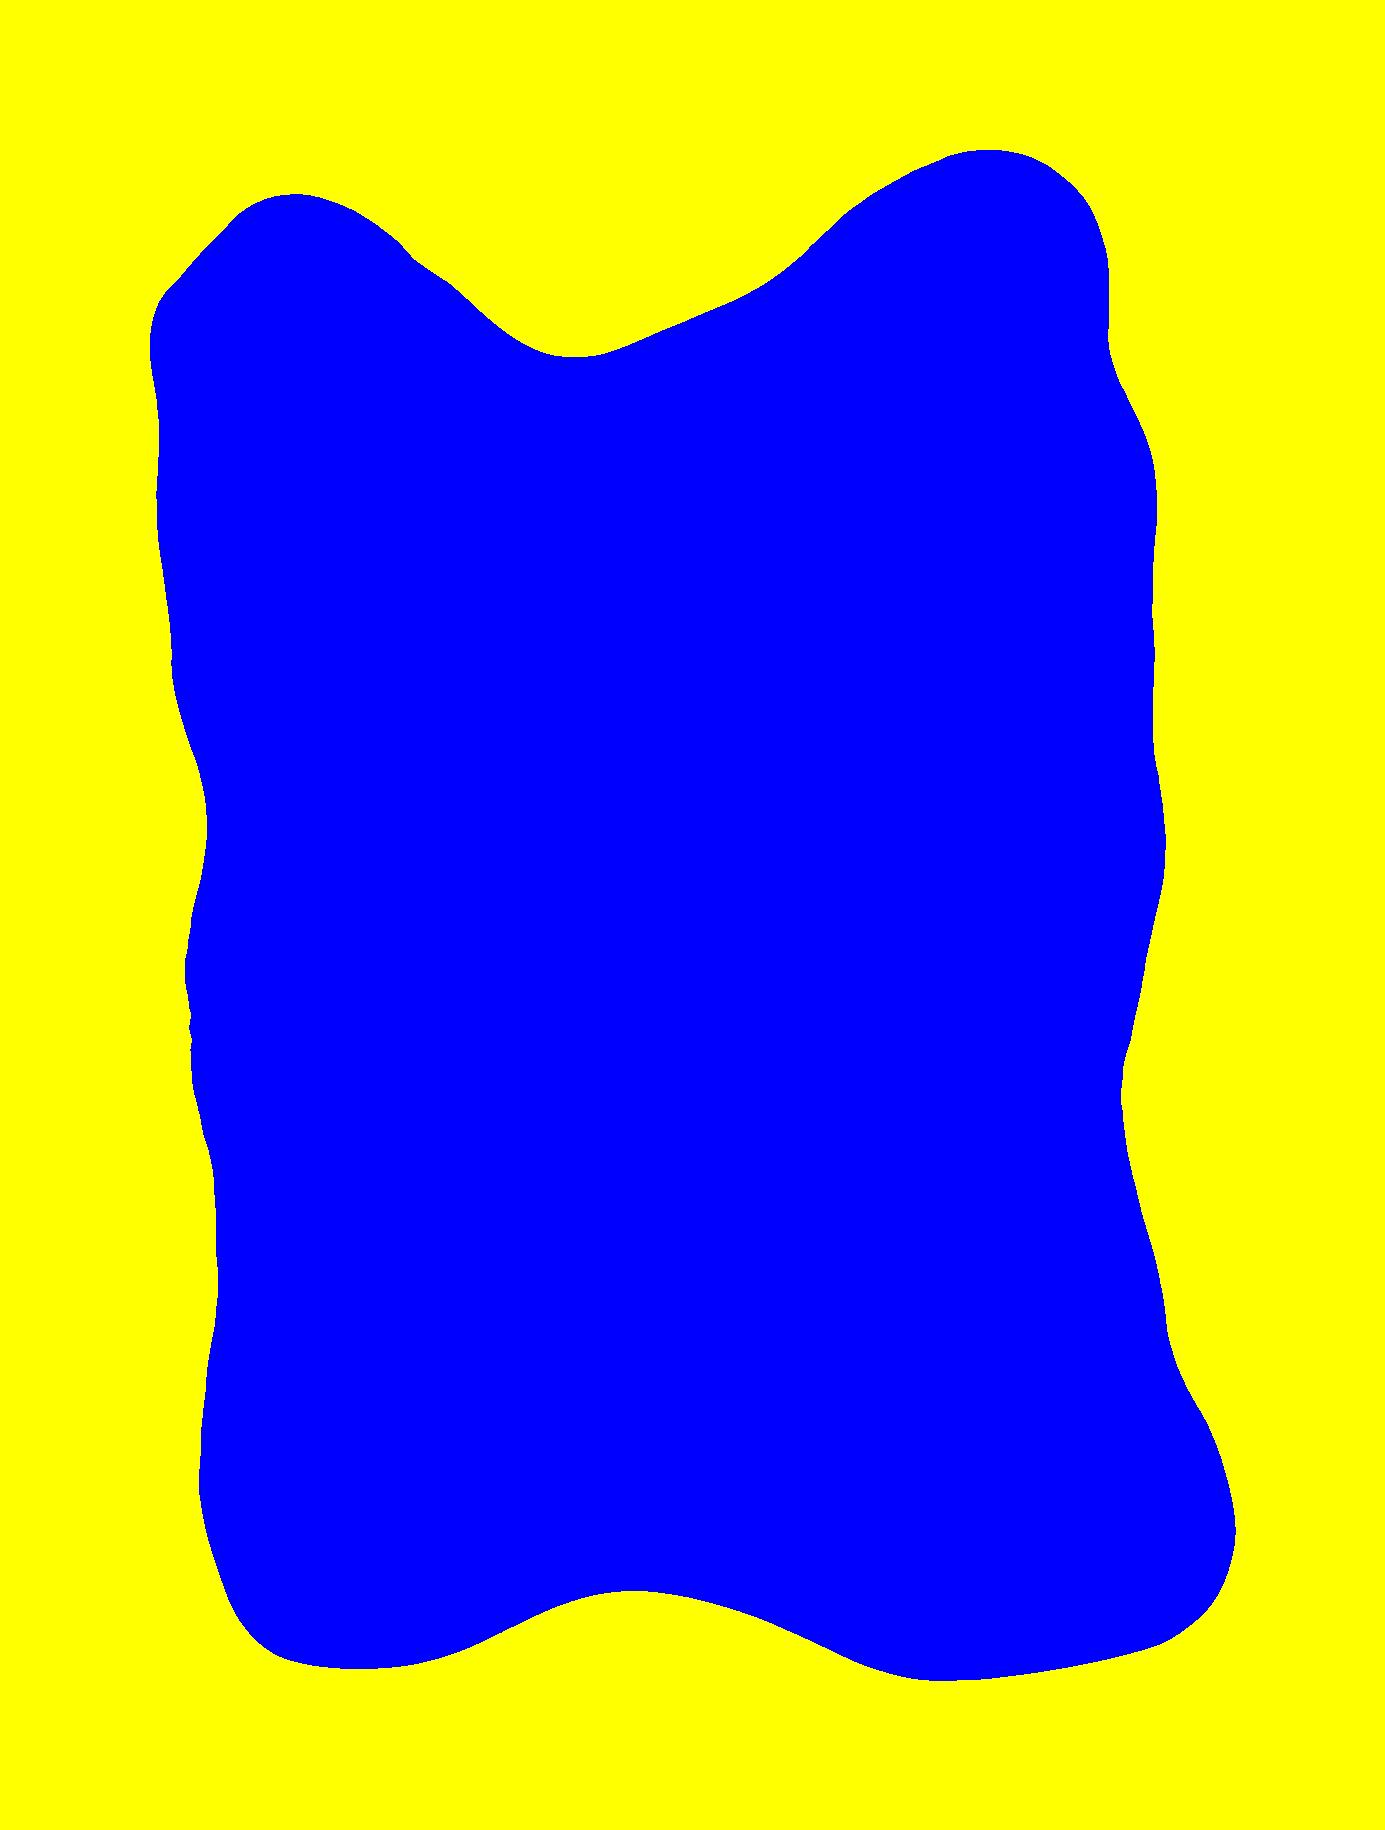
\includegraphics[width=.9\linewidth]{img/segmentation/good/watershed/segmented.jpg}
		\subcaption*{}
		\label{}
	\end{subfigure}
	\begin{subfigure}[b]{0.24\textwidth}
		\centering
		\includegraphics[width=.9\linewidth]{img/segmentation/bad/watershed/cut.jpg}
		\subcaption{}
		\label{fig:watershed-bad}
	\end{subfigure}
	\begin{subfigure}[b]{0.24\textwidth}
		\centering
		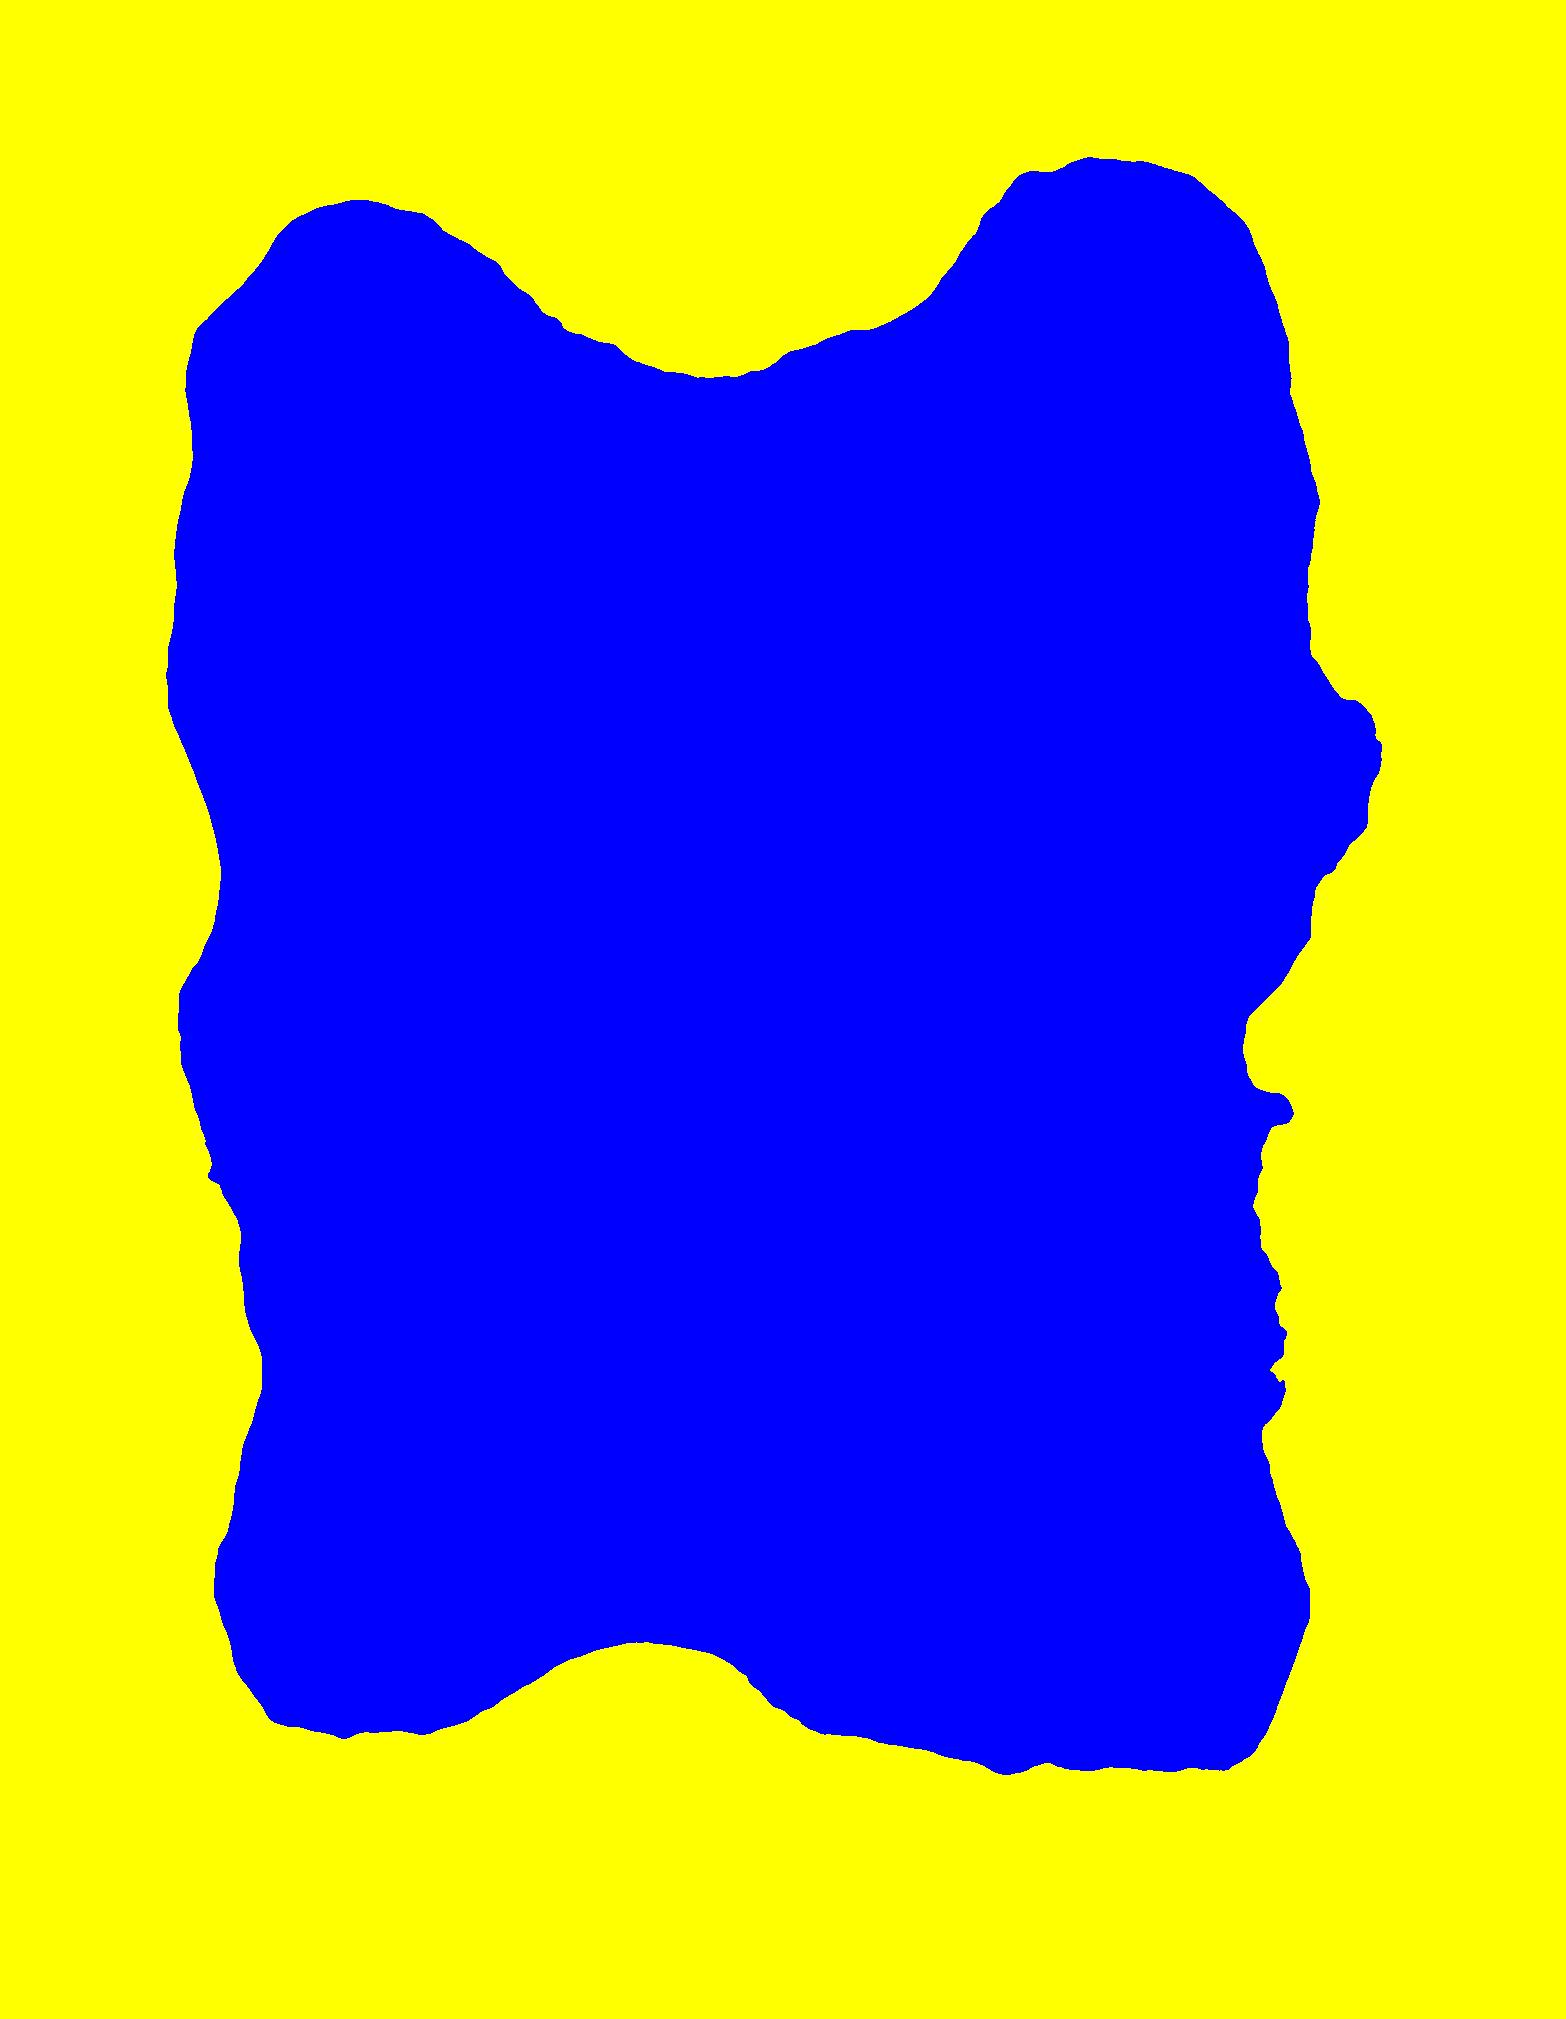
\includegraphics[width=.9\linewidth]{img/segmentation/bad/watershed/segmented.jpg}
		\subcaption*{}
		\label{}
	\end{subfigure}
	\caption{Image segmentation using watershed algorithm for two images}
	\label{fig:watershed}
\end{figure}

We chose the parameter $\mu$ as $1.25$ and used the largest resulting label as foreground pixels. While this yielded results that were sufficient to determine where the  location of the bone in the image is, the exact outline of the bone could not be reproduced using this method as visible in Figure \ref{fig:watershed-bad}. Nevertheless we leveraged this method to limit the search space for the following segmentation methods by cutting out the bounding box of the bone from the rest of the image.

\subsubsection{SLIC}

Simple linear iterative clustering (SLIC) is a method proposed by Achanta et. al. in \cite{achanta2012slic} to extract areas of perceptual similarity from an image. While this is not a texture based method, by clustering the image into small regions of the same size we hoped to adhere to the edges of the bone. SLIC employs k-means clustering representing each pixel by its color values in the CIELAB color space and its position in the image. The parameter $k$ is the number of desired superpixels. An additional parameter $m$ can be supplied to weigh spatial and color information in the distance function of the cluster algorithm. A small value for $m$ leads to less densely packed superpixels that adhere more tightly to boundaries.

\begin{figure}[h]
	\centering
	\begin{subfigure}[b]{0.24\textwidth}
		\centering
		\includegraphics[width=.9\linewidth]{img/segmentation/good/slic/cut.jpg}
		\subcaption{}
		\label{fig:slic:good}
	\end{subfigure}
	\begin{subfigure}[b]{0.24\textwidth}
		\centering
		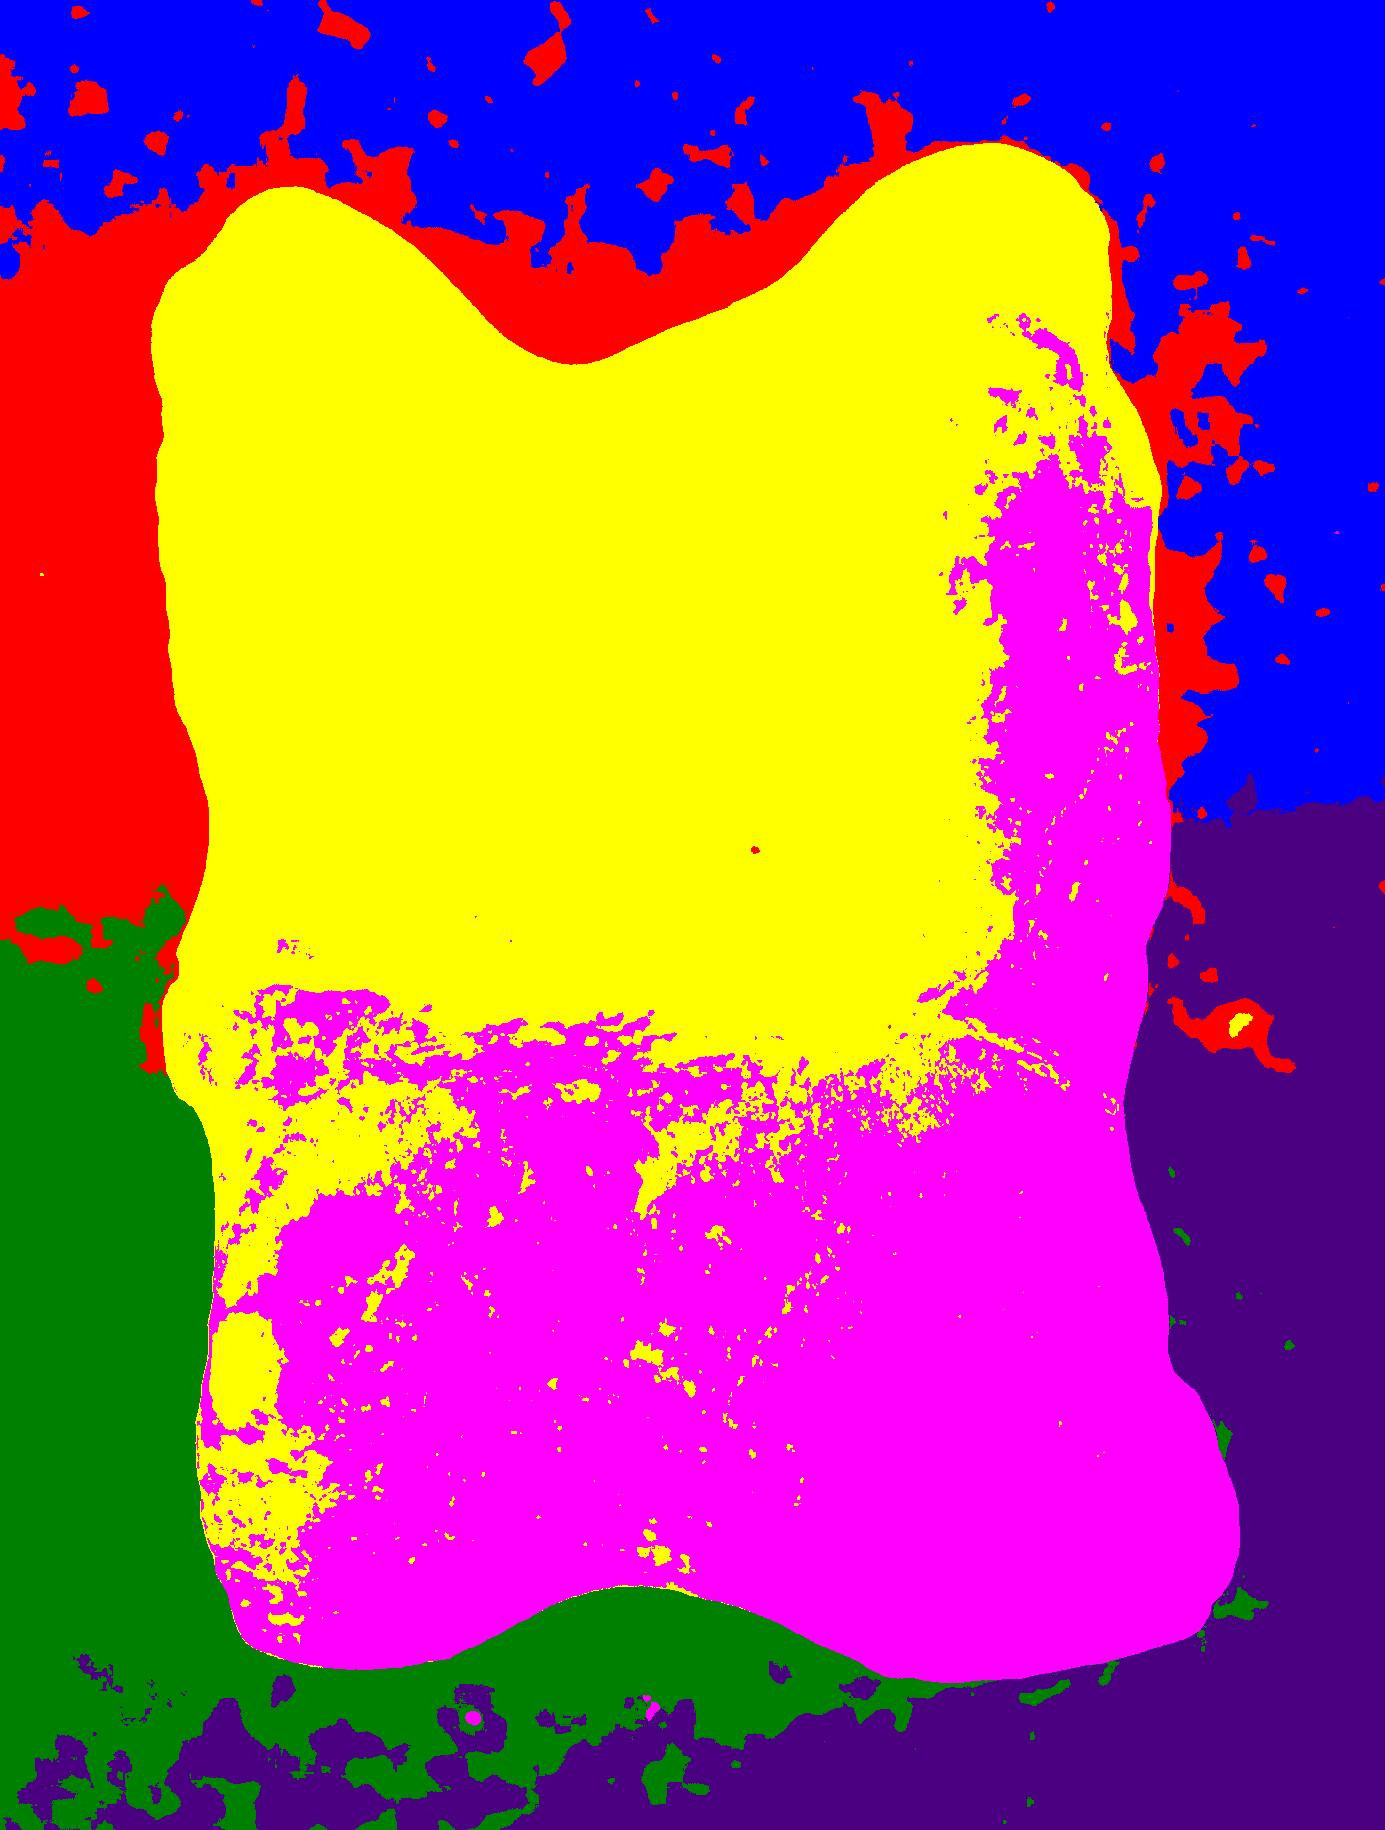
\includegraphics[width=.9\linewidth]{img/segmentation/good/slic/segmented.jpg}
		\subcaption*{}
		\label{}
	\end{subfigure}
	\begin{subfigure}[b]{0.24\textwidth}
		\centering
		\includegraphics[width=.9\linewidth]{img/segmentation/bad/slic/cut.jpg}
		\subcaption{}
		\label{fig:slic:bad}
	\end{subfigure}
	\begin{subfigure}[b]{0.24\textwidth}
		\centering
		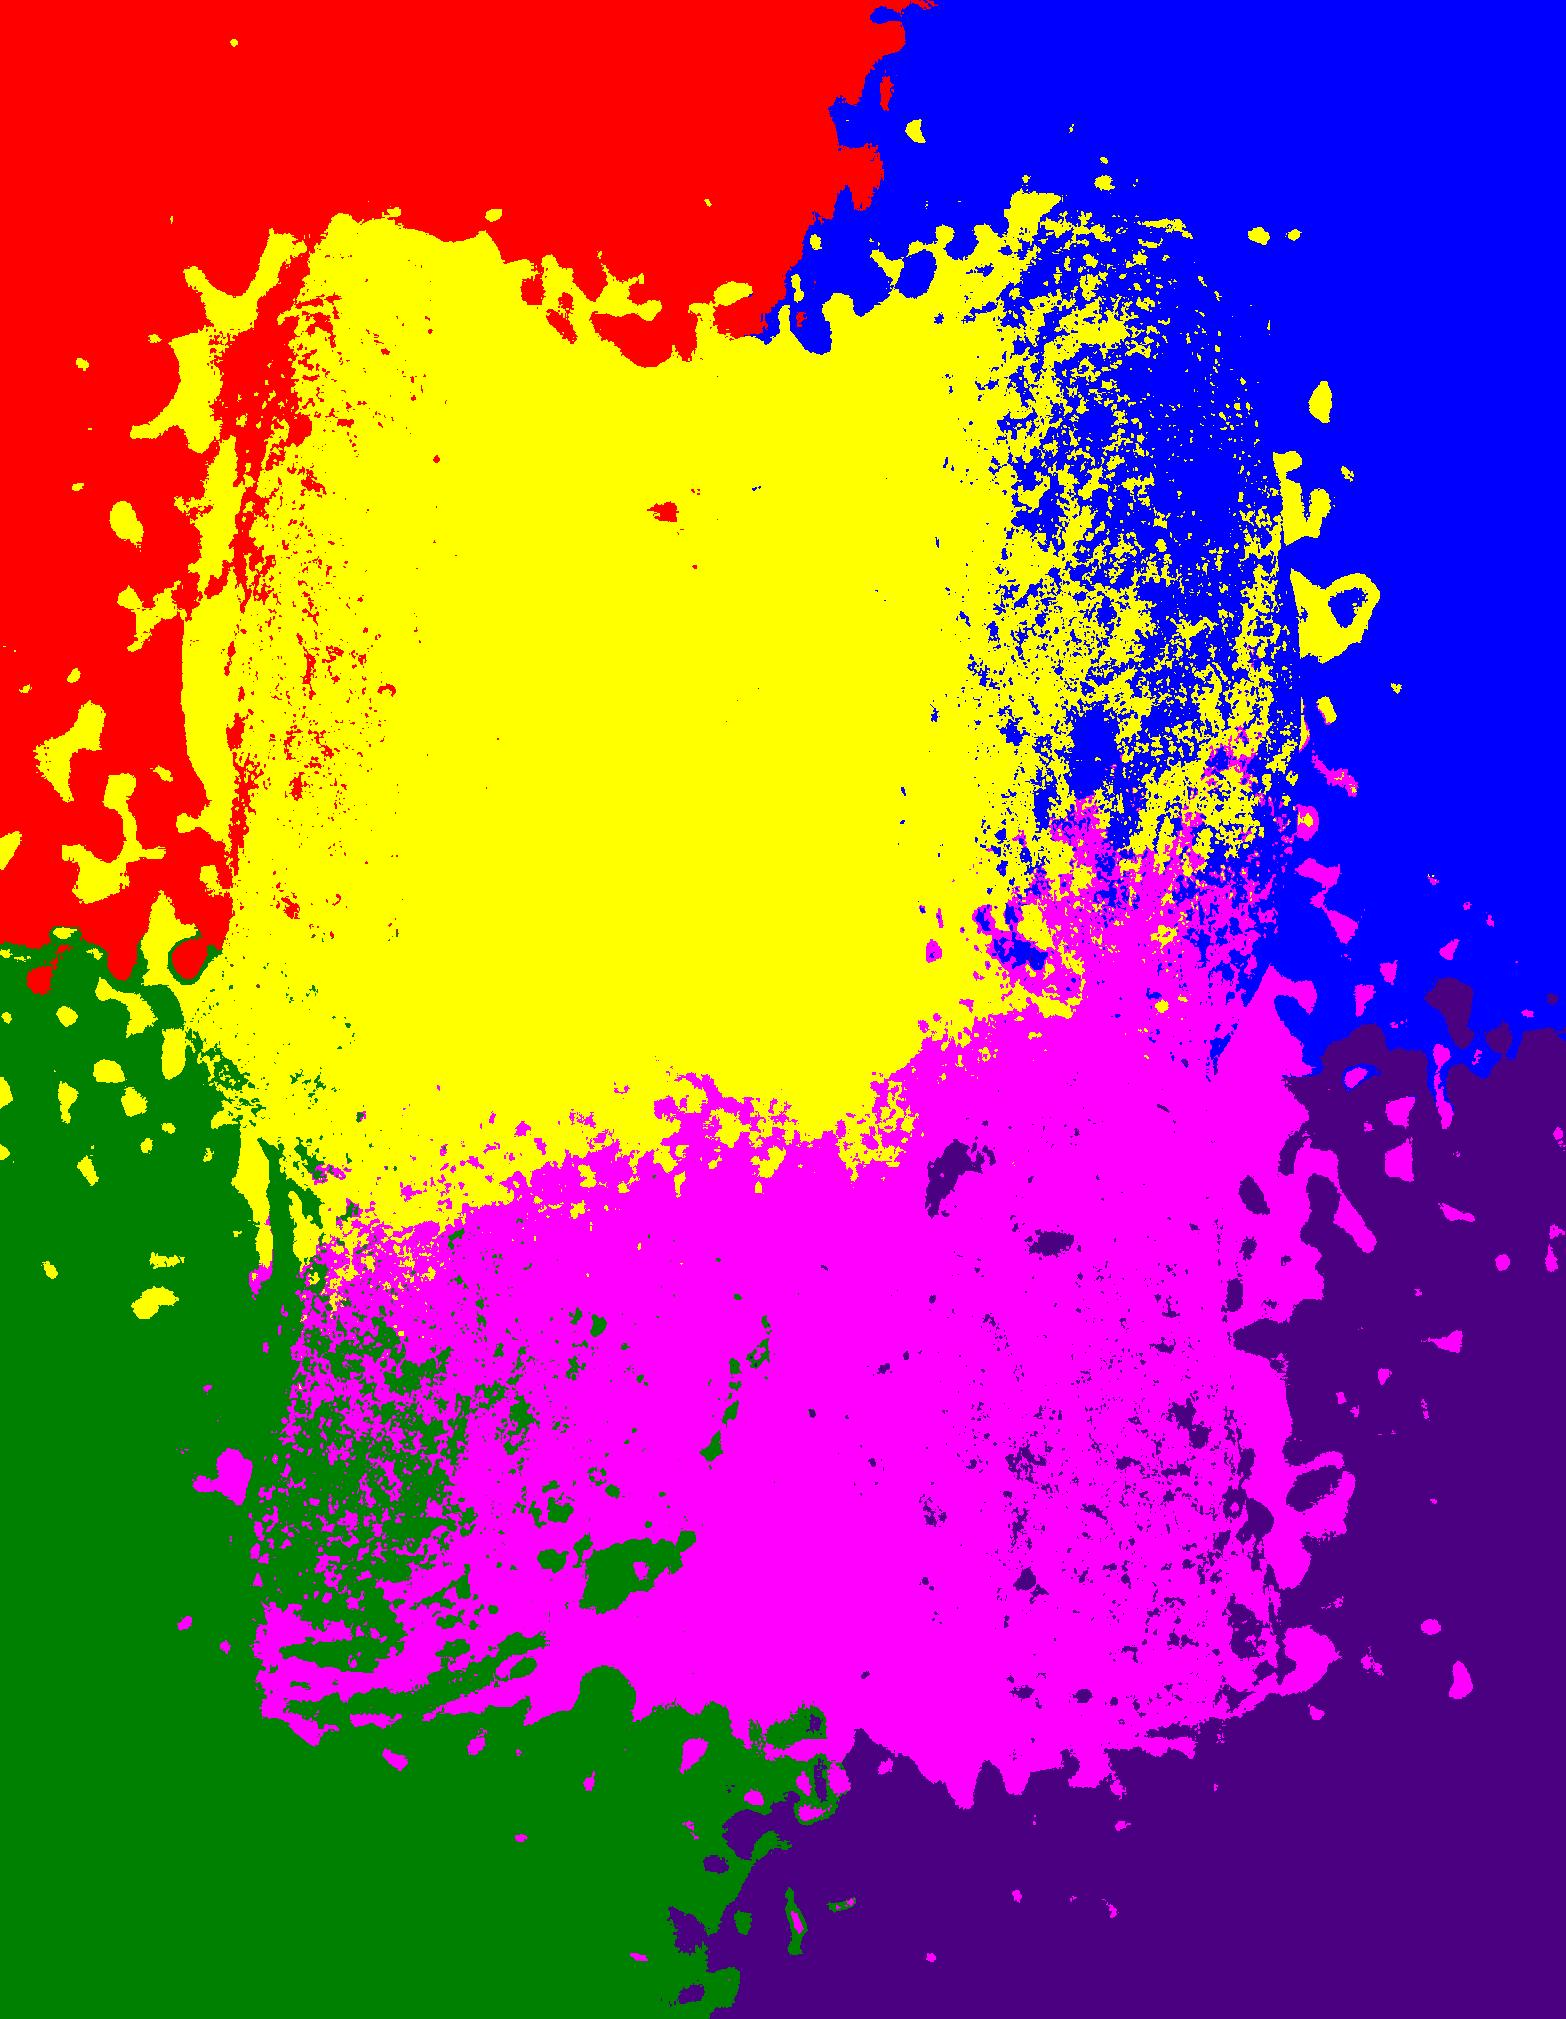
\includegraphics[width=.9\linewidth]{img/segmentation/bad/slic/segmented.jpg}
		\subcaption*{}
		\label{}
	\end{subfigure}
	\caption{Image segmentation using SLIC superpixels for two images}
	\label{fig:slic}
\end{figure}

This superpixel method works well for images with differing background and foreground colors as visible in Figure \ref{fig:slic:good} and when using a sufficiently number of superpixels $k=8$. Increasing the weight $m$ to $m=15$ leads to compact clusters that align to the bone shape. When background and foreground colors are similar as it is the case in Figure \ref{fig:slic:bad}, the clusters become more frayed and do not always align anymore with the bone shape.

\subsubsection{Felzenszwalb Graph-Based}

The method proposed by Felzenszwalb et. al in \cite{felzenszwalb2004efficient} is a graph based image segmentation method that works with the local neighborhoods of pixels. We decided to implement this method because it tries to segment perceptually similar regions. It works on the neighborhood graph of the image and defines the edges weights as the difference between the intensity of the pixels. The algorithm then iteratively splits and merges segments of the graph until the overall segmentation obeys certain global properties. The global properties are that the segmentation is neither too fine nor too coarse.

\begin{itemize}
	\item A segmentation $S$ is too fine if there is some pair of regions $C_1, C_2 \in S$ for which there is no evidence of a boundary between them
	\item A segmentation $S$ is too coarse when there exists a proper refinement of $S$ that is not too fine
\end{itemize}

The split algorithm can be configured by a parameter $k$, which sets the scale of observation. A larger $k$ means that stronger evidence for a boundary is needed to perform a split.

\begin{figure}[h]
	\centering
	\begin{subfigure}[b]{0.24\textwidth}
		\centering
		\includegraphics[width=.9\linewidth]{img/segmentation/good/felzenszwalb/cut.jpg}
		\subcaption{}
		\label{fig:felzenszwalb:good}
	\end{subfigure}
	\begin{subfigure}[b]{0.24\textwidth}
		\centering
		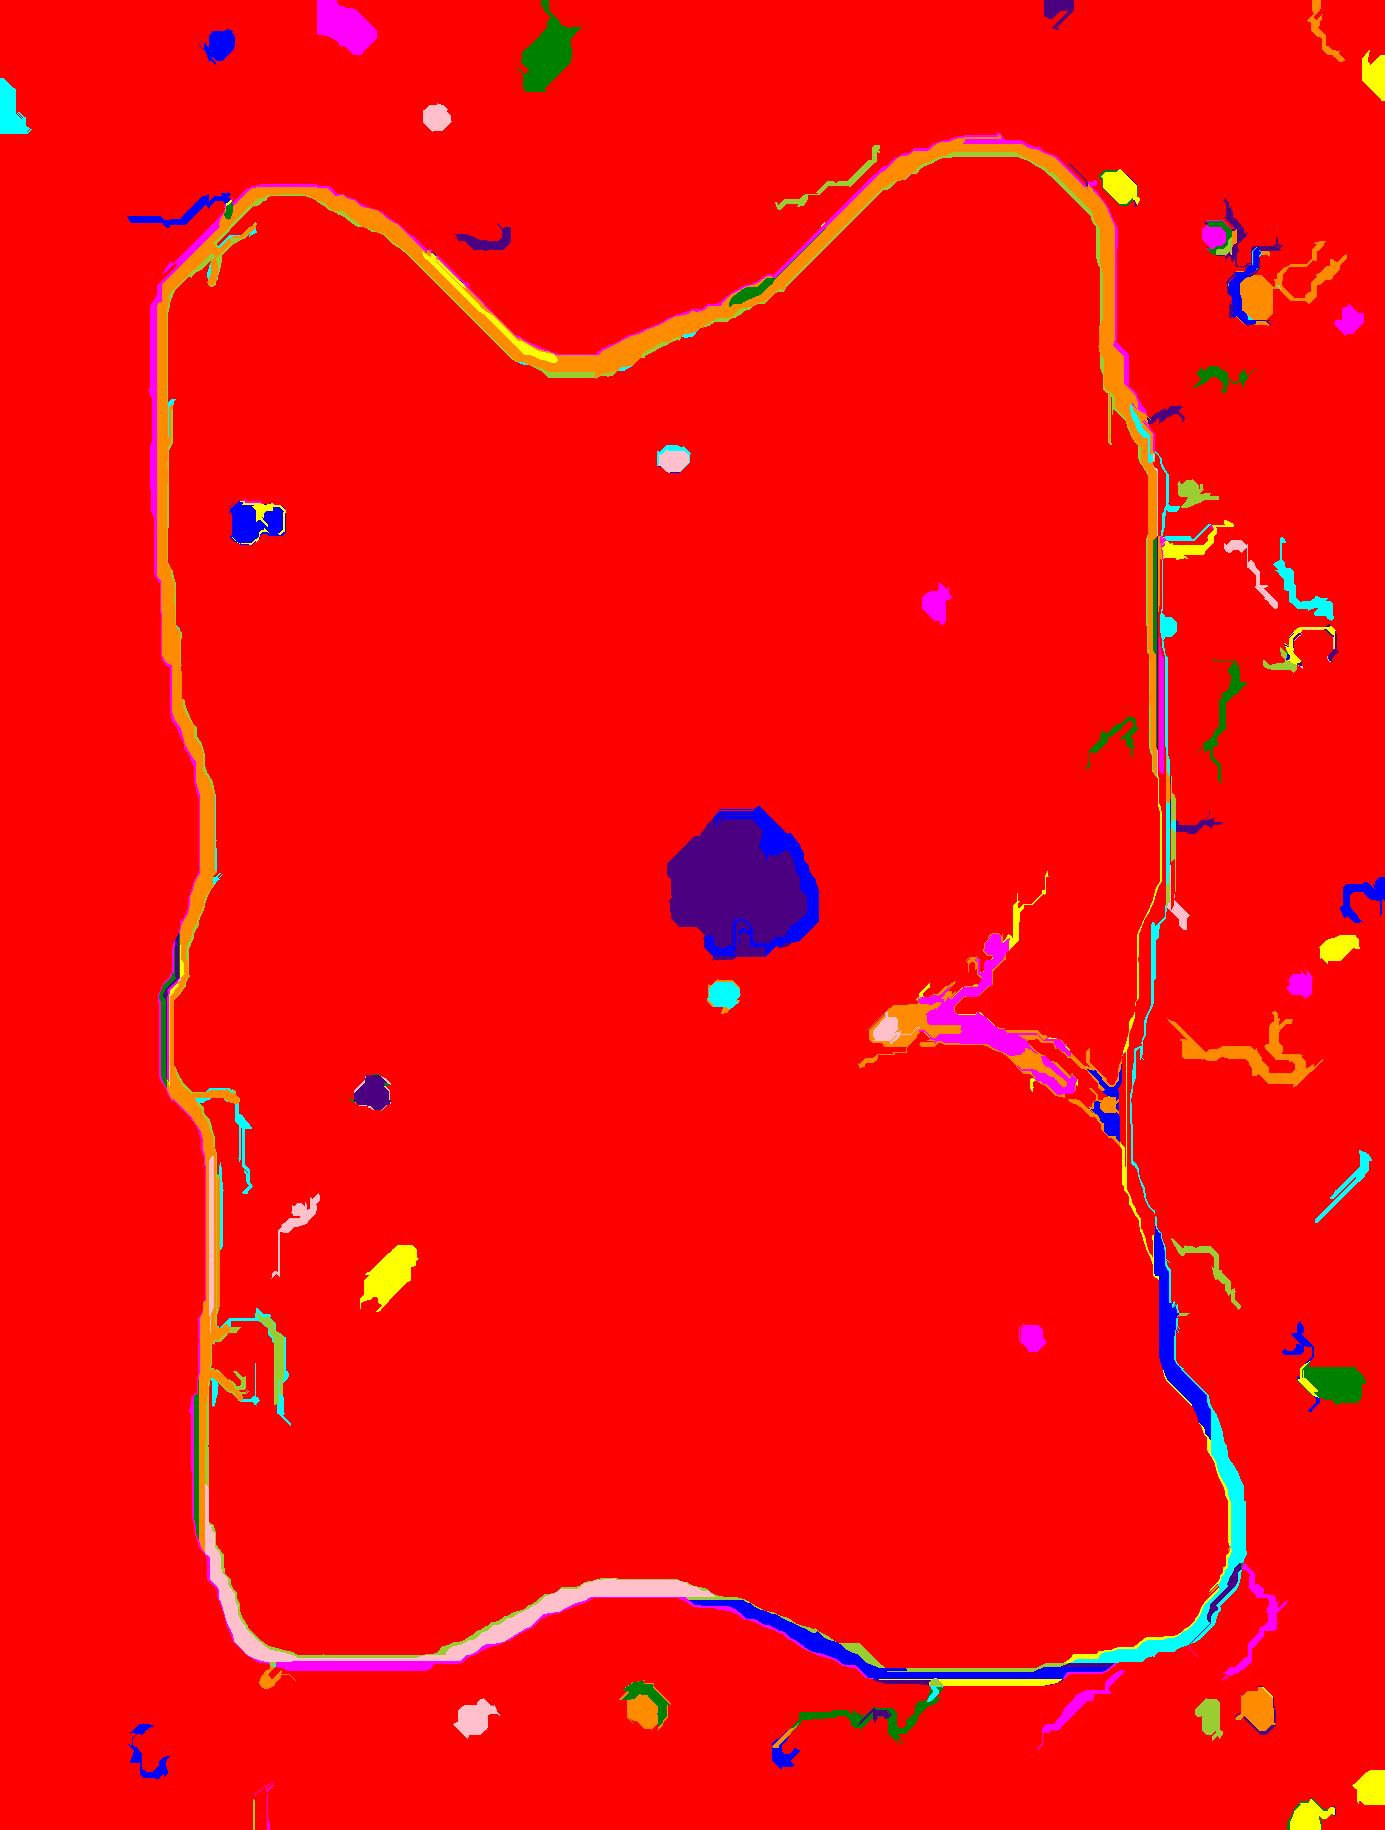
\includegraphics[width=.9\linewidth]{img/segmentation/good/felzenszwalb/segmented.jpg}
		\subcaption*{}
		\label{}
	\end{subfigure}
	\begin{subfigure}[b]{0.24\textwidth}
		\centering
		\includegraphics[width=.9\linewidth]{img/segmentation/bad/felzenszwalb/cut.jpg}
		\subcaption{}
		\label{fig:felzenszwalb:bad}
	\end{subfigure}
	\begin{subfigure}[b]{0.24\textwidth}
		\centering
		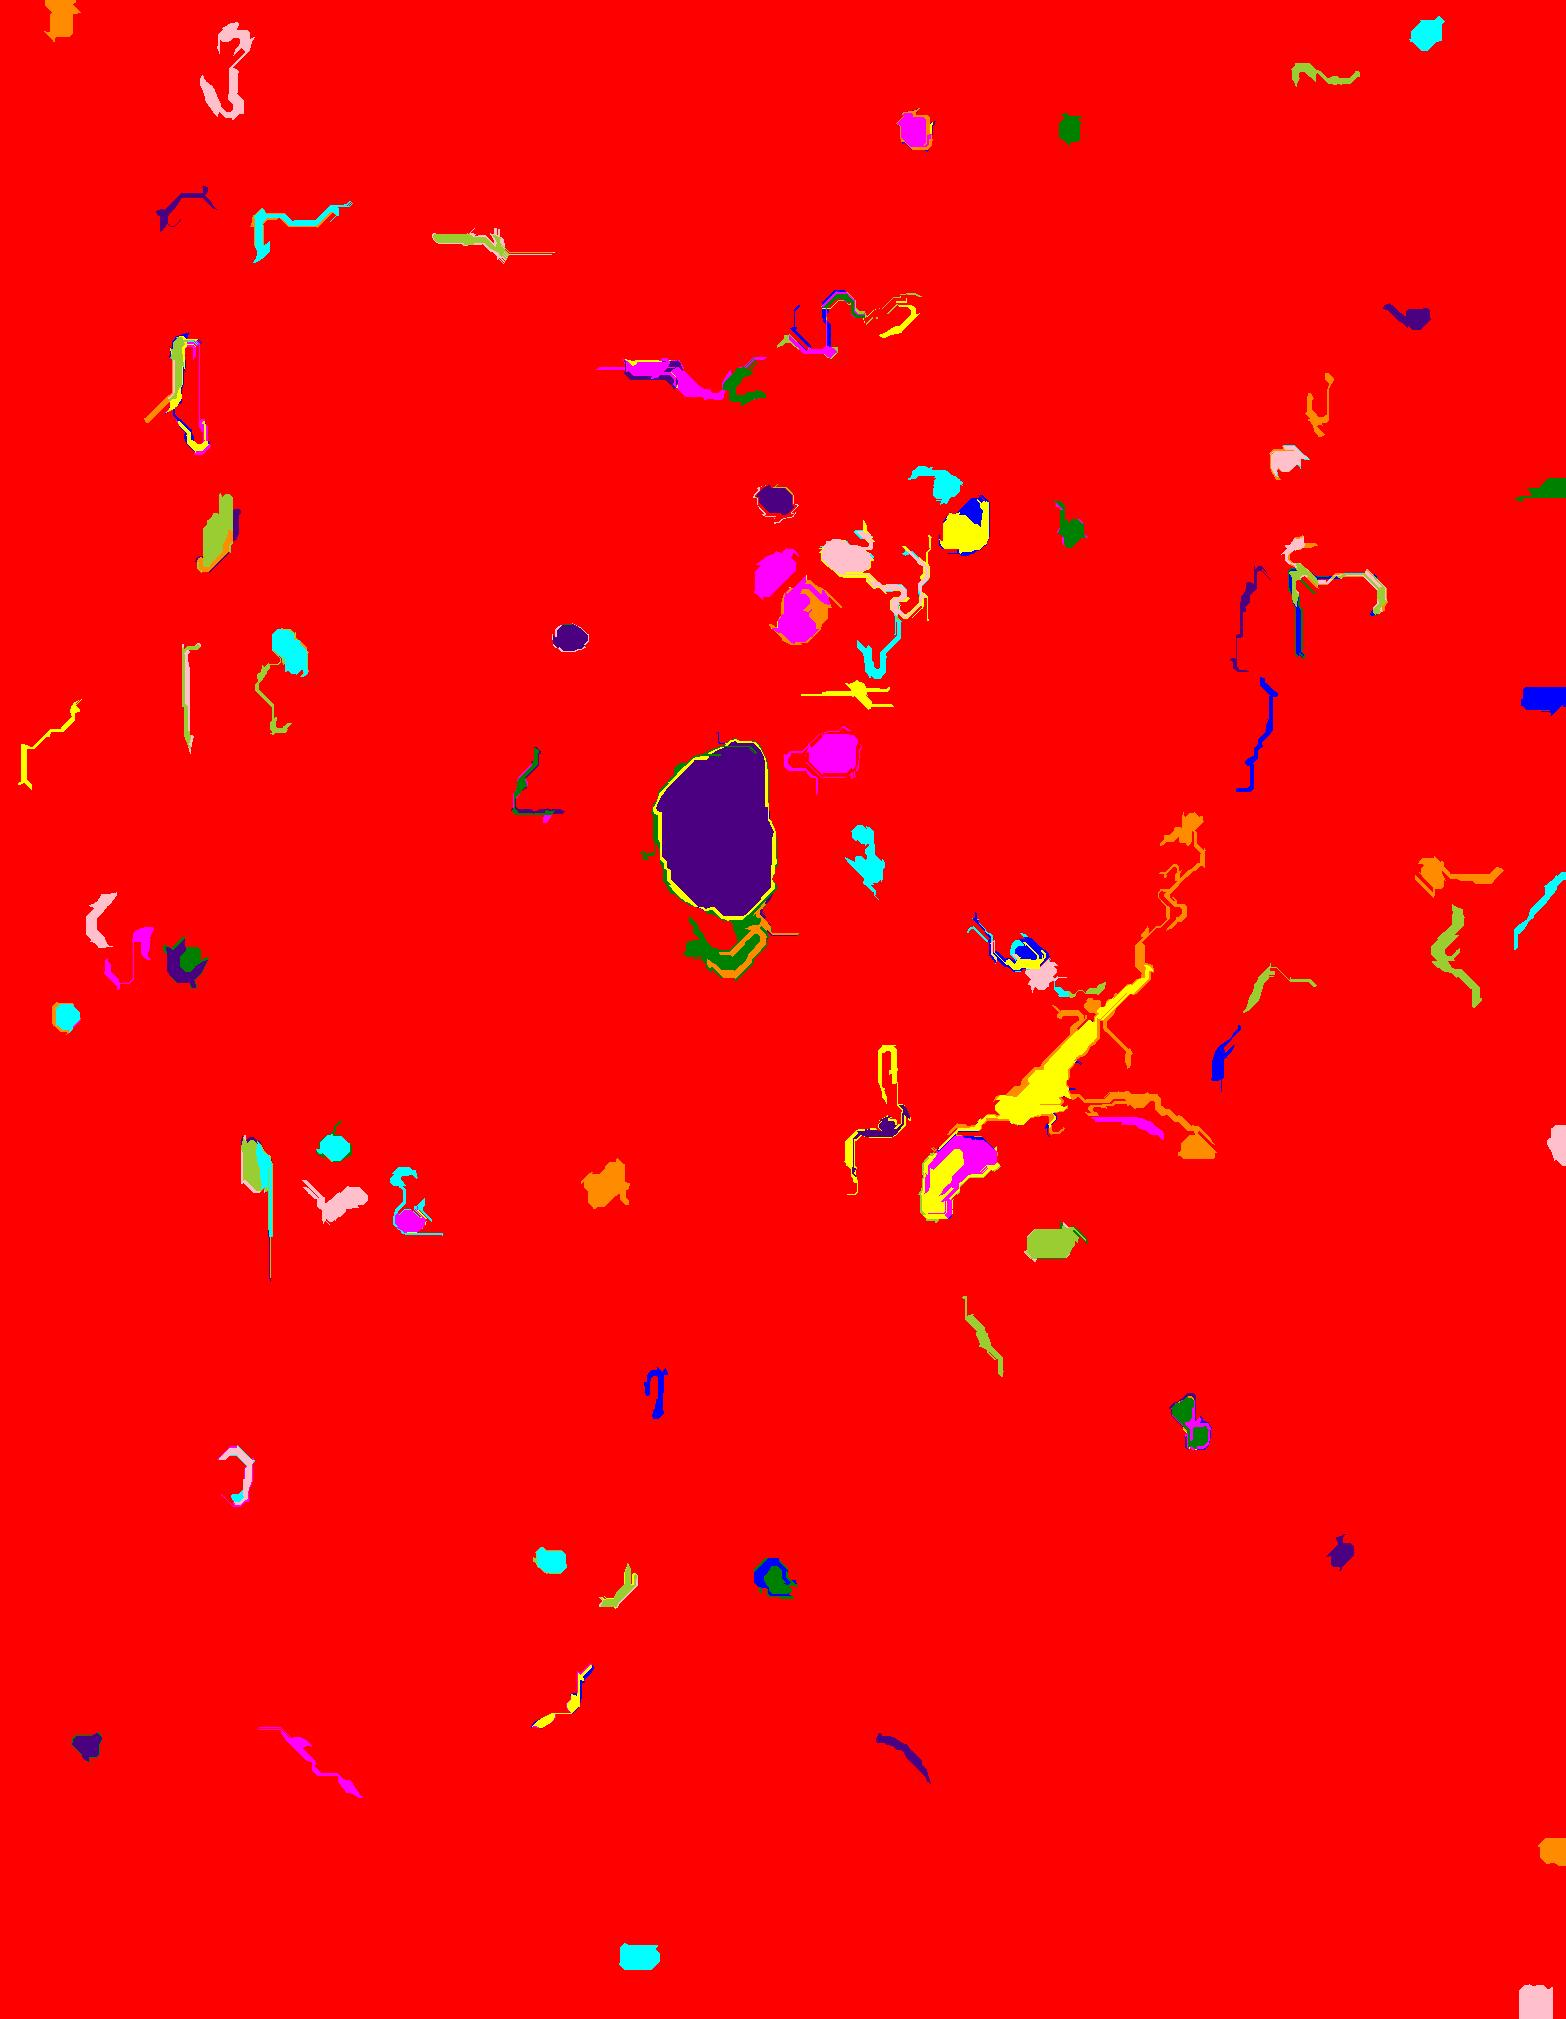
\includegraphics[width=.9\linewidth]{img/segmentation/bad/felzenszwalb/segmented.jpg}
		\subcaption*{}
		\label{}
	\end{subfigure}
	\caption{Image segmentation using Felzenszwalb's graph-based method for two images}
	\label{fig:felzenszwalb}
\end{figure}

The labels generated by Felzenszwalb's method adhere to the edges of the bone, but some additional areas are included in the result as well. The number of labels is not selectable and for large images this method can create hundreds of labels, which complicates label selection for the user, so a sufficiently high observation level $k$ needs to be chosen to reduce the number of labels. For our purpose, we chose $k=1000$. The images that are difficult to segment could often not be correctly segmented using this method as visible in Figure \ref{fig:felzenszwalb:bad}. When choosing a small value for $k$ a huge amount of small labels was generated. On the other hand, when choosing a large value for $k$, the bone and background collapsed into a single label.

\subsubsection{Gabor Filters}

Another way to do texture segmentation in images is to represent the image using Gabor filters. The image is decomposed using Gabor filters into a number of filtered images that each contain variations in intensity over a certain frequency and in a certain direction. To obtain filtered images for segmentation it is necessary to define the parameters of the filters well. We used the filter selection method from \cite{jain1990unsupervised} to obtain the filter parameters. Gabor filters are tailored to represent the early stages of the human visual system, so the image is preprocessed using a non-linear function first and then the filters with the selected parameters are applied. This results in an vector of pixel values per pixel that can be clustered using k-means.

\begin{figure}[h]
	\centering
	\begin{subfigure}[b]{0.24\textwidth}
		\centering
		\includegraphics[width=.9\linewidth]{img/segmentation/good/gabor/cut.jpg}
		\subcaption{}
		\label{fig:gabor:good}
	\end{subfigure}
	\begin{subfigure}[b]{0.24\textwidth}
		\centering
		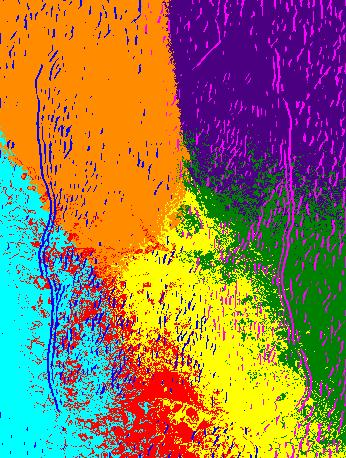
\includegraphics[width=.9\linewidth]{img/segmentation/good/gabor/segmented.jpg}
		\subcaption*{}
		\label{}
	\end{subfigure}
	\begin{subfigure}[b]{0.24\textwidth}
		\centering
		\includegraphics[width=.9\linewidth]{img/segmentation/bad/gabor/cut.jpg}
		\subcaption{}
		\label{fig:gabor:bad}
	\end{subfigure}
	\begin{subfigure}[b]{0.24\textwidth}
		\centering
		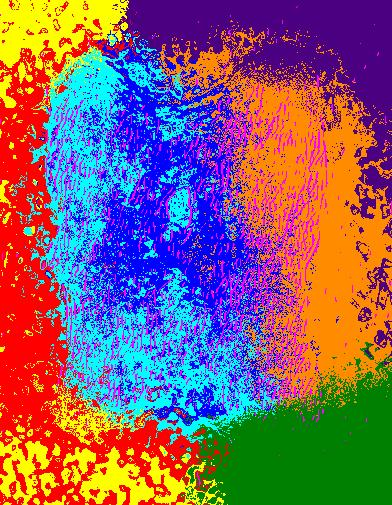
\includegraphics[width=.9\linewidth]{img/segmentation/bad/gabor/segmented.jpg}
		\subcaption*{}
		\label{}
	\end{subfigure}
	\caption{Image segmentation using Gabor filters for two images}
	\label{fig:gabor}
\end{figure}

The results of clustering the Gabor filter features vary heavily depending on the image. For almost all images, wavy features either in the background or on the bone are detected. Depending on where they are detected, one of these labels can be used to outline the bone. As visible in Figure \ref{fig:gabor} this sometimes works better for difficultly separable images.

\subsubsection{Textural Edge Detection}

An approach to edge detection using semi-local texture features was also implemented. Since it wasn't necessary to segment the whole bone as foreground pixels but only the outline, we defined the outline as a region where there are different textures on either side. To detect vertical and horizontal edges we considered the local neighborhood of $n$ pixels into each direction of the pixel $N_{left}(x,y), N_{right}(x,y), N_{top}(x,y), N_{bottom}(x,y)$.

\begin{equation}
\begin{split}
	& N_{left}(x,y) = \{ (x-n,y), (x-1,y) \} \\
	& N_{right}(x,y) = \{ (x+1,y), (x+n,y) \} \\
	& N_{top}(x,y) = \{ (x,y+n), (x,y+1) \} \\
	& N_{bottom}(x,y) = \{ (x,y-1), (x,y-n) \}
\end{split}
\end{equation}

We then calculated textural features $F$ for these local neighborhoods and used the distance between them as a measure for an edge. For this purpose we used Haralick textural features \cite{haralick1973textural} or parameter free threshold adjacency statistics \cite{hamilton2007fast} as feature extraction function $\vec{b}$.  

\begin{equation}
f(x,y) = \left( \begin{array}{c}
\vec{b}(N_{left}(x,y)) - \vec{b}(N_{right}(x,y)) \\
\vec{b}(N_{top}(x,y)) - \vec{b}(N_{bottom}(x,y)
\end{array} \right)
\end{equation}

\begin{figure}[h]
	\centering
	\begin{subfigure}[b]{0.24\textwidth}
		\centering
		\includegraphics[width=.9\linewidth]{img/segmentation/good/textural-edges/cut.jpg}
		\subcaption{}
		\label{fig:textural:good}
	\end{subfigure}
	\begin{subfigure}[b]{0.24\textwidth}
		\centering
		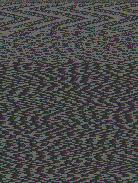
\includegraphics[width=.9\linewidth]{img/segmentation/good/textural-edges/segmented.jpg}
		\subcaption*{}
		\label{}
	\end{subfigure}
	\begin{subfigure}[b]{0.24\textwidth}
		\centering
		\includegraphics[width=.9\linewidth]{img/segmentation/bad/textural-edges/cut.jpg}
		\subcaption{}
		\label{fig:textural:bad}
	\end{subfigure}
	\begin{subfigure}[b]{0.24\textwidth}
		\centering
		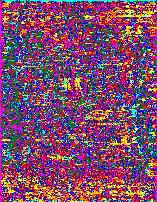
\includegraphics[width=.9\linewidth]{img/segmentation/bad/textural-edges/segmented.jpg}
		\subcaption*{}
		\label{}
	\end{subfigure}
	\caption{Image segmentation using textural edge detection for two images}
	\label{fig:textural}
\end{figure}

The results for this segmentation method were mixed as well. While edges are detected correctly on images with high contrast as visible in Figure \ref{fig:textural:good}, the results appear random for images with low contrast between bone and background as shown in Figure \ref{fig:textural:bad}. Some structure is visible in Figure \ref{fig:textural:bad}, but the clustering does not work well in this case, probably because of the low number of features.

\subsection{Triangulation and Outlining}

The next step for preprocessing images was extracting the outline from a segmented image. As stated in Section
\ref{sub:segmentation}, we marked some pixels in the images as being pixels that lie on the bone.
To extract the outline from these pixels, we first transformed them into points in the x-y-space and then
triangulated them using the Delaunay triangulation.

To reduce the number of outliers that were detected as foreground pixels,
we decided to use the DBSCAN algorithm from \cite{ester1996density} and apply density based clustering to the points
beforehand. DBSCAN allowed us to create clusters from the data, which correspond to closely packed points. Since
the points on the bone were closely packed, and the points not on the bone were only sparsely detected as
foreground pixels this allowed us to filter some of the false-positives. Another benefit of the DBSCAN algorithm is that,
by defining our bone as a large densely connected area, we were able to use the largest cluster from the result,
so closely packed areas that are disconnected from the bone were also removed.

The Delaunay triangulation was applied to the remaining points to create a triangulated mesh. Since Delaunay
triangulation can only create meshes with convex outlines, another step was required to extract the bone outline
from the triangulation. For this purpose we used the $\alpha$-complex of the mesh as defined in \cite{akkirajualpha}.
The $\alpha$-complex algorithm removes outer triangles for the Delaunay triangulation that have a radius which exceeds
$\frac{1}{\alpha}$. $\alpha$ is a parameter and was chosen as $25$ for our purpose, which provided us with
an accurate concave outline of the bone.

Since we are analyzing the shape of the object, a manual step was introduced here to give the user the ability to
approve the automatically extracted outline and adapt it if the result was not satisfactory. We gave the user the
ability to mark pixels as foreground/background as well as fill a rectangle with a grid of foreground or background pixels.
This allows the user to easily adapt a triangulation and, if necessary, create a completely new one. It becomes
especially important because difficulties with the image segmentation algorithms.

Since the bones might have different sizes and positions, due to different image sizes and position of the bone in
the image, we needed to introduce another normalization step afterwards. We decided to remove all variance in between the bones that are not attributed to shape. For this purpose we executed the first two steps of Procrustes
analysis, also used in Section \ref{subsub:procrustes}.

\begin{itemize}
	\item Transformation of all point sets into the coordinate center
	\begin{equation}
		\begin{split}
			& \vec{\mu}_x = \frac{1}{n} \sum_{\vec{x} \in X} \vec{x} \\
			& X_c = \{ \vec{x} - \vec{\mu}_x \mid \vec{x} \in X \}
		\end{split} 
	\end{equation}
	\item Scaling all point sets uniformly
	\begin{equation}
		\begin{split}
			& s = \sqrt{\frac{\sum\limits_{\vec{x} \in X_c}||\vec{x}||^2}{n}} \\
			& X_s = \left\{ \frac{\vec{x}}{s} \mid \vec{x} \in X_c \right\}
		\end{split}
	\end{equation}
\end{itemize}

To represent the outlines we decided to use splines as introduced in Section \ref{section:splines},
as this allows us to easily extract segments of the bone outline. After the normalization all outlines
adhere to the following standards.

\begin{itemize}
	\item The centroid lies close to the coordinate center $(0,0)$
	\item The expansion lies within the ranges of $0$ to $2$ in the x and y directions
\end{itemize}

To have consistent spline representations, which all start at $s_y(0) = 0$, we calculated the intersection between the x-axis and the bone outline
in the positive section of the x-axis. This point was introduced as the starting point for the polygon that is our outline.
The spline $(s_x(t), s_y(t))$ for the interval $t \in [0, 1]$ was then extracted leading to the
following standards for the spline representation for each bone. These standards can be leveraged for the comparison algorithm.

\begin{equation}
\begin{split}
& s_y(0) = 0 \\
& s_y(1) = 0 \\
& s_x^\prime(0) = s_x^\prime(1) \\
& s_y^\prime(0) = s_y^\prime(1)
\end{split}
\end{equation}

\subsection{Landmark Extraction}
\label{sub:landmarks}

As some of the features we propose in this work are landmark based, and the detection of on-site-measurable differences
is based on landmarks as well, a method to extract these landmarks from the outline of the bone is needed. In contrast to
our approach, former work on the talus by zooarcheologists was based on manually located landmarks that correspond to
biological features of the bone. Since our goal was to automate the process as much as possible and some of the landmarks
are not positioned on the outline of the bone, using them was not feasible in our case. We selected landmarks on the outline
of the bone that could be located automatically and overlap as much as possible with the landmark definitions by the
zooarcheologists. For this purpose we introduced two methods that extract landmarks from outlines of Tali. The landmarks
found by these methods have very similar positions but differ in on-site-measurability and stability in-between classes.

\begin{figure}
	\centering
	\begin{subfigure}[b]{0.3\textwidth}
		\centering
		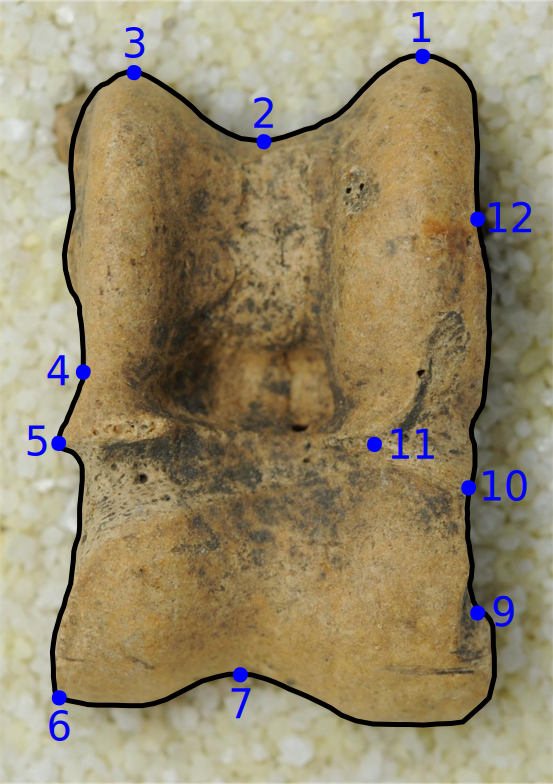
\includegraphics[width=.9\linewidth]{img/landmarks/manual.pdf}
		\subcaption{Manual}
	\end{subfigure}
	\begin{subfigure}[b]{0.3\textwidth}
		\centering
		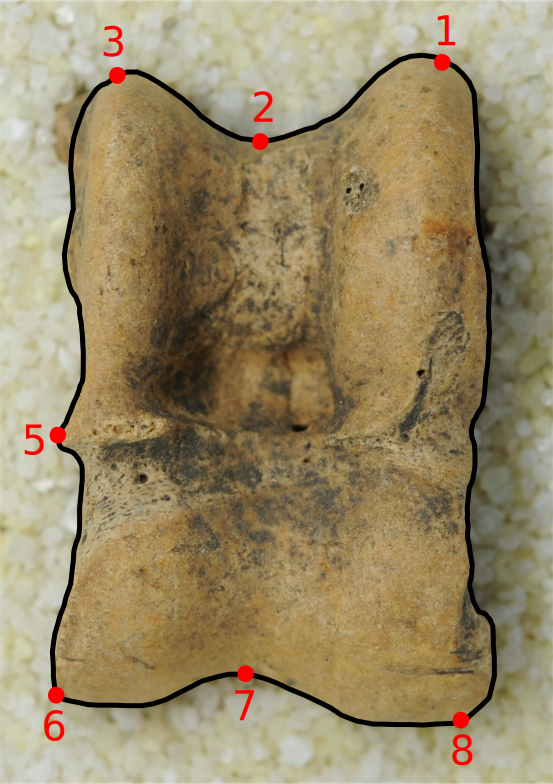
\includegraphics[width=.9\linewidth]{img/landmarks/angles.pdf}
		\subcaption{By angle}
	\end{subfigure}
	\begin{subfigure}[b]{0.3\textwidth}
		\centering
		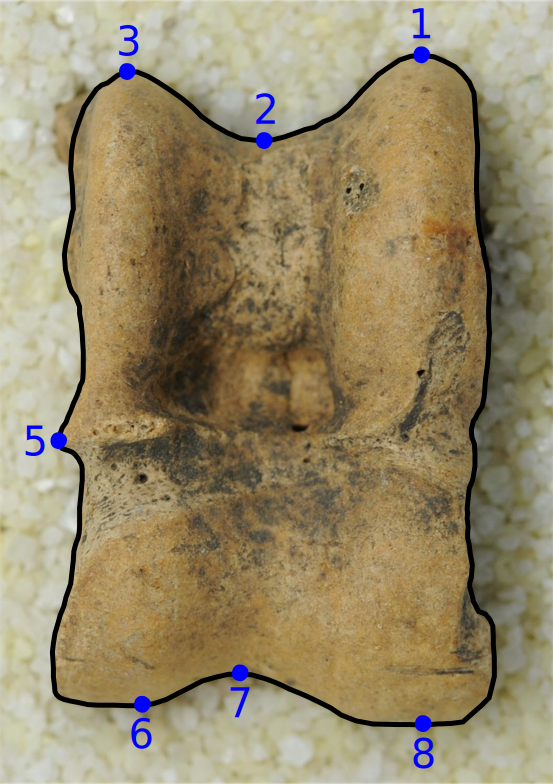
\includegraphics[width=.9\linewidth]{img/landmarks/space-partitioning.pdf}
		\subcaption{By space partitioning}
	\end{subfigure}
	\caption{Landmarks by method}
	\label{fig:landmark-methods}
\end{figure}

Figure \ref{fig:landmark-methods} shows the results of the three landmark locating methods: manual selection, extraction by angles and
by space partitioning. The biological correspondences of the landmarks are as follows.

\begin{itemize}
\item Landmark 1: Highest point on the lateral crest
\item Landmark 2: Lowest point in between the crests
\item Landmark 3: Highest point on the medial crest
\item Landmark 4: Intersection between the medial outer edge and the medially arcing edge of the medial crest
\item Landmark 5: Out most point on the medial apex
\item Landmark 6: Lowest point on the medial outer edge
\item Landmark 7: Highest point on the distal depression
\item Landmark 9: Intersection of the distal articular surface with the Calcaneus
\item Landmark 10: Lateral end point of the lower muscle attachment line
\item Landmark 11: Intersection of the two muscle attachment lines
\item Landmark 12: Proximal end point of the lateral protrusion on the lateral crest
\end{itemize}

The landmarks that were extracted automatically are landmarks 1, 2, 3, 5, 6, 7. Furthermore we introduced the new
landmark number 8, which has no biological correspondence, but can be located robustly on all bone outlines. This newly introduced landmark can be seen in the bottom right Figures \ref{fig:landmark-methods}.

\subsubsection{Extraction by Angle}

When extracting a landmark by angle, the landmark position is defined by a minimum angle $\alpha_{min}$, a maximum
angle $\alpha_{max}$ and the information whether it is located on a minimum or a maximum turning point.
The minimum/maximum turning angle $\alpha_{t}$ between $\alpha_{min}$ and $\alpha_{max}$ of the following function
is calculated, where $\vec{i}(\alpha)$ is the intersection between a ray from the coordinate center with the angle $\alpha$ and
the outline. $\vec{i}(\alpha_t)$ is then used as the landmark.

\begin{equation}
d(\alpha) = ||\vec{i}(\alpha)||
\end{equation}

The definitions for all landmarks when using this method can be found in Appendix \ref{appendix:table:landmarks-angle}.

The landmarks found by this method are robustly located across all classes, but have a distinct disadvantage. They are
not as easily located by hand since they dont lie exactly on the high points of the outline, but slightly beneath
them  as seen in Figure \ref{fig:landmark-methods}. This makes distances in between landmarks harder to measure, which
will become relevant in Chapter \ref{chapter:measurable-differences}.

\subsubsection{Extraction by Space Partitioning}

When extracting a landmark by space partitioning, the landmark position is defined by a rectangle in which the landmark
lies, the information whether it lies on a maximum or a minimum turning point and the coordinate axis on which the
turning point lies. The rectangle is defined by $x_{min}$, $x_{max}$, $y_{min}$ and $y_{max}$. The turning point
is then found by only evaluating the respective axis inside the rectangle. The following function for turning points
is then evaluated inside the rectangle, where $s_y(x)$ is the x-coordinate of the spline at the x-coordinate $x$.

\begin{equation}
d(x) = s_y(x)
\end{equation}

The definitions for all landmarks when using the space-partitioning method can be found in Appendix
\ref{appendix:table:landmarks-space}.

When looking at the landmarks found by this method, they tend to lie exactly on the high points of the outline, which
makes them easily locatable by hand. The drawback of this approach is that local high or low points can be mistaken as
landmarks by this algorithm, especially when the bone shapes are not registered yet.

\section{Shape Registration}

To adequately compare the shapes, we needed to align them first as much as possible, so small differences in shape would
show in the result. For this purpose we implemented several methods for point-to-point registration in order
to find the one that best matches our dataset. In general a point-to-point registration algorithm that matches point set
$X$ onto point set $Y$ consist of two parts:

\begin{itemize}
\item Find correspondent points $C_Y$ for (some of) the points in $X$
\item Find transformation $T$ that aligns $X$ to $C_Y$ as best as possible under certain restrictions
\end{itemize}

We chose the reference point set $Y$ to be represented by the bone outline with the most points, since this will allow
us to find the maximum number of non-duplicate correspondences from $X$ to $Y$. Since we are considering the outline of the bone and not
individual points, we can choose any points on the outline $B_Y$ as $Y$ and any point on the outline $B_X$ as $X$.
Transformation estimations can also easily be iterated as done by the ``Iterative Closest Point`` method \cite{besl1992method}.
The method can be different in each iteration. We implemented several methods for point-to-point correspondence
approaches as well as several for the estimation of the transformation which have different restrictions.

\begin{figure}[h]
	\centering
	\begin{subfigure}[b]{0.34\textwidth}
		\centering
		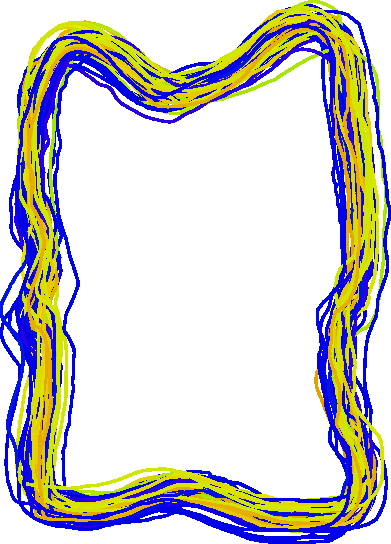
\includegraphics[width=.9\linewidth]{img/registration/unregistered.pdf}
	\end{subfigure}
	\hspace{0.1\textwidth}%
	\begin{subfigure}[b]{0.34\textwidth}
		\centering
		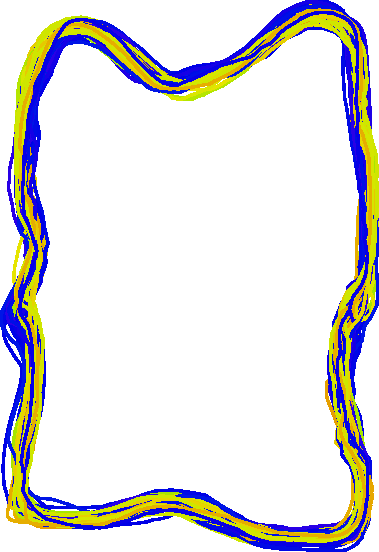
\includegraphics[width=.9\linewidth]{img/registration/registered.pdf}
	\end{subfigure}
	\caption{The bone outlines before (left) and after registration (right)}
	\label{fig:registration}
\end{figure}

Figure \ref{fig:registration} shows the bone outlines before and after the registration step. The differences between the two classes of bones, displayed as yellow and blue here, become more apparent.

\subsection{Correspondence Estimation}

Corresponding points are defined as pairs of semantically identical points in both point sets. Based on these
pairs, the transformation estimation is done.

\subsubsection{Landmarks}

When estimating the correspondence using landmarks, the landmark points are located as described in Section
\ref{sub:landmarks}. Since the number of landmarks is always the same in both outlines, we used the result
as one-to-one correspondences for the registration. We implemented both the angle-based as well as the
space-partitioning-based approaches of the automated landmark extraction. Additionally, we added a method
that evaluates the manually set landmarks of the bones.

\subsubsection{Spline Points}

Another approach to find correspondences was to parameterize the bone outline using a spline and then using $n$
evaluated points on the spline as a normalized representation of the shape. The spline representation consists
of two functions $s_x$, $s_y$ for the $x$ and $y$ coordinates of the outline. We evaluated this spline using $n$
equally spaced parameters $T$ as seen in Equation \ref{eq:registration-spline}.

\begin{equation}
\label{eq:registration-spline}
\begin{split}
& \vec{s}(t) = ( s_x(t), s_y(t) ) \text{ with } 0 \leq t \leq 1 \\
& T = \{ t_i=\frac{i}{n} | i=0, 1, \dots, (n-1) \} \\
& X = \{ \vec{s}(t_i) | t_i \in T \}
\end{split}
\end{equation}

These spline points can be evaluated for all bones in the bone set and provide a one-to-one estimation of correspondences.

\subsubsection{Nearest Neighbors}

All previously suggested approaches have one distinct disadvantage: The correspondences are static, meaning they don't
change after an iteration (although the positions of the automatically found landmarks might change). To compensate this
we implemented a nearest-neighbor approach to estimate correspondences. The resulting algorithm is very similar to
\cite{besl1992method} but uses other transformation estimators.

To find the correspondences for $X$ in $Y$ we simply use the nearest neighbor $NN_Y(\vec{x}_i)$ for each point $\vec{x}_i$ in $X$.

\begin{equation}
NN_Y(\vec{x}_i) = \arg\min_{y_i \in Y}(dist(\vec{x}_i, \vec{y}_i))
\end{equation}

The correspondences found with this method might change after each iteration. This is beneficial for already registered
outlines.

\subsection{Transformation Estimation}

The transformation estimation is done for the selected corresponding points only and then applied to all points in
the point set.

\begin{figure}[h]
	\centering
	\begin{subfigure}[b]{0.24\textwidth}
		\centering
		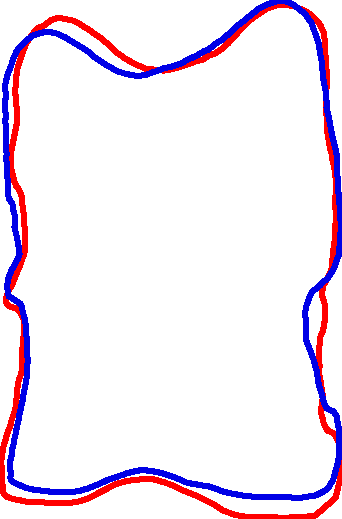
\includegraphics[width=.85\linewidth]{img/registration/single-before.pdf}
		\subcaption{unregistered}
	\end{subfigure}
	\begin{subfigure}[b]{0.24\textwidth}
		\centering
		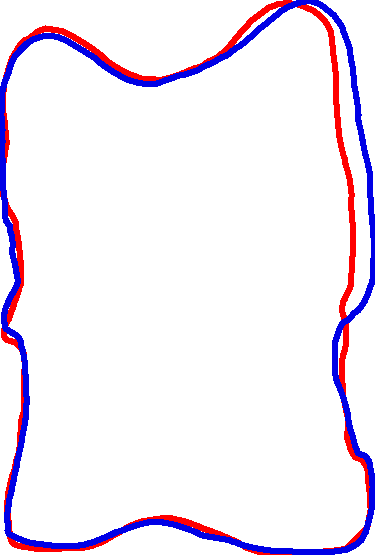
\includegraphics[width=.85\linewidth]{img/registration/single-procrustes.pdf}
		\subcaption{Procrustes}
	\end{subfigure}
	\begin{subfigure}[b]{0.24\textwidth}
		\centering
		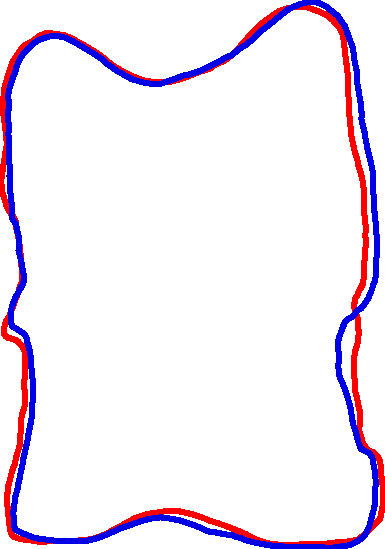
\includegraphics[width=.9\linewidth]{img/registration/single-affine.pdf}
		\subcaption{affine}
	\end{subfigure}
	\begin{subfigure}[b]{0.24\textwidth}
		\centering
		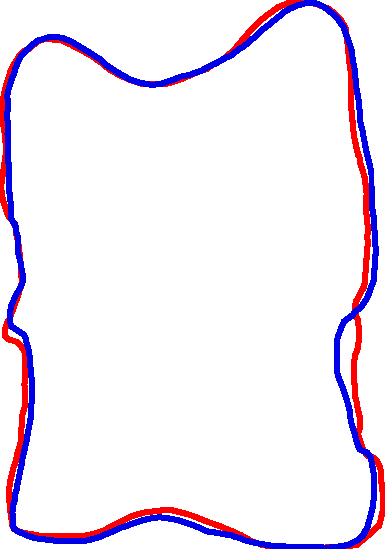
\includegraphics[width=.9\linewidth]{img/registration/single-projective.pdf}
		\subcaption{projective}
	\end{subfigure}
	\caption{A single registration step using same correspondences but different transformation estimations}
	\label{fig:slic}
\end{figure}

\subsubsection{Procrustes Transformation}
\label{subsub:procrustes}

Procrustes transformation is a transformation that uses a combination of translation, scaling and rotation. This kind of
transformation preserves the original shape of the object, making it a similarity transformation. In our case reflection
was not necessary since all the objects were previously aligned already. The Procrustes transformation is closely related to the
Procrustes analysis. To superimpose a point set $X$ onto a reference point set $Y$ three steps are necessary. The first
two steps (transformation into center and uniform scaling) were already done in the normalization step. The only
estimation necessary is the one of the angle $\theta$ which the point set $X$ needs to be rotated by to get the registered
point set $R$.

\begin{equation}
\begin{split}
& \theta = \arctan{\left( \frac{\sum\limits_{i = 1}^n(x_{ix}y_{iy} - x_{iy} y_{ix})}{\sum\limits_{i = 1}^n (x_{ix} y_{ix} + x_{iy} y_{iy}) } \right)} \\
& \vec{r_i} = { (x_{ix} \cos\theta - x_{iy} \sin\theta, x_{ix} \sin\theta - x_{iy} \cos\theta) } \\
& R = \{ \vec{r_1}, \cdots, \vec{r_n} \}
\end{split}
\end{equation}

When executing the Procrustes transformation in an iterative manner using differing correspondence estimations,
translation and scaling need to be re-estimated as well.

\subsubsection{Affine Transformation}
\label{subsub:affine}

An affine transformation is a transformation between two spaces that preserves three properties:

\begin{itemize}
\item Collinearity: All points on a line still lie on a line after the transformation
\item Parallelism: Two parallel lines are still parallel after the transformation
\item Proportions of distances: Three points on a line have the same ratio of distances after the transformation
\end{itemize}

Estimating kind of transformation allows for more flexibility to align the shapes. At the same time it has the
disadvantage of actually changing the shape of the object. The Procrustes transform we presented in Section
\ref{subsub:procrustes} is a subset of the affine transformation. Other transformations include shearing and combination of all presented transformations. Since the bones were sometimes photographed from
slightly different perspectives, we allowed the slight change in shape in this case, especially because was
applied to the whole object.

An affine transformation is represented by a $3\times3$ transformation matrix $\mathbf{A}$. We can write a transform that
superimposes a point set $X$ onto a point set $Y$ in homogeneous coordinates as:

\begin{equation}
\label{eq:projectivetransformation}
\begin{split}
& \vec{r_i} = \mathbf{A} \vec{x_i} \\
& R = \{ \vec{r_i}, \cdots, \vec{r_n} \}
\end{split}
\end{equation}

The estimation of the affine transform was done using the scikit-image python library \cite{van2014scikit}.
It uses a linear equation system to solve for $A$ minimizing the mean squared error between $R$ and $Y$.

\subsubsection{Projective Transformation}

A projective transformation, often referred to as homography is another kind of transform we implemented.
Projective transformations are all transformations that adhere to the collinearity constraint introduced
in Section \ref{subsub:affine}. Since projective transformations are transformations specifically used
to study perspective, we used it to correct for differing perspectives of the bone photographies.

A projective transformation can be represented similarly to an affine transform as defined in Equation
\ref{eq:projectivetransformation}. The estimation was done by scikit-learn \cite{van2014scikit} as well. 

\section{Shape Comparison}
\label{sec:shape-comparison}

After registering the bone shapes, we could test them for significant local shape variations. To compare the shapes, we evaluated windows around $n$ points, each defined by an angle $\rho_i$. An evaluation
point therefore represents a neighborhood around itself. For each of these neighborhoods
we calculated a set of features for each bone in the database. Then a support vector machine
was used to determine the separability of the established classes at these points. Based on 
these separability measures, we can then decide whether the two classes can be distinguished
at this point or not. 

\subsection{Selection of Evaluation Windows}

To determine separabilities we need to sweep the outlines of the bone at $n$ angles $\rho_i$. At each of these angles we need to cut a window from each of the outlines $B \in DB$. For this purpose we implemented two approaches that cut semantically similar windows at each angle.

\begin{figure}[h]
	\centering
	\begin{subfigure}[b]{0.32\textwidth}
		\centering
		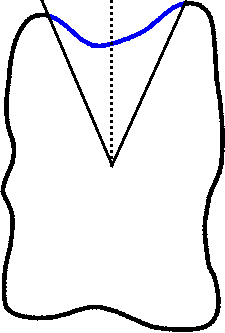
\includegraphics[width=.6\linewidth]{img/window-extraction/by-angle.pdf}
		\subcaption{By angle}
		\label{fig:window-extraction-angle}
	\end{subfigure}
	\begin{subfigure}[b]{0.32\textwidth}
		\centering
		
\includegraphics[width=.6\linewidth]{img/window-extraction/by-length.pdf}
		\subcaption{By length}
		\label{fig:window-extraction-length}
	\end{subfigure}
	\begin{subfigure}[b]{0.32\textwidth}
		\centering
		\raisebox{1cm}{
		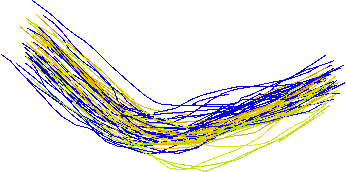
\includegraphics[width=.9\linewidth]{img/window-extraction/windows.pdf}
		}
		\subcaption{Extracted windows}
		\label{fig:window-extraction-all}
	\end{subfigure}
	\caption{Window extraction at $\rho=90^\circ$}
	\label{fig:window-extraction}
\end{figure}


\subsubsection{By Angle}
\label{subsub:windowbyangle}

The first approach to select an evaluation window by cutting a section of a certain angular
width from the bone outline. The window in this method is defined by $\rho$ and $\Delta\rho$
and is derived by ray casting from the coordinate center at the angles $\rho - \Delta\rho$ and 
$\rho + \Delta\rho$ and using the polygon segment that lies in between these intersection points. 

To find an intersection point at a certain angle $\rho$, the spline $\vec{s_B}(t) = (s_{Bx}(t), s_{By}(t))$ was evaluated at $k=250$ evenly spaced
parameters $t_i \in [0,1]$ for each bone $B \in DB$. This evaluation was joined to a polygon
with $k$ line segments $s_i$. The intersection $\vec{i_B}(\rho)$ between this polygon and the ray was calculated and
the line segment $s_i$ that had this intersection on it was selected. $s_i$ is the line
segment between $\vec{s_B}(t_i)$ and $\vec{s_B}(t_{i+1})$ or $\vec{s_B}(0)$ for $i=k$.

To extract the exact parameter $t_{int}(\rho)$ where the intersection occurred, The distances
between the intersection $\vec{i_B}(\rho)$ and the endpoints of the line segment $s_i$ were put into relation.

\begin{equation}
t_{int}(\rho) =
\frac{|\vec{i_B}(\rho) - \vec{s_B}(t_{i+1})|}{|\vec{s_B}(t_i) - \vec{s_B}(t_{i+1})|} t_i +
\frac{|\vec{i_B}(\rho) - \vec{s_B}(t_i)|}{|\vec{s_B}(t_i) - \vec{s_B}(t_{i+1})|} t_{i+1}
\end{equation}

This leads to a good estimation of $t_{int}$ and the intersection point $\vec{s_B}(t_{int})$
for each bone $B$ at the angle $\rho$.

Performing this calculation for $\rho-\Delta\rho$ and $\rho+\Delta\rho$ leads to two spline
parameters $t_{\rho-\Delta\rho}$ and $t_{\rho+\Delta\rho}$ in between the spline can be 
evaluated to get the evaluation window.

The drawback of this method is that bones that are not aligned very well get shorter windows
if their outline lies closer to the coordinate center and longer windows otherwise. The same mechanism leads to differing window lengths overall, because the bone is rectangular. This 
might lead to unwanted results when doing the comparison since the considered windows are
not semantically equal. 

\subsubsection{By Length}
\label{subsub:windowbylength}

To counteract this mechanism, we implemented another method to extract the evaluation window.
In this approach, a window of a certain length $l$ around a point of evaluation that is defined by the angle $\rho$ is extracted. To find these points we employed ray-casting
as introduced in Section \ref{subsub:windowbyangle}. This leads to a spline parameter
$t_\rho$ which now defines the center of our window.

To get a window from $t_\rho$, we expand the initial window $[t_{rho}-\Delta t_i,
t_{rho}+\Delta t_i]$ with $\Delta t_0 = 0$ and $i=0$ iteratively. With each iteration we add a constant value $\delta$ to $\Delta t_i$.

\begin{equation}
\Delta t_i = \Delta t_{i-1} + \delta
\end{equation}

When the window length is equal, or exceeds the required length $l$, we abort and get the current
window as the result of our calculation.

\begin{equation}
\int_{t_\rho - \Delta t_i}^{t_\rho + \Delta t_i} ||\vec{s_B}(t)|| dt \leq l
\end{equation}

Similarly to the angle based method presented in Section \ref{subsub:windowbyangle}, this leads to the spline parameters $[t_{rho}-\Delta t_i, t_{rho}+\Delta t_i]$ of the last iteration $i$, in between which the window at angle $\rho$ of length $l$ is defined.

The windows extracted by this method have approximately (because of the discrete
characteristic of the algorithm) the same length, making them more similar across
the different bones.

\subsection{Feature Extraction}
\label{sub:featureextraction}

To compare the two classes at an angle $\rho$, we needed to extract features from the
window defined by $[t_{start}, t_{end}]$ for each bone. We evaluated several feature
extraction methods for this purpose. Most of these methods operate on a set of points
$S$ that are created by evaluating the spline at $k$ equally spaced parameters. We call $k$ the number of evaluations per window.

\begin{equation}
\begin{split}
& T = \{ t_i=t_{start} + \frac{i}{n} * (t_{end}-t_{start}) | i=0, 1, \dots, (k-1) \} \\
& S = \{ \vec{s}(t_i) | t_i \in T \}
\end{split}
\end{equation}  

\subsubsection{Flattened Points}
\label{subsub:features-flattened}

The simplest feature vector we used is to use a flattened version of $S$ as the feature
vector. We consider this the baseline of our algorithm.

\begin{equation}
\vec{f} = \left( \begin{array}{c}
s_x(t_0) \\
s_y(t_0) \\
\vdots \\
s_x(t_{k-1}) \\
s_y(t_{k-1})
\end{array} \right)
\end{equation}

\subsubsection{Distance to Center}

Another feature based on the point set $S$ is the distance of each point $s(t_i)$ to the
center. This feature was considered	to be more robust because it offers a lower dimensionality
than to simply flatten the points.

\begin{equation}
\vec{f} = \left( \begin{array}{c}
||s(t_0)|| \\
\vdots \\
||s(t_{k-1})||
\end{array} \right)
\end{equation}

\subsubsection{Distance to Center and Curvature}
\label{subsub:featuredistancetocenterandcurvature}

To additionally take the relationships in between the points into account we considered
to take the curvature of the spline evaluation into account as well. The curvature $\kappa$ of the spline at the parameter $t_i$ can be calculated as following.

\begin{equation}
\kappa(t_i) = \frac{|s_x^\prime(t_i) s_y^{\prime\prime}(t_i) - s_y^\prime(t_i) s_x^{\prime\prime}(t_i)|}{(s_x^\prime(t_i)^2 + s_y^{\prime}(t_i)^2)^{3/2}}
\end{equation}

The feature vector then consists of a combination of distances and the curvature of the
corresponding points.

\begin{equation}
\vec{f} = \left( \begin{array}{c}
||s(t_0)|| \\
\kappa(t_0) \\
\vdots \\
||s(t_{k-1})|| \\
\kappa(t_{k-1})
\end{array} \right)
\end{equation}

\subsubsection{Curvature of Distance to Center}

For this feature the idea was to only use the relationship between the points in $S$ and describe
the polygon section by the curvature $\kappa$ of the distances to the center. Since the distance 
to the center is no longer a parameterized curve the equation for $\kappa$ differs from
Section \ref{subsub:featuredistancetocenterandcurvature}.

\begin{equation}
\begin{split}
& d(t_i) = ||s(t)_i|| \\
& \kappa(t_i) = \frac{|d^{\prime\prime}(t_i)|}{(1 + d^\prime(t_i)^2)^{2/3}}
\end{split}
\end{equation}

The feature vector is then composed of the curvature of the points in the point set $S$.

\begin{equation}
\vec{f} = \left( \begin{array}{c}
\kappa(t_0) \\
\vdots \\
\kappa(t_{k-1})
\end{array} \right)
\end{equation}

\subsubsection{Derivation from Mean Bone}

The concept of this feature was to use the fact that the mean bone outline is derived from both classes.
Differences in the shape of the two classes should show in derivations from the mean bone outline that
occur in different directions. For this purpose we need to calculate the mean bone $\bar{B} = \{ (\bar{b}_{x0}, \bar{b}_{y0}), \cdots, (\bar{b}_{xk-1}, \bar{b}_{yk-1}) \}$ for the current window of all bones $B \in DB$ first. $(s_{xB}(t), s_{yB}(t))$ defines the spline representation and $T_B = \{ t_{B0}, \cdots t_{Bk-1} \}$ is the extracted window for each bone $B$. The feature vector is then defined by the difference between the mean bone and
each evaluation of the spline.

\begin{equation}
\begin{split}
& \bar{b}_{xi} = \frac{1}{|DB|} \sum_{B \in DB} s_{xB}(t_{Bi}) \\
& \bar{b}_{yi} = \frac{1}{|DB|} \sum_{B \in DB} s_{yB}(t_{Bi}) \\
& \vec{f}_B = \left( \begin{array}{c}
s_{xB}(t_{B0}) - \bar{s}_{x0} \\
s_{yB}(t_{B0}) - \bar{s}_{y0} \\
\vdots \\
s_{xB}(t_{Bk-1}) - \bar{s}_{xk-1} \\
s_{yB}(t_{Bk-1}) - \bar{s}_{yk-1} \\
\end{array} \right)  
\end{split}
\end{equation}

\subsubsection{Spline Derivatives}

Spline derivatives can be used to analyze the shape of an object as well. Changes in the shape reflect heavily
on the derivatives since they show the direction the outline is currently bending to. To filter out high frequency
changes which occur due to the uneven surface of the bone, smoothing is applied to the spline. The smoothing acts as a low-pass filter in frequency space. We can then build the feature vector from the spine derivatives.

\begin{equation}
\vec{f}_B = \left( \begin{array}{c}
s^\prime_{x}(t_{0}) \\
s^\prime_{y}(t_{0}) \\
\vdots \\
s^\prime_{x}(t_{k-1}) \\
s^\prime_{y}(t_{k-1}) \\
\end{array} \right)  
\end{equation}

\subsection{Dimensionality Reduction}

Depending on the number of evaluations $k$ in the feature extraction step, shown in Section
\ref{sub:featureextraction}, the dimensionality of the feature vector for each bone is relatively high. Most of 
the feature vectors have a dimensionality $d = 2k$ or $d = k$. Depending on the value of $k$, this might become
a feature vector of $> 50$ dimensions.

To further analyze these features, we decided to introduce an optional step where principal component analysis
(PCA) is applied to find the main components of the feature vectors as presented in Section \ref{section:pca}. 

Scikit-learn \cite{pedregosa2011scikit} provides an implementation of PCA, which we used to reduce the number of features to a user-defined number.

\subsection{Calculation of Separability Measures}

After extracting features $f_B$ for each bone $B \in DB$ at a certain evaluation point, the last step in the
algorithm is to calculate an indicator that shows whether the two classes can be separated well around this point.
This indicator can be used to show the location of the characteristic differences on the bone outline. For this
purpose we used a Support Vector Machine to calculate several separability measures.

\subsubsection{Margin}

The SVM has the advantage of having the first separability measure built in: The width of the margin between the
support vectors and the separating hyperplane $D$. Since the soft margin method is used to train the SVM, allowing for incorrectly labeled observations, this is the distance to the nearest cleanly split examples. The margin is 
defined using the normal vector of the separating hyperplane $\vec{w}$. We used all observations $TR = \{ f_B \mid B \in DB \}$ to train the SVM $K$ in this case.

\begin{equation}
m = \frac{2}{||\vec{w}||}
\end{equation}

\subsubsection{Observed Accuracy}

Since the margin might incorporate incorrectly classified examples, we decided to use other separability measures
as well to confirm the results defined by the margin. For this purpose we used the observed accuracy metric of the SVM classifier $K$, trained with all observations as well. The class of the observation is here denoted as $C(\vec{o})$
while the predicted class is denoted as $K(\vec{o})$.

\begin{equation}
a_{TR}(K) = \frac{|\vec{o} \in TR | K(\vec{o}) = C(\vec{o})|}{|TR|}
\end{equation}

\subsubsection{Mean Confidence Score}
\label{subsub:mean-confidence-score}

Using the SVM for classification also allowed us to see how well an observation can be assigned to a class. This
is called a confidence score. The confidence score for the SVM is the distance from the observation to the dividing
hyperplane $D$. We can use this to calculate a mean confidence score for all observations for the current evaluation point.

\begin{equation}
c_{TR}(K) = \frac{1}{|TR|} (\sum_{\vec{o} \in TR \mid K(\vec{o}) = C(\vec{o})} dist(\vec{o}, D) - \sum_{\vec{o} \in TR \mid K(\vec{o}) \neq C(\vec{o})} dist(\vec{o}, D))
\end{equation}

\subsubsection{Mean Cross-Validation Accuracy}
\label{subsub:cross-validation-accuracy}

In classification applications it's usually beneficial to separate the training and test sets to see how well a
classifier can be generalized. Since our application is not a classifier but still very close to it, we wanted
to make sure that the SVM could be generalized as well. When the classifier can be generalized well, the separation
should work as well at this position.

Since our dataset is relatively small, we decided to use cross-validation to verify that the classifier can be
generalized. In cross-validation the dataset is split up into $k$ disjoint sets $S_i$ each of which holds $\frac{|DB|}{k}$ observations. For our case we used $4$ items per set in a stratified manner. Stratified cross-validation is done by using the same ratio of classes inside each disjoint set as inside the whole database. The cross-validation is then
executed by using all but one set as the training data and the remaining one as the test data. This is done $k$ times, so each set is used as test data once.

\begin{equation}
\begin{split}
& TR_i = DB \setminus S_i \\
& TE_i = S_i 
\end{split}
\end{equation}

Using these sets $k$ SVMs $K_i$ are trained. The mean accuracy on the test sets of each classifier is then used
as the measure.

\begin{equation}
\bar{a} = \frac{1}{k} \sum_{i=1}^k \frac{1}{|TE_i|} | \{\vec{o} \in TE_i | K(\vec{o}) = C(\vec{o}) \}| 
\end{equation}

\subsubsection{Mean Cross-Validation Confidence}
\label{subsub:cross-validation-confidence}

The mean cross-validation confidence score is closely tied the the mean confidence score presented in Section \ref{subsub:mean-confidence-score} and the cross validation accuracy presented in the previous section. The selection of training and test data works similarly to the cross-validation accuracy metric. Instead of using the mean accuracy, we are using the distance from the hyperplane of each observation in the test data. This allows us to get a more accurate metric for separability while still using cross-validation to ensure the generalization of our algorithm.

\begin{equation}
\bar{c} = \frac{1}{k} \sum_{i=1}^k c_{TR_i}(K_i)
\end{equation}

\chapter{Detection of Differences That Are Measurable On-Site}
\label{chapter:measurable-differences}

The method presented in Chapter \ref{chapter:detecting-shape-variations} is useful for finding general differences in shape in between two classes of data. But these differences can only be located, but not measured. Since the zoo-archaeologists also needed a method to classify these bones in the field, we implemented another method with the goal of creating a way to classify the bones with only a slide caliper as a tool.

\section{Definition of Measurable Values}

First we needed to define measurable values that could be extracted from the outline of the bone. For this purpose we decided to use the automatically extracted landmarks that we defined in Section \ref{sub:landmarks}. This method provided us with a sets of points that are semantically identical on each bone. Since these points lie on the extrema of the bones shape, finding them manually should be no problem.

These points can be used to calculate simple features that can be used to classify the bone. Since the point can be located on the bone, but not measured in coordinates, we decided to use distances between these points as features. This way only a few distances need to be measured in the field to be able to decide, with a certain probability, to which class the bone belongs. Since the absolute distance between the landmarks is still not meaningful, because the data was normalized and therefore the distance does not translate into a real-world distance, we decided to use ratios of distances as the input data for finding measurable differences.

\begin{figure}[h]
	\centering
	\begin{subfigure}[b]{0.25\textwidth}
		\centering
		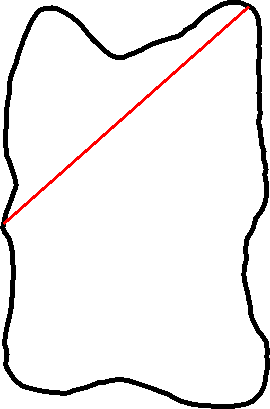
\includegraphics[width=.9\linewidth]{img/measurable/example1.pdf}
	\end{subfigure}
	\begin{subfigure}[b]{0.25\textwidth}
		\centering
		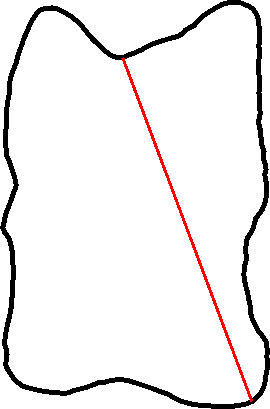
\includegraphics[width=.9\linewidth]{img/measurable/example2.pdf}
	\end{subfigure}
	\begin{subfigure}[b]{0.25\textwidth}
		\centering
		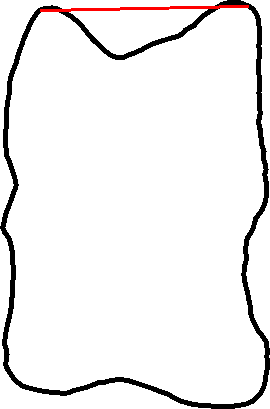
\includegraphics[width=.9\linewidth]{img/measurable/example3.pdf}
	\end{subfigure}
	\caption{Examples for distances between landmarks}
	\label{fig:measurable-distances}
\end{figure}

Both methods to extract landmarks that were presented in Section \ref{sub:landmarks} can be used to extract the landmarks. Depending on the extraction method, some of the distances can be hard to measure. Since the landmarks extracted by space-partitioning lie on extrema in x and y direction, they are preferred when using this method for distances that are parallel to the x- and y-axes. The landmarks extracted by angle are favored for distances that are measured diagonally. This needs to be considered when evaluating the decision tree created by this method.

To create the feature vector for each bone, the initial data is a list of landmarks for this bone $L = \{ \vec{l}_1, ... \vec{l}_n \}$ and a list of landmark combinations $C = \{ (\vec{l}_g, \vec{l}_h), ..., (\vec{l}_i, \vec{l}_j) \}$ with $1 <= g,h,i,j <= n$. The feature vector will then be created from all possible combinations $D$ of the landmark combinations $C$, which correspond to distances between the landmarks.

\begin{equation}
D = C \times C \setminus \{ (C_i, C_i) \mid i = 1 ... k \}
\end{equation}

The distance ratios can then be calculated from this set.

\begin{equation}
\begin{split}
& D = \{ ((\vec{l}_g, \vec{l}_h), (\vec{l}_i, \vec{l}_j)), ..., ((\vec{l}_k, \vec{l}_l), (\vec{l}_m, \vec{l}_n)) \} \\
& \vec{f} = \left( \begin{array}{c}
\frac{||\vec{l}_g - \vec{l}_h||}{||\vec{l}_i - \vec{l}_j||} \\
\vdots \\
\frac{||\vec{l}_k - \vec{l}_l||}{||\vec{l}_m - \vec{l}_n||} \\
\end{array} \right)
\end{split}
\end{equation}

\section{Training a Decision Tree}

To classify the bone we decided to use a decision tree as presented in Section \ref{sec:basics-decision-trees}, because it gives the capability to read the decision path from the classifier. This way the zoo-archaeologist only needs to measure a handful of distances and apply them to the decision tree to figure out the class of the object.

The depth of the decision tree $T$ defines how many distances need to be measured as $m <= depth(T) * 2$. We decided to limit the tree depth to reduce the number of measurements as well as to have a better generalization of the model.

Training the decision tree is pretty straight forward using the feature vectors from the previous section. The split criterion can be selected by the user.

To validate our findings we use the cross-validation method already presented in Section \ref{subsub:cross-validation-accuracy}. We again use stratified sets of 4 items. All but one set are used for training and the remaining one is used as test data. This is done $\frac{|D|}{4}$ times, with each set used once as test data. The mean accuracy of these classifications is used as a metric of how well the decision tree performs.

After having trained the decision tree, the result can be used for manual classification. The split dimensions and values are included in the decision tree. The distances between landmarks represented by the split dimensions need to be measured on the bone that was found in the field. After obtaining the distances the researcher can use a simple calculator to determine the ratios of these distances. The decision tree needs to be applied to these ratios to get the leaf node that corresponds to the found bone. After applying this method correctly the researcher can determine with what probability the bone belongs to a certain class.

\chapter{Experiments}
\label{chapter:experiments}

In this chapter we will show how the algorithm works on both synthetic and real-world data. We ensured that the algorithm works as expected by predefining synthetic classes of data and feeding it into the algorithm. Then we proceeded to use data of real-bone findings to analyze it for distinct shape variations. 

Unless otherwise stated the algorithm was executed using $n=20$ evaluation points per window, a window length of $l=0.2$ and PCA with 4 components. The window extraction is done by length as described in Section \ref{subsub:windowbylength}. We are using the basic flattened spline point feature from Section \ref{subsub:features-flattened} for feature extraction. As the metric we are using the mean cross-validation confidence. Section \ref{sub:comparisonalgorithmparameters} will show how different parameters influence the resulting graph.

\section{Tests on Synthetic Data}

To determine whether the algorithm works as intended, we decided to execute some tests on synthetic data. The reason for that lies in the lack of similar works in this field, so the method needs to be tested thoroughly. Additionally we wanted to see whether the method could be generalized to different forms and how different characteristics of shape influence the result. 

\subsection{Generating Synthetic Data}
\label{sub:generating-synthetic-data}

\begin{figure}[h]
	\centering
	\begin{subfigure}[b]{0.24\textwidth}
		\centering
		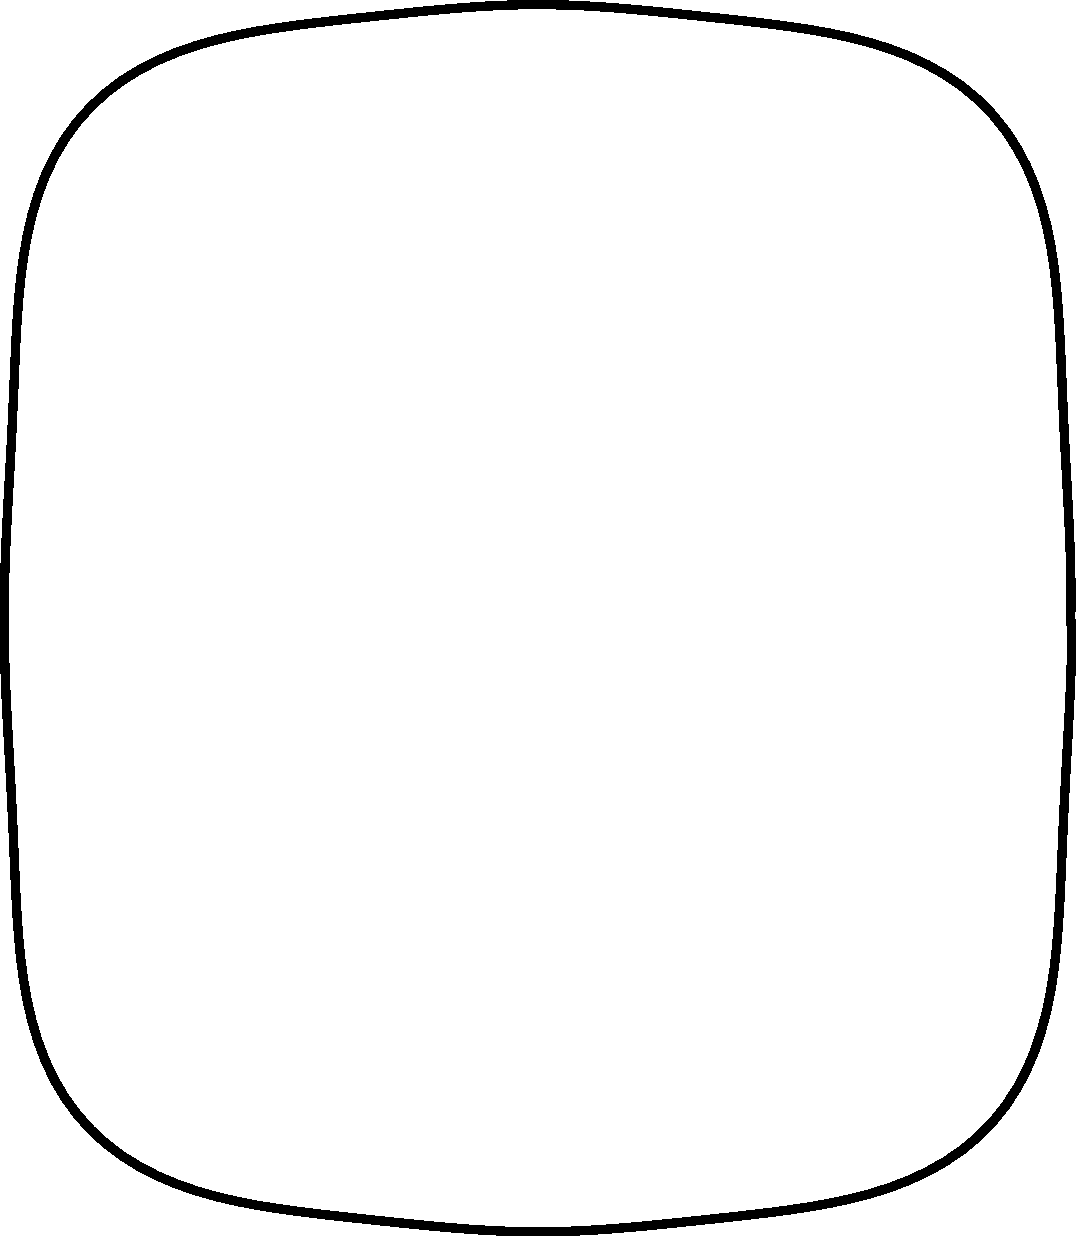
\includegraphics[width=.9\linewidth]{img/synthetic-generation/shapes/1.pdf}
	\end{subfigure}
	\begin{subfigure}[b]{0.24\textwidth}
		\centering
		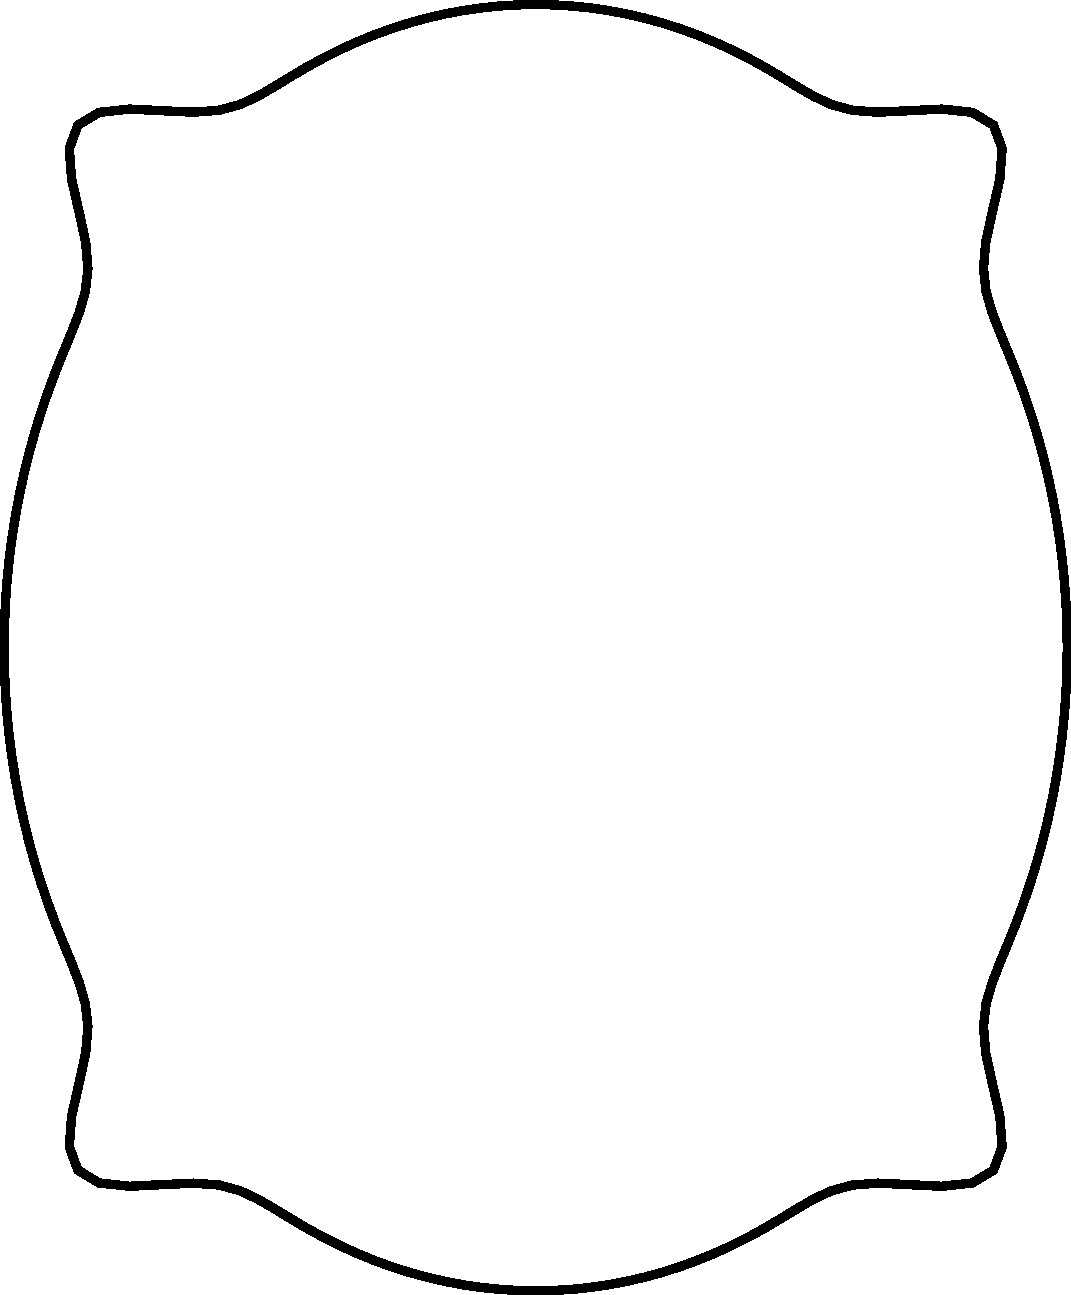
\includegraphics[width=.9\linewidth]{img/synthetic-generation/shapes/2.pdf}
	\end{subfigure}
	\begin{subfigure}[b]{0.24\textwidth}
		\centering
		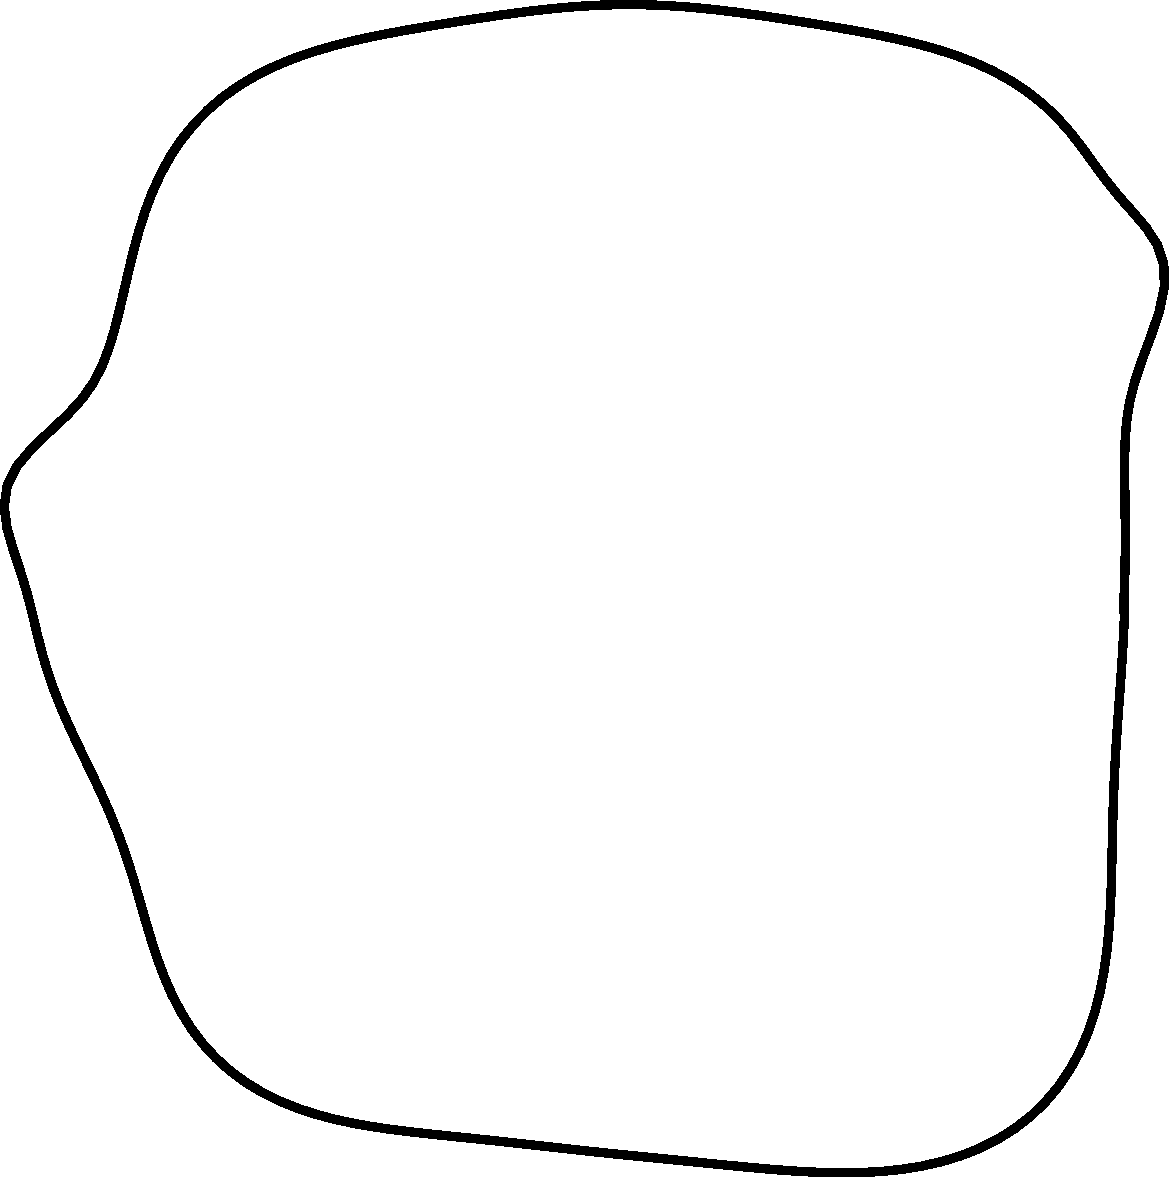
\includegraphics[width=.9\linewidth]{img/synthetic-generation/shapes/3.pdf}
	\end{subfigure}
	\begin{subfigure}[b]{0.24\textwidth}
		\centering
		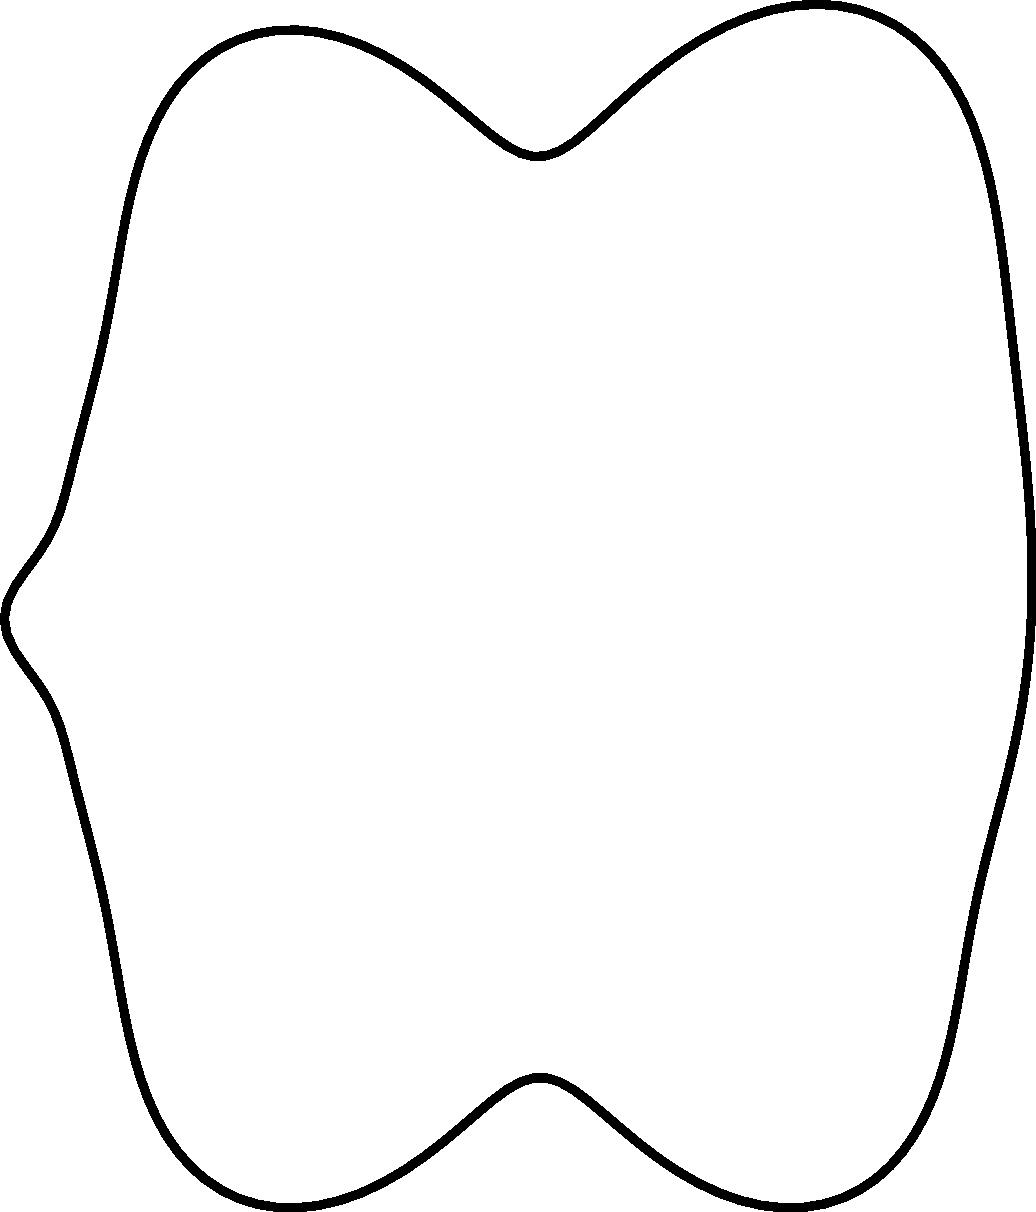
\includegraphics[width=.9\linewidth]{img/synthetic-generation/shapes/4.pdf}
	\end{subfigure}
	\caption{Shapes generated using synthetic generation}
	\label{fig:synthetic-shapes}
\end{figure}

The first step to testing with synthetic data is to define how the data should look like and how this data could be generated. Since the algorithm compares two classes of data we need to create two sets of outlines that have similar characteristics, but also vary inside each set. Additionally because of the style of our algorithm we decided to create circle-shaped test-data. As the base for our data, we use a ellipsoid, which we can vary in eccentricity. Parameterized by angle the ellipsoid can be defined as following, where $\epsilon$ is a parameter that defines the eccentricity of the ellipsoid:

\begin{equation}
	\vec{e}(\alpha) = \left( \begin{array}{c}
		cos(\alpha) \\
		\epsilon sin(\alpha)
	\end{array} \right) 
\end{equation}

To represent shape variations on the bone, we decided to use Gaussian bell curves, which can be stacked onto each other to produce a whole variation of shapes. Each of these bell curves $b_i(\alpha)$ is defined by a height $h_i$, an angle at which the curve has its center $\mu_i$ and a width of the curve $\sigma$. The formula for the curve is applied in the normal direction of the current angle $\vec{n}(\alpha)$, which is defined as:

\begin{equation}
	\vec{n}(\alpha) = \frac{1}{\sqrt{(e_y^\prime(\alpha))^2 + (-e_x^\prime(\alpha))^2}}\left( \begin{array}{c}
		e_y^\prime(\alpha) \\
		-e_x^\prime(\alpha)
	\end{array} \right)
\end{equation}

Using this normal vector the set of bell curves $B$ can be applied to the ellipsoid:

\begin{equation}
	\vec{b}(\alpha) = \sum_{(h_i, \mu_i, \sigma_i) \in B}h_i \vec{n}(\alpha) \exp\left(\frac{-(\mu_i - \alpha)^2}{2 \sigma_i^2} \right )
\end{equation}

The whole shape can be defined by summing these functions together:

\begin{equation}
	\vec{b}(\alpha) = \vec{e}(\alpha) + \vec{b}(\alpha)
\end{equation}

This function needs to be evaluated at $n$ angles $\alpha_i$ with $i = 1 ... n$ to get an outline that can be used as an input for the algorithm.

\begin{equation}
	\alpha_i = \frac{i}{n} 360^{\circ}
\end{equation}

Using this method a variety of shapes can be created, examples for which are shown in Figure \ref{fig:synthetic-shapes}. But they only describe the base shapes for the generation of multiple classes of shapes. From two of these shapes, instances can be created that vary from the base shape to some degree. For that purpose randomized elements are added to the base shape.

\begin{figure}
	\centering
	\begin{subfigure}[b]{0.24\textwidth}
		\centering
		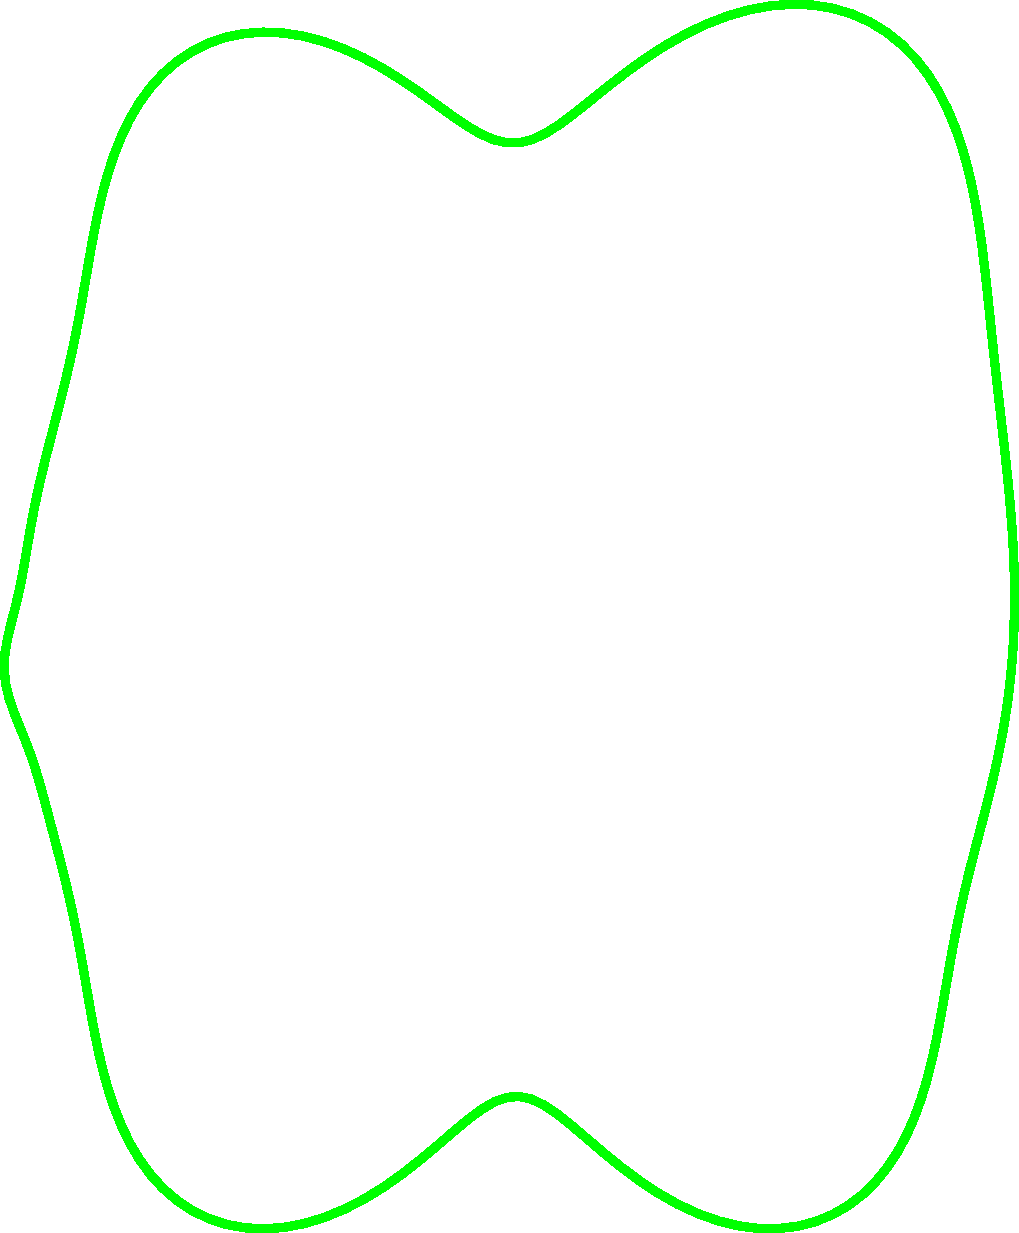
\includegraphics[width=.9\linewidth]{img/synthetic-generation/classes/1-1.pdf}
		\caption{Class A}
		\label{subfig:synthetic-classes:a-1}
	\end{subfigure}
	\begin{subfigure}[b]{0.24\textwidth}
		\centering
		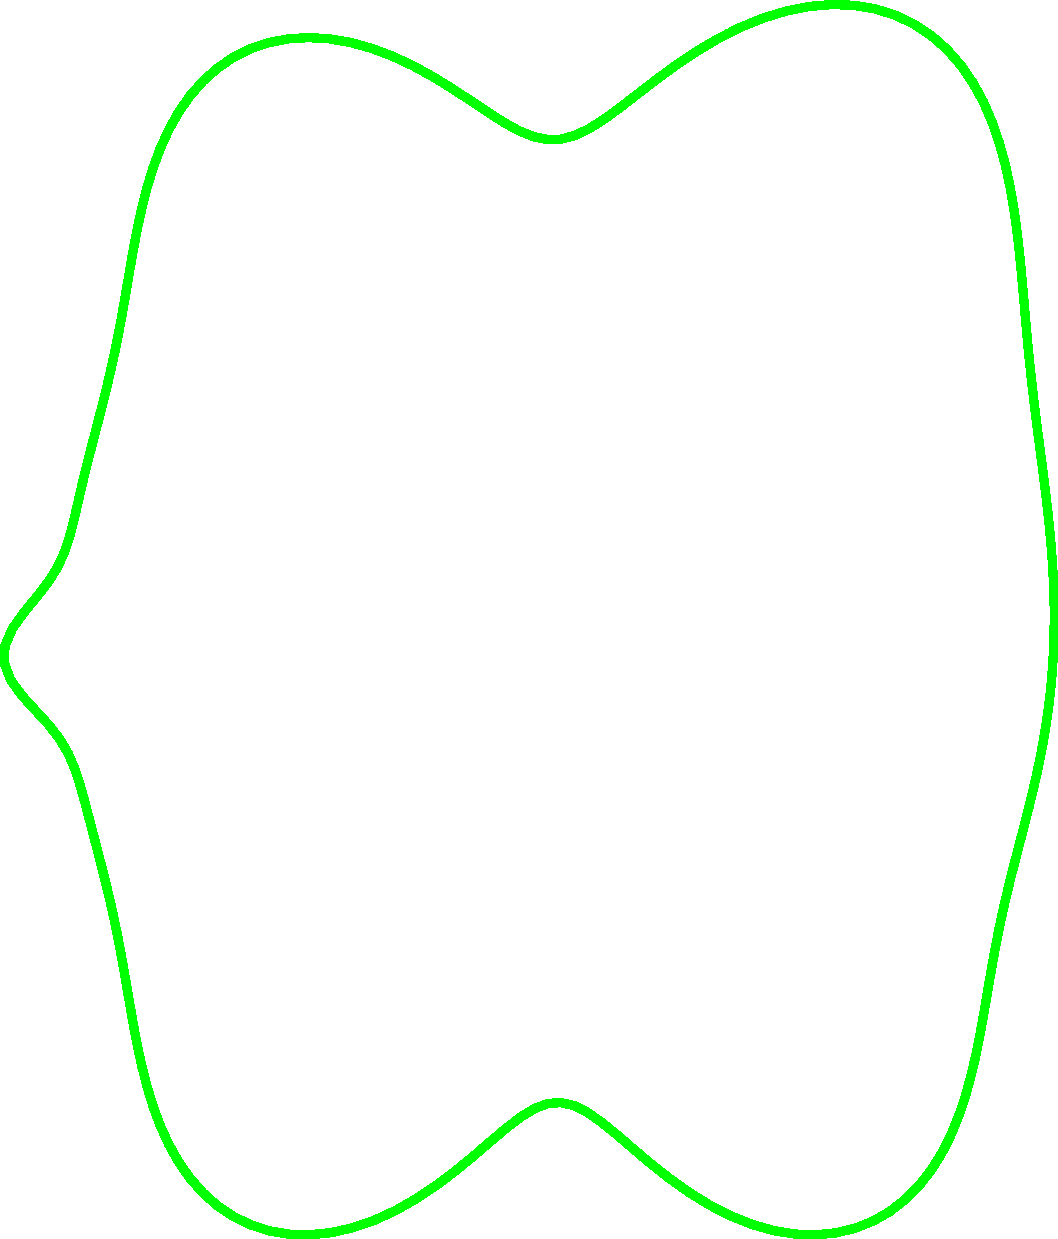
\includegraphics[width=.9\linewidth]{img/synthetic-generation/classes/1-2.pdf}
		\caption{Class A}
		\label{subfig:synthetic-classes:a-2}
	\end{subfigure}
	\begin{subfigure}[b]{0.24\textwidth}
		\centering
		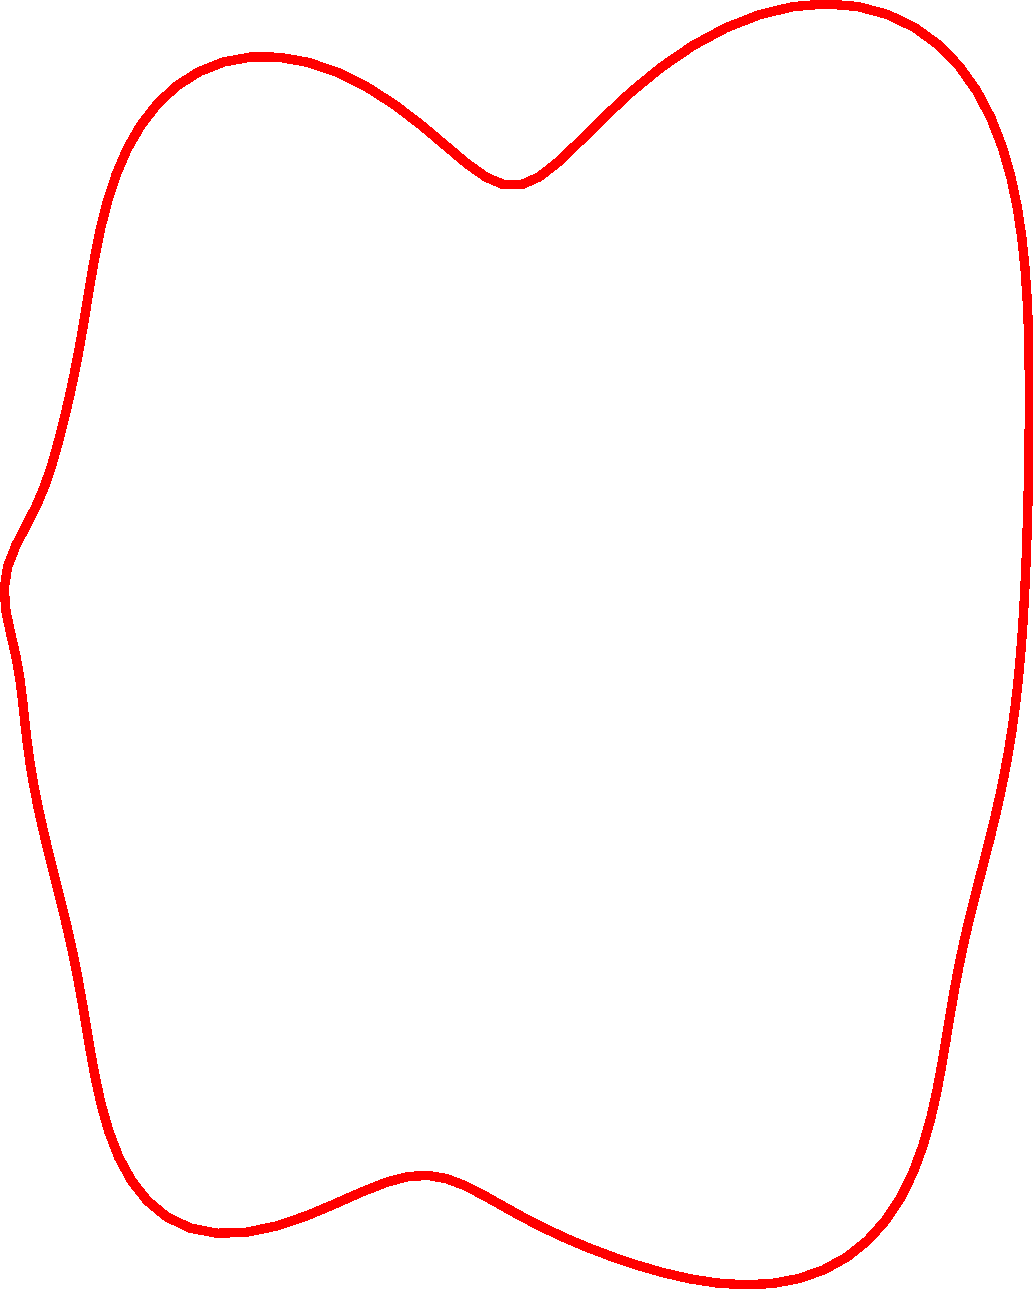
\includegraphics[width=.9\linewidth]{img/synthetic-generation/classes/2-1.pdf}
		\caption{Class B}
		\label{subfig:synthetic-classes:b-1}
	\end{subfigure}
	\begin{subfigure}[b]{0.24\textwidth}
		\centering
		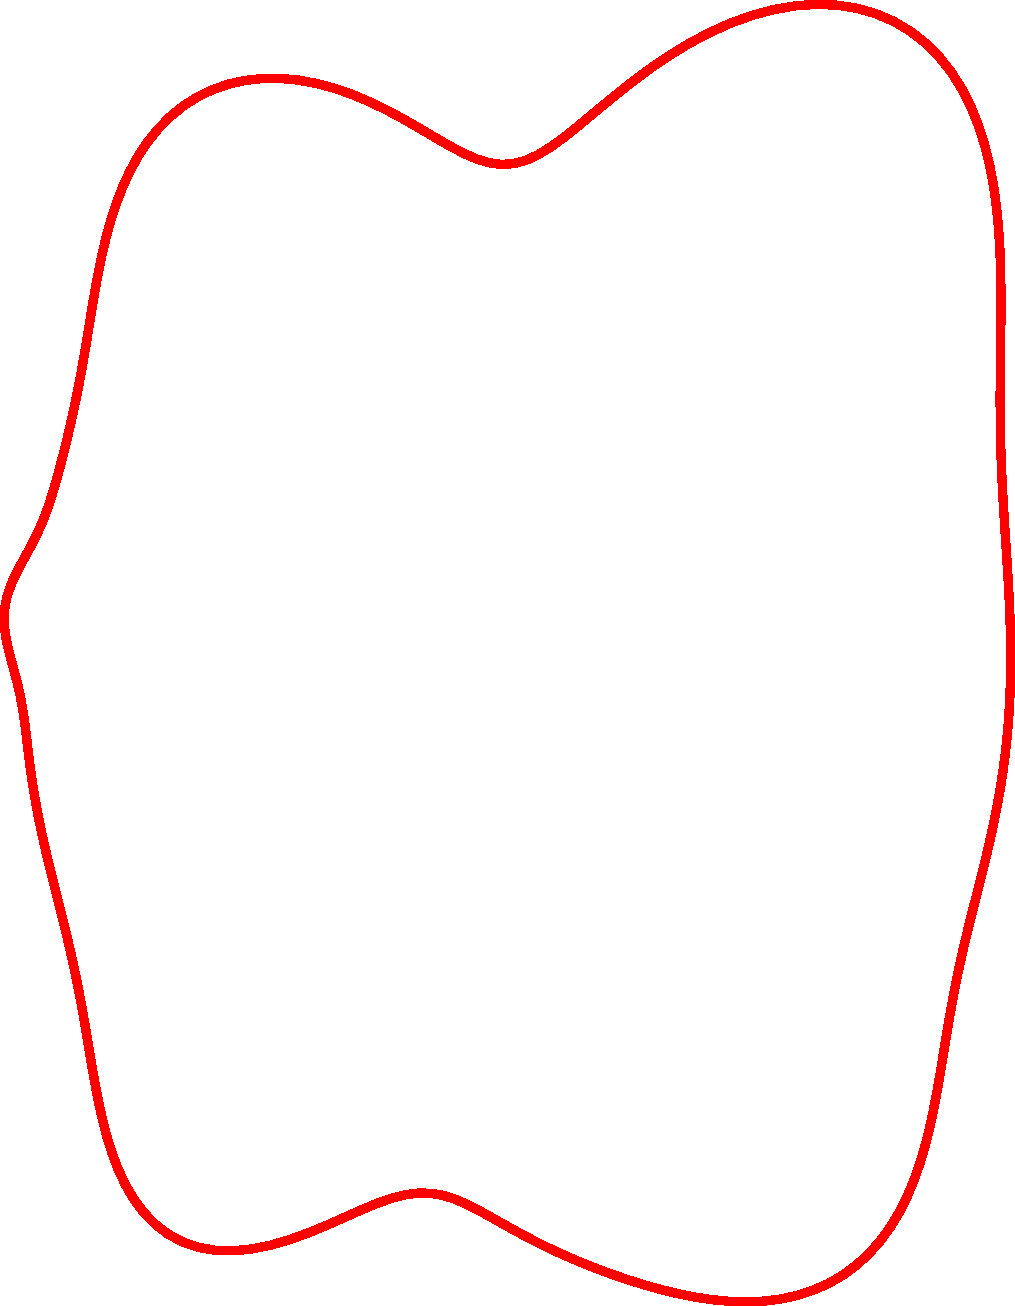
\includegraphics[width=.9\linewidth]{img/synthetic-generation/classes/2-2.pdf}
		\caption{Class B}
		\label{subfig:synthetic-classes:b-2}
	\end{subfigure}
	\caption{Two observations each for two classes of outlines that were synthetically generated}
	\label{fig:synthetic-classes}
\end{figure}


The first randomized elements are class internal randomizations that describe differences in measurement and registration. For each class we can define standard deviations for radius $\sigma_r$, evaluation angles $\sigma_\alpha$ and transformation $\sigma_t$. Randomized values $n_r()$, $n_\alpha()$, $n_t$ based on normal distributions using these parameters are added whenever a value is accessed. The values are adapted as follows:

\begin{equation}
	\begin{split}
		& \vec{t} = \left( \begin{array}{c}
			n_t() \\
			n_t()
		\end{array} \right) \\
		& \vec{e}_r = \begin{pmatrix}
			1 + n_r() & 0 \\
			0 & 1 + n_r() \\
		\end{pmatrix} \vec{e}  + \vec{t} \\
		& \alpha_{ri} = \alpha_i + n_\alpha() \\
	\end{split}
\end{equation}

Additionally the number of evaluation angles $n$ is chosen from a uniform distribution between $n_{min}$ and $n_{max}$.

Similarly to randomizing the overall shapes, the shape variations need to be randomized as well, since the features might occur at slightly different positions in nature. To do this we can add randomized elements to each of the parameters that define a shape variation.

\begin{equation}
	\begin{split}
		& h_{ir} = h_i + n_{hi}() \\
		& \mu_{ir} = \mu_i + n_{\mu i}() \\
		& \sigma_{ir} = \sigma_i + n_{\sigma i}() \\
	\end{split}
\end{equation}

Using this randomization process two classes of semi-randomized data can be built that we can compare using the algorithm presented in Section \ref{sec:shape-comparison}. The classes are already registered, so the comparison is possible without further preprocessing. Since we define the characteristic locations on the bone outline ourselves, we can validate whether they are detected by the algorithm correctly.

Figure \ref{fig:synthetic-classes} shows two classes that were generated using this process. The classes in this figure have their distinct variations in the position of the small left bulge, the location of the indentation at the bottom and the height of the right bulge at the top. It is also noticeable that the small left bulge is different inside of class A, because it is much more distinct in Figure \ref{subfig:synthetic-classes:a-2} than it is in Figure \ref{subfig:synthetic-classes:a-1}. In class B the variation can be seen in the indentation at the top being more shallow in Figure \ref{subfig:synthetic-classes:b-2} than in \ref{subfig:synthetic-classes:b-1} and has slightly shifted to the right.

The generated data is already superimposed so no registration is necessary. To match our real-world data we always created 30 instances of each class for the experiments.

\subsection{Influence of Different Types of Variations in Shape Features}

The first test with randomized data has the goal of visualizing how certain changes in shape in between the classes materialize in the result. Since we cannot determine the type of shape shift from the separability metric itself, we need to know how these shape changes influence the separability metric and how we can determine them using the mean shapes of the classes in combination with the separability metric. For this purpose we determined several characteristic changes in shape that we tested using synthetic data based on the variances from Appendix \ref{appendix:table:synthetic-bone} as the base.

\begin{figure}
	\centering
	\begin{subfigure}[b]{0.45\textwidth}
		\centering
		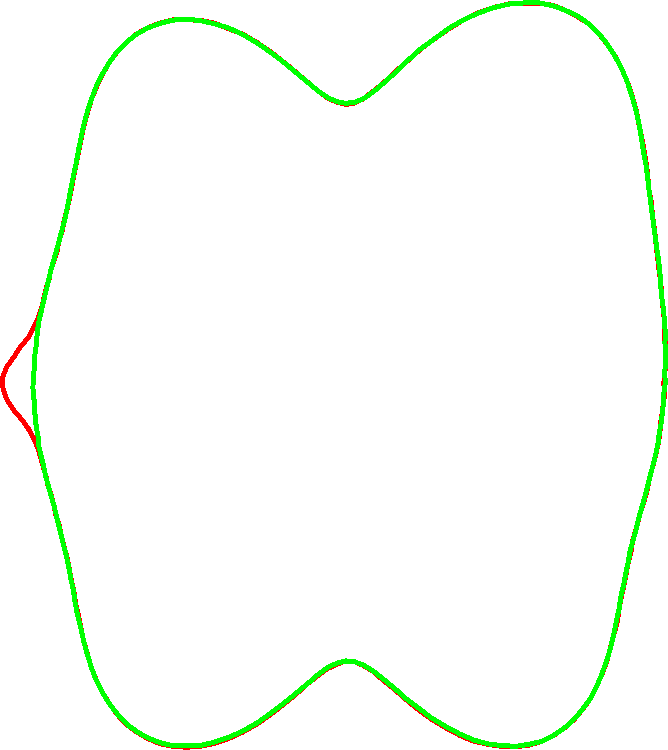
\includegraphics[width=.45\linewidth]{img/results/synthetic/missing-characteristic/missing-characteristic.pdf}
		\subcaption{Missing Feature}
		\label{fig:diff:missing}
	\end{subfigure}
	\begin{subfigure}[b]{0.45\textwidth}
		\centering
		\includegraphics[width=.9\linewidth]{img/results/synthetic/missing-characteristic/0-missing.pdf}
		\subcaption*{}
		\label{}
	\end{subfigure}
	\begin{subfigure}[b]{0.45\textwidth}
		\centering
		\includegraphics[width=.45\linewidth]{img/results/synthetic/shifted/shifter-characteristic.pdf}
		\subcaption{Shifted Feature}
		\label{fig:diff:shifted}
	\end{subfigure}
	\begin{subfigure}[b]{0.45\textwidth}
		\centering
		\includegraphics[width=.9\linewidth]{img/results/synthetic/shifted/0-shifted.pdf}
		\subcaption*{}
		\label{}
	\end{subfigure}
	\caption{Mean input data for two classes (red and green) and separability measure chart for this comparison}
	\label{fig:diff}
\end{figure}

Most features manifest similarly in the separability measure as a very distinctive maximum. An example for this kind of difference can be seen in Figure \ref{fig:diff:missing}. For this comparison we left out a feature at the left side of the bone at an angle of $180^\circ$ as defined in Appendix \ref{appendix:table:synthetic-bone-missing} for one class (green). This is clearly visible as a distinct peak at $180^\circ$ in the respective diagram. The separability measure begins to rise when the window that is cut from the bones includes the missing feature.  

While the differences between the two classes of bones are apparent and even visible to the human eye, the algorithm also detects differences in features that are less dissimilar. The model that is visible in Figure \ref{fig:diff:shifted} was built by moving the feature that creates part of the bottom recess to the left as defined in Appendix \ref{appendix:table:synthetic-bone-shifted}. The difference is still visible in the result, although the absolute value is smaller. Noticeable is also the V-shape of the top of the peak, which can occur if the feature is wider than the window that is cut out of the bone. The separability of the individual parts of the feature are calculated instead of the separability of the full width of the feature. This can be fixed by using a larger window size for the algorithm.

\begin{figure}[h]
	\centering
	\begin{subfigure}[b]{0.45\textwidth}
		\centering
		\includegraphics[width=.45\linewidth]{img/results/synthetic/all/visualization.pdf}
		\subcaption*{}
		\label{fig:diff:all}
	\end{subfigure}
	\begin{subfigure}[b]{0.45\textwidth}
		\centering
		\includegraphics[width=.9\linewidth]{img/results/synthetic/all/0-all.pdf}
		\subcaption*{}
		\label{}
	\end{subfigure}
	\caption{Two classes of data with multiple shape differences}
	\label{fig:all}
\end{figure}

Figure \ref{fig:all} shows two classes of data having multiple differences in shape that are defined in Appendix \ref{appendix:table:synthetic-bone-all}. Additionally to the two previously presented differences, the bump at $45^\circ$ is more distinct as well as the width of indentation at the bottom was increased. The four differences are only visible as 3 in the chart in Figure \ref{fig:all}. This is because two differences affect the bottom crevice. This causes the separability measure to be increased in the absolute value, because the difference between the bones is more distinct. Additionally it looses the V-shape because the separability varies less while only considering parts of the features.

The data presented in Figure \ref{fig:all} is used as the base graph for the following synthetic experiments. While the previous experiments have been executed using only a minimal error component, the next tests will investigate the robustness of the algorithm under the influence of errors.

\subsection{Influence of Variances in Shape Features}
\label{sub:synthetic-variances}

Variances in shape features represent differences in the bone shapes of individual animals. These differences occur because of a different process of growth, changing stress on the bone and even injuries.

We simulate these variances in the bone by adding randomization to the individual bell curves that define the shape of the bone classes. This way each bone gets an individual shape that is increasingly different from each other, but all bones of one class still generate the same mean shape as before. The amount of randomization applied each feature was constant.

\begin{figure}[h]
	\centering
	\begin{subfigure}[b]{0.32\textwidth}
		\centering
		\includegraphics[width=.9\linewidth]{img/results/synthetic/synthetic-errors-feat/0-Features0.pdf}
		\subcaption{\footnotesize$\sigma_{h}=0.01, \sigma_{\mu}, \sigma_{\sigma} = 1.0$}
		\label{fig:results-synthetic-features-0}
	\end{subfigure}
	\begin{subfigure}[b]{0.32\textwidth}
		\centering
		\includegraphics[width=.9\linewidth]{img/results/synthetic/synthetic-errors-feat/1-Features1.pdf}
		\subcaption{\footnotesize$\sigma_{h}=0.025, \sigma_{\mu}, \sigma_{\sigma} = 2.5$}
		\label{fig:results-synthetic-features-1}
	\end{subfigure}
	\begin{subfigure}[b]{0.32\textwidth}
		\centering
		\includegraphics[width=.9\linewidth]{img/results/synthetic/synthetic-errors-feat/2-Features2.pdf}
		\subcaption{\footnotesize$\sigma_{h}=0.05, \sigma_{\mu}, \sigma_{\sigma} = 5.0$}
		\label{fig:results-synthetic-features-2}
	\end{subfigure}
	\caption{Graphs for models with ascending variance in features}
	\label{fig:ascending-variance}
\end{figure}

The result for models with increasingly high variances in shape features can be seen in Figure \ref{fig:ascending-variance}. It is noticeable that all features are still visible, even in the most noisy configuration. The small difference at about $300^\circ$ cannot be encountered from Figure \ref{fig:results-synthetic-features-1} anymore. This happens if a smaller difference in shape is superimposed by the shape variations. The only feature that is not influenced as much is the missing feature at $180^\circ$. This probably happens because it is a distinct variation in shape, not a wider feature that has a similar shape as the other class.

The shape variances presented in this experiment are subjectively larger than those seen in the real-world data. Though we can not rule out that shape variances seen in the real-world are of different character than the ones we presented our algorithm with, it seems to cope well with varying features.

\subsection{Influence of Errors in Shape Measurement}

Errors in shape measurement can have multiple reasons. On the one hand they can result from a bad photograph or a bad image segmentation. On the other hand they can occur when the bone is being chipped or parts of the bone break away over the bone's time in the ground.

These errors are modeled by adding randomization to the evaluation angle and radius of the generation algorithm presented in Section \ref{sub:generating-synthetic-data}. The bone outlines become irregular, but still follow the same mean outline per class.  

\begin{figure}[h]
	\centering
	\begin{subfigure}[b]{0.32\textwidth}
		\centering
		\includegraphics[width=.9\linewidth]{img/results/synthetic/synthetic-errors-radius/0-Radius0.pdf}
		\subcaption{\footnotesize$\sigma_r=0.01, \sigma_\alpha=0.5$}
		\label{}
	\end{subfigure}
	\begin{subfigure}[b]{0.32\textwidth}
		\centering
		\includegraphics[width=.9\linewidth]{img/results/synthetic/synthetic-errors-radius/1-Radius1.pdf}
		\subcaption{\footnotesize$\sigma_r=0.025, \sigma_\alpha=1$}
		\label{}
	\end{subfigure}
	\begin{subfigure}[b]{0.32\textwidth}
		\centering
		\includegraphics[width=.9\linewidth]{img/results/synthetic/synthetic-errors-radius/2-Radius2.pdf}
		\subcaption{\footnotesize$\sigma_r=0.05, \sigma_\alpha=1$}
		\label{fig:ascending-radius-angle-2}
	\end{subfigure}
	\caption{Graphs for models with ascending variance in radius and angle}
	\label{fig:ascending-radius-angle}
\end{figure}

The first noticeable change is the serrated edge of the graph in Figure \ref{fig:ascending-radius-angle}. While the graph still follows the same general outline, the results seem to have more variance when increasing the error. This might occur when certain observations are not classified correctly anymore during validation of the model, because of their distortion. The peaks of the features approximately stay at the same height and become sharper because the less distinct parts of the feature are superimposed by noise.

While a graph like Figure \ref{fig:ascending-radius-angle-2} might not be sufficient to be analyzed for differences in the bone class, we can still see that our method picks up differences in very noisy data. What we have not verified is how bigger broken-off parts of the object influences shape analysis, since our data does not contain such samples.

\subsection{Influence of Errors in Shape Registration}

\begin{figure}[h]
	\centering
	\begin{subfigure}[b]{0.32\textwidth}
		\centering
		\includegraphics[width=.9\linewidth]{img/results/synthetic/synthetic-errors-trans/0-Trans0.pdf}
		\subcaption{\footnotesize$\sigma_t=0.01$}
		\label{fig:ascending-translation-0}
	\end{subfigure}
	\begin{subfigure}[b]{0.32\textwidth}
		\centering
		\includegraphics[width=.9\linewidth]{img/results/synthetic/synthetic-errors-trans/1-Trans1.pdf}
		\subcaption{\footnotesize$\sigma_t=0.025$}
		\label{fig:ascending-translation-1}
	\end{subfigure}
	\begin{subfigure}[b]{0.32\textwidth}
		\centering
		\includegraphics[width=.9\linewidth]{img/results/synthetic/synthetic-errors-trans/2-Trans2.pdf}
		\subcaption{\footnotesize$\sigma_t=0.05$}
		\label{fig:ascending-translation-2}
	\end{subfigure}
	\caption{Graphs for models with ascending variance in translation}
	\label{fig:ascending-translation}
\end{figure}

The last test we executed on synthetic data was how registration errors affect the algorithm. Registration errors are inherent to this method since the shapes cannot be superimposed exactly without any registration error.

We model this registration error as variances in translation in between the shapes. This does not affect the outlines shape, but the position of this outline. Both classes now consist of the same shapes with slightly different positions.

From Figure \ref{fig:ascending-translation} we can see that small or medium registration errors only have little effect on the result of our algorithm. Similarly to the variances of feature from Section \ref{sub:synthetic-variances}, the small feature at $300^\circ$ is lost in the registration error. The missing feature at $180^\circ$ is again the least influenced by the error. While all but this feature fade in Figure \ref{fig:ascending-translation-2}, the registration error encountered in this experiment is larger than the one found in real-word-data.

With this knowledge it might not be necessary to register the bones using a non-similarity transform, avoiding changes in the shape of the bones. While this might lead to smaller separability, we can assure that the data used by the algorithm has not been altered in a possibly biasing fashion.

\section{Tests on Real-World Data}

After validating the algorithm using synthetic data, we advanced by analyzing the shape of real bone findings. The data provided to us is data from domestic and wild sheep classes that are already classified by zoo-archaeologists as explained in Chapter \ref{chapter:problem-definition}. We have a database size of $57$ observations, $29$ of which are in the class of domestic sheep and $28$ of which are wild sheep. We registered the sheep using Procrustes transformation in one iteration with landmarks as correspondences and 20 iterations with nearest neighbors.

\subsection{Results and Compliance with Former Findings} 

\begin{figure}
	\centering
	\begin{subfigure}[b]{0.25\textwidth}
		\centering
		\includegraphics[width=.6\linewidth]{img/results/real/combined_edited.pdf}
		\subcaption{\footnotesize Mean input data}
		\label{fig:main-result-data}
	\end{subfigure}
	\begin{subfigure}[b]{0.35\textwidth}
		\centering
		\includegraphics[width=.9\linewidth]{img/results/real/result_edited.pdf}
		\subcaption{\footnotesize Result}
		\label{fig:main-result-chart}
	\end{subfigure}
	\begin{subfigure}[b]{0.35\textwidth}
		\centering
		\includegraphics[width=.9\linewidth]{img/results/real/distances.pdf}
		\subcaption{\footnotesize Distance of mean bones}
		\label{fig:main-result-distance}
	\end{subfigure}
	\caption{Algorithm applied to domestic (yellow) and wild sheep (blue)}
	\label{fig:main-result}
\end{figure}

The results of the algorithm applied on real-world data can be seen in Figure \ref{fig:main-result-chart}. Figure \ref{fig:main-result-data} shows the mean outlines for domestic (blue) and wild (yellow) sheep and the angles corresponding to the peaks in Figure \ref{fig:main-result-chart}. For reference we plotted the distance between the mean bones in Figure \ref{fig:main-result-distance}.

When comparing the charts of the distance between mean bones and our result it becomes clear that while some of the peaks are visible as well in Figure \ref{fig:main-result-distance}, the peaks are much more distinct using our method. Since we are not only using distances, but essentially the margin between the classes of the bones, our algorithm considers the separability at each angle as well. So if the mean bones diverge, they might do so with such a variance inside at least one class that makes the distance between the mean bones less meaningful. Our method also covers features that vary in position, so they do not express themselves as distinct in the mean bone.

But from the mean bones it is apparent that the highest peak in the result chart corresponds to the parts of the bone where the mean bones diverge the most. It needs to be noted that the maximum separability metric of the result is smaller than that of the synthetic tests, but that is to be expected with real-world data as a combination of measurement errors, variance in shape features and registration errors applies. Nevertheless distinct peaks are visible in the result graph. While the upper half of the bone is highly separable, the lower half is similar in both classes. This agrees with the results of the zoo-archaeologist who also found significant differences in the area between the lateral and medial crest. Our algorithm shows three distinct points in the upper area of the outline which we marked as one, two and three. In the area between these points, the separability decreases, but does not reach zero. Additionally to the points between the crests, our result shows a highly separable area around the out most point on the medial apex.

The first separable point is located in the area around the highest point on the lateral crest marked as one in Figure \ref{fig:main-result}. This difference is not as distinct as the others. It is located right at an intersection between the two mean bones which indicates that it stems from the accumulation of two minor separabilities to the left and right of the evaluation point. The bones of the wild sheep are a bit wider to the right and less high to the left than those of the domestic sheep at this angle. After this key point, the separability falls again, but not to the point of not being separable.

The second separable point is at the angle of $80^\circ$ and marked as two in Figure \ref{fig:main-result}. It is caused by a distinct bulge that is present in most of the Tali of wild sheep. While the bulge is not visible as such in the mean bone, because of variations in position and height, it is noticeable that the mean bone of wild sheep is flatter that the one of domestic sheep around this position. The theory of the zoo-archaeologists is that this bump stems from the different stress level that is put on the bone when the wild sheep stand in mountainous terrain. Domestic sheep usually stand in flat areas so this bulge is not present in their bones.

The third an most significant difference manifests at about $120^\circ$, which corresponds to the medial crest. The medial crest is much more distinctive in domestic sheep than in wild sheep. This is clearly visible in the mean bones of the two classes. Combined with key point two, where the lateral crest is more distinctive as well, it can also be viewed as the depression between the crests being deeper than in wild sheep. According to the experts, this might be caused by the domestic sheep not moving as much inside their pastures as the wild sheep and thus experiencing more stress between the crests.

The last key point lies at about $190^\circ$ at the medial apex. While the other key points all lie in the area that has been examined by the researchers from the zoo-archeology department, this key point has not been analyzed by them. Based on the mean bones, two differences establish themselves at this point. In wild sheep the medial apex is more pronounced as well as shifted lower, towards the out most point of the medial outer edge. 

Apart from the key points the separability graph oscillates around a separability of zero. There exist other minor maxima in the graph, but they are too narrow to represent a separable area. Since the sliding window always incorporates the area around the evaluation angle, they need to be at least as wide as the sliding window.



\subsection{Comparison of Algorithm Parameters}
\label{sub:comparisonalgorithmparameters}

In this section we examine whether changing algorithm parameters manifest as it would be expected in the result. For this purpose we execute the algorithm with the specified parameters on real-world data, while modifying one of the parameters and observe the changes in the result graph.

\subsubsection{Number of Evaluation Points}

\begin{figure}[h]
	\centering
	\begin{subfigure}[b]{0.32\textwidth}
		\centering
		\includegraphics[width=.9\linewidth]{img/results/parameter_comparison/number_of_evaluations/1-10.pdf}
		\subcaption{\footnotesize$n=10$}
		\label{fig:number-evaluations-0}
	\end{subfigure}
	\begin{subfigure}[b]{0.32\textwidth}
		\centering
		\includegraphics[width=.9\linewidth]{img/results/parameter_comparison/number_of_evaluations/4-25.pdf}
		\subcaption{\footnotesize$n=25$}
		\label{fig:number-evaluations-1}
	\end{subfigure}
	\begin{subfigure}[b]{0.32\textwidth}
		\centering
		\includegraphics[width=.9\linewidth]{img/results/parameter_comparison/number_of_evaluations/5-50.pdf}
		\subcaption{\footnotesize$n=50$}
		\label{fig:number-evaluations-2}
	\end{subfigure}
	\caption{Graphs for different parameters for the number of evaluation points in each window}
	\label{fig:number-evaluations}
\end{figure}

In this experiment we will modify the number of points that are evaluated inside each window that is cut from the bone. This relates to increasing the resolution of the algorithm inside each window.

When modifying the number of evaluation points, we would expect the resulting graph to approximately stay constant over different values, since the only difference that is apparent is that finer structures can be represented.

From Figure \ref{fig:number-evaluations}, we can see that the trend of the graph stays the same when increasing the number of evaluations. It becomes also apparent that the absolute separability measure increases when the amount of points is increased. This implies that our separability measure is tied to the dimensionality of the feature vector. This needs to be considered when evaluating different features.

For our experiments we set the number of evaluations to $20$.

\subsubsection{Window Length}

Varying the length of the window that is cut from the bone corresponds to modifying the overall resolution of the algorithm. With a window too small, larger features could be broken up into smaller parts, while with a window too big smaller features that are close by are merged into a single feature.

With a small window size, we expect a very fine grained picture of differences between the bones. When increasing the window size, the graph should be smoothed out and features should slowly merge into larger separable areas.

\begin{figure}[h]
	\centering
	\begin{subfigure}[b]{0.32\textwidth}
		\centering
		\includegraphics[width=.9\linewidth]{img/results/parameter_comparison/window_size/1-0,1.pdf}
		\subcaption{\footnotesize$l=0.1$}
		\label{fig:window-size-0}
	\end{subfigure}
	\begin{subfigure}[b]{0.32\textwidth}
		\centering
		\includegraphics[width=.9\linewidth]{img/results/parameter_comparison/window_size/3-0,4.pdf}
		\subcaption{\footnotesize$l=0.4$}
		\label{fig:window-size-1}
	\end{subfigure}
	\begin{subfigure}[b]{0.32\textwidth}
		\centering
		\includegraphics[width=.9\linewidth]{img/results/parameter_comparison/window_size/4-0,8.pdf}
		\subcaption{\footnotesize$l=0.8$}
		\label{fig:window-size-2}
	\end{subfigure}
	\caption{Graphs for different parameters for window length}
	\label{fig:window-size}
\end{figure}

Figure \ref{fig:window-size} shows separability graphs for multiple window sizes. As we expected, the features get wider and merge into each other when increasing the parameter. Additionally, while small window sizes generate relatively smooth graphs, they become increasingly jagged. This might result from the window size getting larger without the number of evaluations increasing so more information is included in a vector of the same dimensionality. This way the variations between the feature vectors get bigger as well. When two features merge the separability is averaged between them as visible in Figure \ref{fig:window-size-2} with key points one ($60^\circ$) and two ($80^\circ$) or key point four ($190^\circ$). The largest feature is not influenced by this because it's width exceeds the window width, so only the periphery of the feature is merged with others.

We chose a medium window length of $0.2$ to incorporate larger features while not producing a jagged graph.

\subsubsection{Window Extraction Method}

We implemented two algorithms for window extraction: By angle or by length. When extracting the windows by angle, the extracted windows seemed semantically less similar compared to the ones extracted by length. In this section we want to confirm that extracting the windows by length also works quantitatively better.

\begin{figure}[h]
	\centering
	\begin{subfigure}[b]{0.32\textwidth}
		\centering
		\includegraphics[width=.9\linewidth]{img/results/parameter_comparison/window_extraction/0-by-angle.pdf}
		\subcaption{\footnotesize By angle}
		\label{fig:window-extraction-graphs-0}
	\end{subfigure}
	\begin{subfigure}[b]{0.32\textwidth}
		\centering
		\includegraphics[width=.9\linewidth]{img/results/parameter_comparison/window_extraction/1-by-length.pdf}
		\subcaption{\footnotesize By length}
		\label{fig:window-extraction-graphs-1}
	\end{subfigure}
	\caption{Graphs for different window extraction strategy}
	\label{fig:window-extraction-graphs}
\end{figure}

The results for different window extraction methods can be seen in figure \ref{fig:window-extraction-graphs}. From the results it is clearly visible that the separability metric produces much more distinct maxima with the extraction method by length while the general trend of the graph stays the same. This might be cause by the window having different widths at each location and bone, compared to a constant width with the method my length.

To ensure identical window lengths everywhere we decided to use the extraction by length, which is also supported by the more distinct results.

\subsubsection{Principal Component Analysis}

In this section we wanted to determine how principal component analysis influences the results of the algorithm. While the SVM works well in high dimensions, our measure is sensitive to the distance to the hyperplane. The distance is prone to the curse of dimensionality, which states that in larger dimensions, distances between objects become more and more similar.

 \begin{figure}[h]
 	\centering
 	\begin{subfigure}[b]{0.32\textwidth}
 		\centering
 		\includegraphics[width=.9\linewidth]{img/results/parameter_comparison/pca/0-No-PCA.pdf}
 		\subcaption{\footnotesize No PCA}
 		\label{fig:pca-0}
 	\end{subfigure}
 	\begin{subfigure}[b]{0.32\textwidth}
 		\centering
 		\includegraphics[width=.9\linewidth]{img/results/parameter_comparison/pca/1-1-PCA-Component.pdf}
 		\subcaption{\footnotesize 1 component}
 		\label{fig:pca-1}
 	\end{subfigure}
 	\begin{subfigure}[b]{0.32\textwidth}
 		\centering
 		\includegraphics[width=.9\linewidth]{img/results/parameter_comparison/pca/4-4-PCA-Components.pdf}
 		\subcaption{\footnotesize 4 components}
 		\label{fig:pca-2}
 	\end{subfigure}
 	\caption{Graphs for differing PCA configuration}
 	\label{fig:pca}
 \end{figure}

Thus we would expect the algorithm to continue working correctly without using PCA, but producing less distinct results. But a missclassification when calculating the separability metric and each observation being far away from the hyperplane might make their influence more substantial. Using PCA and more components, we expect the result to get finer with each component used from the PCA.
 
While we expected the algorithm to work without PCA, it barely does as it is visible in Figure \ref{fig:pca-0}. Two key points are still visible, but key point two at originally $80^\circ$ has shifted a few degrees to $90^\circ$. The most obvious change is that the previously largest difference in the bones at $119^\circ$ is not detected anymore at all. With other experiments we confirmed that the accuracy is now low at this point, so the outlines seem not to be separable anymore. We tested using other features than the flattened spline points, and determined that when using features with additional information than location, this effect did not occur. When using PCA the separability reappears at each key point, even when only using a single component as shown in Figure \ref{fig:pca-1}. Increasing the number of components eliminates the jumps in the graph, for example at $60^\circ$ or $90^\circ$.

For our purposes we choose PCA with 4 components to ensure separability of the classes and smoothness of the resulting graph.

\subsubsection{Comparison of Features}

\begin{figure}[h]
	\centering
	\begin{subfigure}[b]{0.32\textwidth}
		\centering
		\includegraphics[width=.9\linewidth]{img/results/parameter_comparison/features/0-Flattened-Splines.pdf}
		\subcaption{Flattened splines \\ \phantom{lb}}
		\label{fig:features-0}
	\end{subfigure}
	\begin{subfigure}[b]{0.32\textwidth}
		\centering
		\includegraphics[width=.9\linewidth]{img/results/parameter_comparison/features/1-Distances-To-Center.pdf}
		\subcaption{Distances to center \\ \phantom{lb}}
		\label{fig:features-1}
	\end{subfigure}
	\begin{subfigure}[b]{0.32\textwidth}
		\centering
		\includegraphics[width=.9\linewidth]{img/results/parameter_comparison/features/2-Distances-To-Center-and-Curvature.pdf}
		\subcaption{Distances to center and curvature}
		\label{fig:features-2}
	\end{subfigure}
	\begin{subfigure}[b]{0.32\textwidth}
		\centering
		\includegraphics[width=.9\linewidth]{img/results/parameter_comparison/features/3-Derivation-of-Mean-Bone.pdf}
		\subcaption{Derivation from mean bone}
		\label{fig:features-3}
	\end{subfigure}
	\begin{subfigure}[b]{0.32\textwidth}
		\centering
		\includegraphics[width=.9\linewidth]{img/results/parameter_comparison/features/4-Curvature-of-Distance-To-Center.pdf}
		\subcaption{Curvature of distances to center}
		\label{fig:features-4}
	\end{subfigure}
	\begin{subfigure}[b]{0.32\textwidth}
		\centering
		\includegraphics[width=.9\linewidth]{img/results/parameter_comparison/features/5-Spline-Derivatives.pdf}
		\subcaption{Spline derivatives \\ \phantom{lb}}
		\label{fig:features-5}
	\end{subfigure}
	\caption{Comparison of different features}
	\label{fig:features}
\end{figure}

In this section we will compare the features we implemented for comparison that were presented in Section \ref{sub:featureextraction}. Figure \ref{fig:features} shows the algorithm run with all features we presented.

It is noticeable that the Figures \ref{fig:features-0}, \ref{fig:features-1} and \ref{fig:features-3} look very similar. Figures \ref{fig:features-0} and \ref{fig:features-3} are in fact identical. This is because in the used configuration we apply PCA, which incorporates this transformation already. The distances to center feature from Figure \ref{fig:features-1} is slightly different from the other two. The detected separable areas are a little wider, but generally it paints a very similar picture. When using the distances to center in combination with the curves curvature that separability of the key point two at $80^\circ$ increases significantly. The amount of noise in the result increases significantly as well. When testing with curvature only almost no key-points are detected. This lead to the conclusion that adding curvature will not show any additional separable areas, so it has little advantage over the other. Only using features that are based on the bendiness of the curve was not feasible as shown in Figures \ref{fig:features-4} and \ref{fig:features-5}. This was to the degree that the curves appear random.

In conclusion we simply continued to use the simplest feature from Figure \ref{fig:features-0}. It shows all key points that are detected by any of the features while generating a smooth graph that is easily readable.

\subsection{Comparison of Separability Measures}

When looking at the separability metrics we implemented, our expectation was for them to all have the same predicate for the separable areas. In contrast to comparing features, the separability metrics should all work and only differ in interpretability. Figure \ref{fig:metrics} shows the charts for all implemented metrics.

\begin{figure}[h]
	\centering
	\begin{subfigure}[b]{0.32\textwidth}
		\centering
		\includegraphics[width=.9\linewidth]{img/results/parameter_comparison/metric/3-Margin.pdf}
		\subcaption{Margin}
		\label{fig:metrics-0}
	\end{subfigure}
	\begin{subfigure}[b]{0.32\textwidth}
		\centering
		\includegraphics[width=.9\linewidth]{img/results/parameter_comparison/metric/4-Observed-Accuracy.pdf}
		\subcaption{Observed Accuracy}
		\label{fig:metrics-1}
	\end{subfigure}
	\begin{subfigure}[b]{0.32\textwidth}
		\centering
		\includegraphics[width=.9\linewidth]{img/results/parameter_comparison/metric/0-Mean-Confidence.pdf}
		\subcaption{Mean Confidence}
		\label{fig:metrics-2}
	\end{subfigure}
	\begin{subfigure}[b]{0.32\textwidth}
		\centering
		\includegraphics[width=.9\linewidth]{img/results/parameter_comparison/metric/1-Mean-Cross-Validation-Accuracy.pdf}
		\subcaption{Mean cross-validation accuracy}
		\label{fig:metrics-3}
	\end{subfigure}
	\begin{subfigure}[b]{0.32\textwidth}
		\centering
		\includegraphics[width=.9\linewidth]{img/results/parameter_comparison/metric/5-Mean-Cross-Validation-Confidence.pdf}
		\subcaption{Mean cross-validation confidence}
		\label{fig:metrics-4}
	\end{subfigure}
	\caption{Comparison of different similarity measures}
	\label{fig:metrics}
\end{figure}

There are two groups of metrics in Figure \ref{fig:metrics}. The accuracy-based metrics in Figures \ref{fig:metrics-1} and \ref{fig:metrics-3} are very noisy while the distance-based metrics have a more smooth progression. In the accuracy-based metrics, the separable areas are fairly hard to locate, although they generally have the same trend as the others. The confidence scores are a combination of accuracy and margin scores. The absolute accuracy values in most areas are not necessarily good enough for classification, but in combination with the margin, they become a lot more meaningful for our case.

The cross-validation metrics almost look the same as the non-cross validation metrics. It is noteworthy though that their maxima are less influenced by cross-validation than the rest of the graph. This is a good sign since they are well generalizable in these areas, which is also an indicator for separability.

When looking at the separability metrics it becomes apparent that the key points in each metric also appear in the other metrics. While some of the metrics might be noisy, the combination lets us draw the conclusion that the key points we found are the separable areas of the bone.

\section{Experiments on Measurable Differences}

We also executed some testing for the decision tree classifier we presented in Chapter \ref{chapter:measurable-differences}. First we used cross-validation to determine the success rate of our classifier and whether it was generalizable. Several parameters to train the decision tree needed to be chosen while aiming for the highest possible cross validation accuracy.

\begin{figure}[h]
	\centering
	\begin{subfigure}[b]{0.9\textwidth}
		\centering
		\resizebox{\textwidth}{!}{
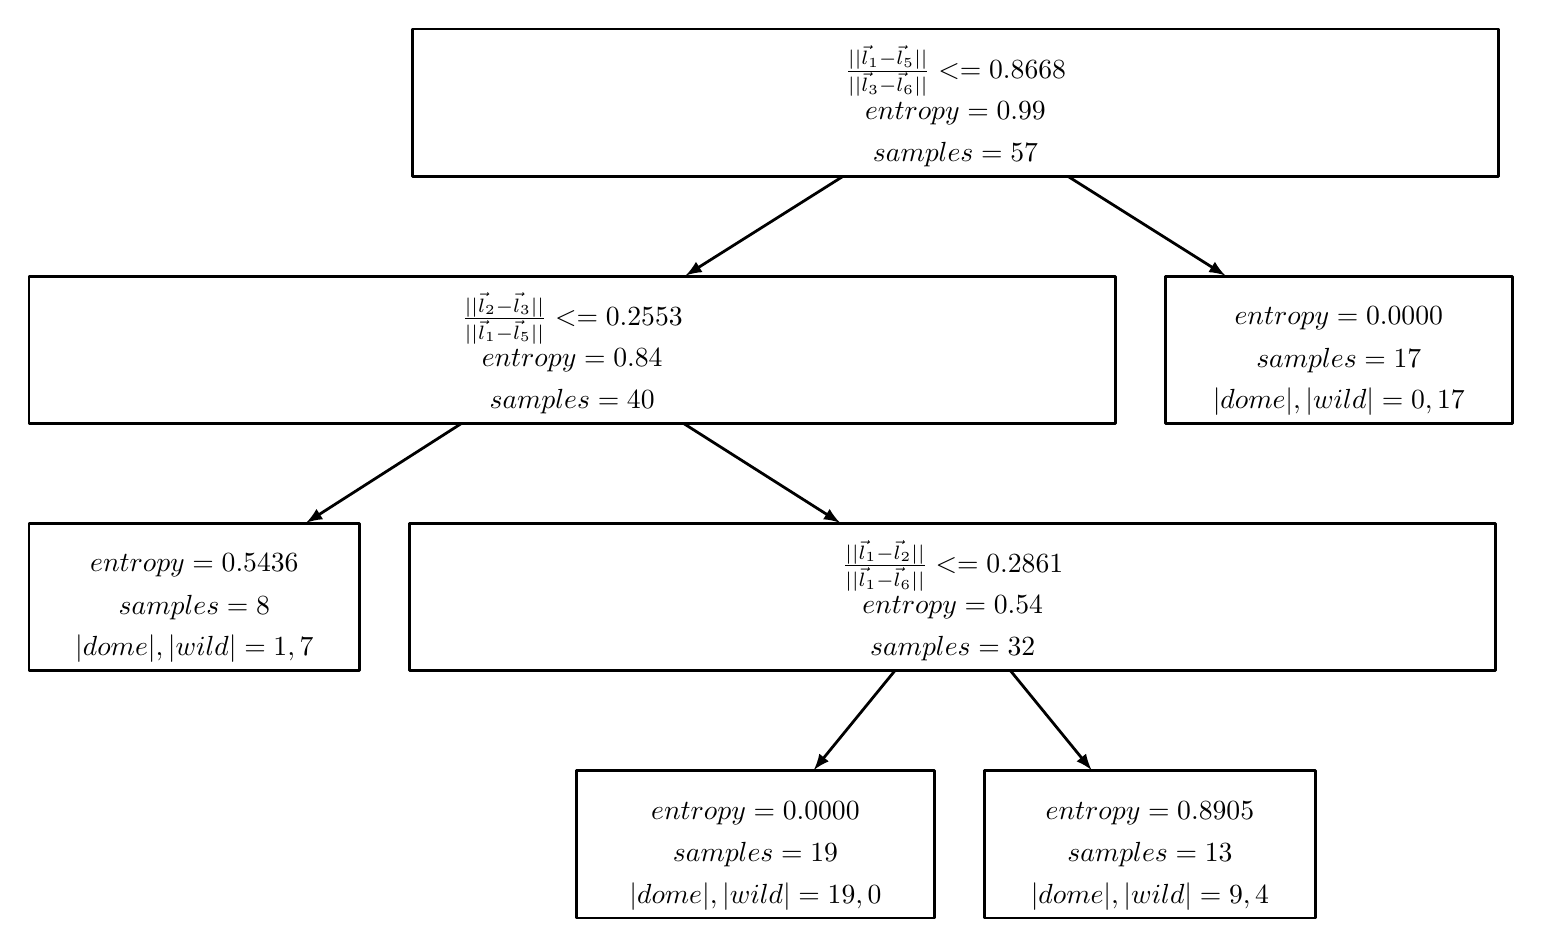
\begin{tikzpicture}[>=latex,line join=bevel,]
  \pgfsetlinewidth{1bp}
%%
\pgfsetcolor{black}
  % Edge: 0 -> 6
  \draw [->] (374.16bp,266.87bp) .. controls (389.18bp,257.39bp) and (406.38bp,246.55bp)  .. (430.66bp,231.25bp);
  % Edge: 3 -> 5
  \draw [->] (353.42bp,88.868bp) .. controls (360.51bp,80.184bp) and (368.53bp,70.35bp)  .. (382.49bp,53.25bp);
  % Edge: 1 -> 2
  \draw [->] (155.43bp,177.87bp) .. controls (140.62bp,168.39bp) and (123.67bp,157.55bp)  .. (99.752bp,142.25bp);
  % Edge: 3 -> 4
  \draw [->] (311.58bp,88.868bp) .. controls (304.49bp,80.184bp) and (296.47bp,70.35bp)  .. (282.51bp,53.25bp);
  % Edge: 0 -> 1
  \draw [->] (292.84bp,266.87bp) .. controls (277.82bp,257.39bp) and (260.62bp,246.55bp)  .. (236.34bp,231.25bp);
  % Edge: 1 -> 3
  \draw [->] (235.86bp,177.87bp) .. controls (250.78bp,168.39bp) and (267.85bp,157.55bp)  .. (291.95bp,142.25bp);
  % Node: 1
\begin{scope}
  \definecolor{strokecol}{rgb}{0.0,0.0,0.0};
  \pgfsetstrokecolor{strokecol}
  \draw (391.0bp,231.0bp) -- (0.0bp,231.0bp) -- (0.0bp,178.0bp) -- (391.0bp,178.0bp) -- cycle;
  \draw (195.5bp,215.8bp) node {$\frac{||\vec{l}_2 - \vec{l}_3||}{||\vec{l}_1 - \vec{l}_5||} <= 0.2553$};
  \draw (195.5bp,200.8bp) node {$entropy = 0.84$};
  \draw (195.5bp,185.8bp) node {$samples = 40$};
\end{scope}
  % Node: 0
\begin{scope}
  \definecolor{strokecol}{rgb}{0.0,0.0,0.0};
  \pgfsetstrokecolor{strokecol}
  \draw (529.0bp,320.0bp) -- (138.0bp,320.0bp) -- (138.0bp,267.0bp) -- (529.0bp,267.0bp) -- cycle;
  \draw (333.5bp,304.8bp) node {$\frac{||\vec{l}_1 - \vec{l}_5||}{||\vec{l}_3 - \vec{l}_6||} <= 0.8668$};
  \draw (333.5bp,289.8bp) node {$entropy = 0.99$};
  \draw (333.5bp,274.8bp) node {$samples = 57$};
\end{scope}
  % Node: 3
\begin{scope}
  \definecolor{strokecol}{rgb}{0.0,0.0,0.0};
  \pgfsetstrokecolor{strokecol}
  \draw (528.0bp,142.0bp) -- (137.0bp,142.0bp) -- (137.0bp,89.0bp) -- (528.0bp,89.0bp) -- cycle;
  \draw (332.5bp,126.8bp) node {$\frac{||\vec{l}_1 - \vec{l}_2||}{||\vec{l}_1 - \vec{l}_6||} <= 0.2861$};
  \draw (332.5bp,111.8bp) node {$entropy = 0.54$};
  \draw (332.5bp,96.8bp) node {$samples = 32$};
\end{scope}
  % Node: 2
\begin{scope}
  \definecolor{strokecol}{rgb}{0.0,0.0,0.0};
  \pgfsetstrokecolor{strokecol}
  \draw (119.0bp,142.0bp) -- (0.0bp,142.0bp) -- (0.0bp,89.0bp) -- (119.0bp,89.0bp) -- cycle;
  \draw (59.5bp,126.8bp) node {$entropy = 0.5436$};
  \draw (59.5bp,111.8bp) node {$samples = 8$};
  \draw (59.5bp,96.8bp) node {$|dome|, |wild| = 1,  7$};
\end{scope}
  % Node: 5
\begin{scope}
  \definecolor{strokecol}{rgb}{0.0,0.0,0.0};
  \pgfsetstrokecolor{strokecol}
  \draw (463.0bp,53.0bp) -- (344.0bp,53.0bp) -- (344.0bp,0.0bp) -- (463.0bp,0.0bp) -- cycle;
  \draw (403.5bp,37.8bp) node {$entropy = 0.8905$};
  \draw (403.5bp,22.8bp) node {$samples = 13$};
  \draw (403.5bp,7.8bp) node {$|dome|, |wild| = 9,  4$};
\end{scope}
  % Node: 4
\begin{scope}
  \definecolor{strokecol}{rgb}{0.0,0.0,0.0};
  \pgfsetstrokecolor{strokecol}
  \draw (326.0bp,53.0bp) -- (197.0bp,53.0bp) -- (197.0bp,0.0bp) -- (326.0bp,0.0bp) -- cycle;
  \draw (261.5bp,37.8bp) node {$entropy = 0.0000$};
  \draw (261.5bp,22.8bp) node {$samples = 19$};
  \draw (261.5bp,7.8bp) node {$|dome|, |wild| = 19,   0$};
\end{scope}
  % Node: 6
\begin{scope}
  \definecolor{strokecol}{rgb}{0.0,0.0,0.0};
  \pgfsetstrokecolor{strokecol}
  \draw (534.0bp,231.0bp) -- (409.0bp,231.0bp) -- (409.0bp,178.0bp) -- (534.0bp,178.0bp) -- cycle;
  \draw (471.5bp,215.8bp) node {$entropy = 0.0000$};
  \draw (471.5bp,200.8bp) node {$samples = 17$};
  \draw (471.5bp,185.8bp) node {$|dome|, |wild| = 0,  17$};
\end{scope}
%
\end{tikzpicture}
}

	\end{subfigure}
	\caption{Decision tree for measurable values}
	\label{fig:result-decision-tree}
\end{figure}

As the split criterion information gain proved to yield better results than using the Gini index. As for the landmark extraction method, space partitioning was increasing the result quality as well. Since they are more easy to locate as well, this proved to be a perk. As for the depth and the minimum number of samples per leaf, we decided to favor a decision tree depth of $3$ with minimum $6$ samples per leaf over a depth of $2$. While a depth of $2$ would require the researcher to take fewer measurements, only one of the branches of the tree actually has this depth, which leaves the researcher with often taking fewer measurements.

With this configuration, the decision tree shown in Figure \ref{fig:result-decision-tree} is trained. The cross-validation accuracy lies at about $77\%$ which is a sufficiently high value for a training set of this size. A researcher in the field would need to take two to six measurements on the bone to determine the type of bone.

\chapter{Conclusion}
\label{chapter:conclusion}

\section{Summary}

In this thesis we have presented a novel method to analyze shapes for local variances between classes. First the bone outlines were segmented from an image of the bone in a semi-automatic fashion. Based on a support vector machine we calculated separability metrics for windows we cut from these outlines. We introduced several features that can be used to train the SVM and compared them. We have validated the algorithm using synthetic data that was generated using randomized class instances. In the end this method was applied to bone findings of domestic and wild sheep to find locations where these types differ significantly.

Additionally we presented a decision tree with which domestic and wild sheep can be classified in the field using only a ruler or caliper rule. This method is based on landmarks that need to be located on the bone by the researcher.

\section{Discussion}

The method we presented has some advantages over geometric morphometrics or comparing the mean outlines of the bone. In common geometric morphometric approaches, the only way to locate the differences on the bone is to look at the thin plate spline transformation, which only shows the landmarks. Our method provides another way that concisely shows the location of significant differences on the bone. Additionally, compared to geometrical morphometrics, the process is a lot more automated, without the need to set landmarks or manually tracing the outline between landmarks.

While we can show these differences, we cannot characterize them other than interpreting the raw data or the mean outlines. Because of that, the reason why the bone is separable at a certain location stays hidden in the algorithm. This is not the case in geometric morphometrics where the principal component that correlates simply can be analyzed. With some research this might be possible as well for this algorithm.

A more significant disadvantage of this method is that, in its current implementation, it will only work on round shapes where every point on the outline is reachable by ray casting from the center of the shape. Otherwise the windows will not be extracted correctly. While this holds true for the Tali bones we examined, it severely limits the shape space we can work with.

Compared to other shape description methods in data science, we use local data to find key points on a shape, while most other approaches describe the shape as a whole. This allows us to evaluate the shape only at certain points when this method is used as a classifier.

\section{Future Work}

While we are using the algorithm as a method to find separable points, it should be easily possible to extend it to be a classifier that can classify shapes of the respective classes it was trained with. Since a trained SVM already exists at every point that separates the classes, these SVMs can be evaluated with new shapes and weighted to create a classifier which works on these points.

Another apparent extension is to make the algorithm work with three dimensional data. For this purpose the evaluation points would need to be selected using two angles and the window would become an area cut from the surface of the three dimensional bone model. Non-uniform Rational B-Splines could be used instead of B-Splines to describe the surface of the bone.

To cope with the limitations on shapes that can be used with the algorithm, a different method to find the evaluation points on the outline could be implemented. Instead of using angles, spline parameters could be used to select evaluation points. It would be required to synchronize these parameters somehow to extract semantically similar windows, which could be achieved by using dynamic time warping.

Additionally since we implemented relatively simple features in this thesis, other more sophisticated features could be used to train and evaluate the SVM.

\appendix

\chapter{Mathematical Basics}

\begin{table}[h]
	\begin{center}
		\begin{tabular}{|r|r|r|}
			\hline
			\makebox[1cm]{$f_1$} & \makebox[1cm]{$f_2$} & \makebox[1cm]{$c$} \\
			\hline
			\hline 1 & 2 & 0 \\
			\hline 2 & 1 & 0 \\
			\hline 2 & 2 & 0 \\
			\hline 0 & 2 & 1 \\
			\hline 0 & 0 & 1 \\
			\hline 2 & 0 & 1 \\
			\hline
		\end{tabular}
	\end{center}
	\caption{Training data for the example decision tree.}
	\label{appendix:table:decision-tree}
\end{table}

\chapter{Landmark Extraction}

\begin{table}[h]
    \begin{center}
        \begin{tabular}{|r|r|r|r|}
            \hline \makebox[3cm]{Landmark No} & \makebox[1cm]{$\alpha_{min}$} & \makebox[1cm]{$\alpha_{max}$} & \makebox[2cm]{Type} \\
            \hline\hline 1 &  $30^{\circ}$ & $90^{\circ}$ & maximum \\
            \hline 2 &  $80^{\circ}$ & $100^{\circ}$ & minimum \\
            \hline 3 &  $90^{\circ}$ & $150^{\circ}$ & maximum \\
            \hline 5 &  $170^{\circ}$ & $190^{\circ}$ & maximum \\
            \hline 6 &  $210^{\circ}$ & $270^{\circ}$ & maximum \\
            \hline 7 &  $260^{\circ}$ & $280^{\circ}$ & minimum \\
            \hline 8 &  $270^{\circ}$ & $330^{\circ}$ & maximum \\
            \hline
        \end{tabular}
    \end{center}
    \caption{Landmark Definitions for the Extraction by Angle.}
    \label{appendix:table:landmarks-angle}
\end{table}

\begin{table}[h]
    \begin{center}
        \begin{tabular}{|r|r|r|r|r|r|r|}
            \hline
            \makebox[3cm]{Landmark No} & \makebox[1cm]{$x_{min}$} & \makebox[1cm]{$x_{max}$} & \makebox[1cm]{$y_{min}$} & \makebox[1cm]{$y_{max}$} & \makebox[2cm]{Axis} & \makebox[2cm]{Type} \\
            \hline
            \hline 1 &  $0.25$ & $1$ & $0.75$ & $1.5$ & y & maximum \\
            \hline 2 &  $-0.5$ & $0.5$ & $0.75$ & $1.5$ & y & minimum \\
            \hline 3 &  $-1$ & $-0.25$ & $0.75$ & $1.5$ & y & maximum \\
            \hline 5 &  $-1$ & $-0.25$ & $-0.3$ & $0.3$ & x & minimum \\
            \hline 6 &  $-1$ & $0.25$ & $-1.5$ & $-0.75$ & y & minimum \\
            \hline 7 &  $-0.5$ & $0.5$ & $-1.5$ & $-0.75$ & y & maximum \\
            \hline 8 &  $0.25$ & $1$ & $-1.5$ & $-0.75$ & y & minimum \\
            \hline
        \end{tabular}
    \end{center}
    \caption{Landmark Definitions for the Extraction by Space Partitioning.}
    \label{appendix:table:landmarks-space}
\end{table}

\chapter{Synthetic Generation}

\begin{table}[h]
	\begin{center}
		\begin{tabular}{|r|r|r|r|}
			\hline
			\makebox[1cm]{$i$} & \makebox[1cm]{$\mu_i$} & \makebox[1cm]{$h_i$} & \makebox[1cm]{$\sigma_i$} \\
			\hline
			\hline 1 & $45^\circ$ & 0.1 & 20 \\
			\hline 2 & $60^\circ$ & 0.3 & 15 \\
			\hline 3 & $90^\circ$ & -0.2 & 10 \\
			\hline 4 & $120^\circ$ & 0.3 & 15 \\
			\hline 5 & $180^\circ$ & 0.1 & 5 \\
			\hline 6 & $240^\circ$ & 0.3 & 15 \\
			\hline 7 & $270^\circ$ & -0.2 & 10 \\
			\hline 8 & $300^\circ$ & 0.3 & 15 \\
			\hline
		\end{tabular}
	\end{center}
	\caption{Definition of a synthetic bone shape.}
	\label{appendix:table:synthetic-bone}
\end{table}

\begin{table}[h]
	\begin{center}
		\begin{tabular}{|r|r|r|r|}
			\hline
			\makebox[1cm]{$i$} & \makebox[1cm]{$\mu_i$} & \makebox[1cm]{$h_i$} & \makebox[1cm]{$\sigma_i$} \\
			\hline
			\hline 5 & $180^\circ$ & 0.0 & 5 \\
			\hline
		\end{tabular}
	\end{center}
	\caption{Adaptations from Table \ref{appendix:table:synthetic-bone} for a missing feature.}
	\label{appendix:table:synthetic-bone-missing}
\end{table}

\begin{table}[h]
	\begin{center}
		\begin{tabular}{|r|r|r|r|}
			\hline
			\makebox[1cm]{$i$} & \makebox[1cm]{$\mu_i$} & \makebox[1cm]{$h_i$} & \makebox[1cm]{$\sigma_i$} \\
			\hline
			\hline 7 & $265^\circ$ & -0.2 & 10 \\
			\hline
		\end{tabular}
	\end{center}
	\caption{Adaptations from Table \ref{appendix:table:synthetic-bone} for a shifted feature.}
	\label{appendix:table:synthetic-bone-shifted}
\end{table}

\begin{table}[h]
	\begin{center}
		\begin{tabular}{|r|r|r|r|}
			\hline
			\makebox[1cm]{$i$} & \makebox[1cm]{$\mu_i$} & \makebox[1cm]{$h_i$} & \makebox[1cm]{$\sigma_i$} \\
			\hline
			\hline 1 & $45^\circ$ & 0.05 & 20 \\
			\hline 5 & $180^\circ$ & 0.0 & 5 \\
			\hline 7 & $265^\circ$ & -0.2 & 15 \\
			\hline
		\end{tabular}
	\end{center}
	\caption{Adaptations from Table \ref{appendix:table:synthetic-bone} for multiple differing features.}
	\label{appendix:table:synthetic-bone-all}
\end{table}

% Abbildungsverzeichnis (kann auch nach dem Inhaltsverzeichnis kommen)
\listoffigures

% Tabellenverzeichnis (kann auch nach dem Inhaltsverzeichnis kommen)
\listoftables

% Literaturverzeichnis
\bibliographystyle{dbstmpl}    % verwendet dbstmpl.bst
% alternative, vorinstallierte Stile sind z.B. plain oder abbrv
\bibliography{dbstmpl}         % verwendet dbstmpl.bib

\end{document}
